\documentclass[twoside]{book}

% Packages required by doxygen
\usepackage{fixltx2e}
\usepackage{calc}
\usepackage{doxygen}
\usepackage[export]{adjustbox} % also loads graphicx
\usepackage{graphicx}
\usepackage[utf8]{inputenc}
\usepackage{makeidx}
\usepackage{multicol}
\usepackage{multirow}
\PassOptionsToPackage{warn}{textcomp}
\usepackage{textcomp}
\usepackage[nointegrals]{wasysym}
\usepackage[table]{xcolor}

% Font selection
\usepackage[T1]{fontenc}
\usepackage[scaled=.90]{helvet}
\usepackage{courier}
\usepackage{amssymb}
\usepackage{sectsty}
\renewcommand{\familydefault}{\sfdefault}
\allsectionsfont{%
  \fontseries{bc}\selectfont%
  \color{darkgray}%
}
\renewcommand{\DoxyLabelFont}{%
  \fontseries{bc}\selectfont%
  \color{darkgray}%
}
\newcommand{\+}{\discretionary{\mbox{\scriptsize$\hookleftarrow$}}{}{}}

% Page & text layout
\usepackage{geometry}
\geometry{%
  a4paper,%
  top=2.5cm,%
  bottom=2.5cm,%
  left=2.5cm,%
  right=2.5cm%
}
\tolerance=750
\hfuzz=15pt
\hbadness=750
\setlength{\emergencystretch}{15pt}
\setlength{\parindent}{0cm}
\setlength{\parskip}{3ex plus 2ex minus 2ex}
\makeatletter
\renewcommand{\paragraph}{%
  \@startsection{paragraph}{4}{0ex}{-1.0ex}{1.0ex}{%
    \normalfont\normalsize\bfseries\SS@parafont%
  }%
}
\renewcommand{\subparagraph}{%
  \@startsection{subparagraph}{5}{0ex}{-1.0ex}{1.0ex}{%
    \normalfont\normalsize\bfseries\SS@subparafont%
  }%
}
\makeatother

% Headers & footers
\usepackage{fancyhdr}
\pagestyle{fancyplain}
\fancyhead[LE]{\fancyplain{}{\bfseries\thepage}}
\fancyhead[CE]{\fancyplain{}{}}
\fancyhead[RE]{\fancyplain{}{\bfseries\leftmark}}
\fancyhead[LO]{\fancyplain{}{\bfseries\rightmark}}
\fancyhead[CO]{\fancyplain{}{}}
\fancyhead[RO]{\fancyplain{}{\bfseries\thepage}}
\fancyfoot[LE]{\fancyplain{}{}}
\fancyfoot[CE]{\fancyplain{}{}}
\fancyfoot[RE]{\fancyplain{}{\bfseries\scriptsize Generated by Doxygen }}
\fancyfoot[LO]{\fancyplain{}{\bfseries\scriptsize Generated by Doxygen }}
\fancyfoot[CO]{\fancyplain{}{}}
\fancyfoot[RO]{\fancyplain{}{}}
\renewcommand{\footrulewidth}{0.4pt}
\renewcommand{\chaptermark}[1]{%
  \markboth{#1}{}%
}
\renewcommand{\sectionmark}[1]{%
  \markright{\thesection\ #1}%
}

% Indices & bibliography
\usepackage{natbib}
\usepackage[titles]{tocloft}
\setcounter{tocdepth}{3}
\setcounter{secnumdepth}{5}
\makeindex

% Hyperlinks (required, but should be loaded last)
\usepackage{ifpdf}
\ifpdf
  \usepackage[pdftex,pagebackref=true]{hyperref}
\else
  \usepackage[ps2pdf,pagebackref=true]{hyperref}
\fi
\hypersetup{%
  colorlinks=true,%
  linkcolor=blue,%
  citecolor=blue,%
  unicode%
}

% Custom commands
\newcommand{\clearemptydoublepage}{%
  \newpage{\pagestyle{empty}\cleardoublepage}%
}

\usepackage{caption}
\captionsetup{labelsep=space,justification=centering,font={bf},singlelinecheck=off,skip=4pt,position=top}

%===== C O N T E N T S =====

\begin{document}

% Titlepage & ToC
\hypersetup{pageanchor=false,
             bookmarksnumbered=true,
             pdfencoding=unicode
            }
\pagenumbering{alph}
\begin{titlepage}
\vspace*{7cm}
\begin{center}%
{\Large My Project }\\
\vspace*{1cm}
{\large Generated by Doxygen 1.8.14}\\
\end{center}
\end{titlepage}
\clearemptydoublepage
\pagenumbering{roman}
\tableofcontents
\clearemptydoublepage
\pagenumbering{arabic}
\hypersetup{pageanchor=true}

%--- Begin generated contents ---
\chapter{Hierarchical Index}
\section{Class Hierarchy}
This inheritance list is sorted roughly, but not completely, alphabetically\+:\begin{DoxyCompactList}
\item \contentsline{section}{io.\+github.\+syzygy2048.\+radcloud.\+Document\+Manager}{\pageref{classio_1_1github_1_1syzygy2048_1_1radcloud_1_1_document_manager}}{}
\item \contentsline{section}{io.\+github.\+syzygy2048.\+radcloud.\+Document\+Manager.\+Ellipse}{\pageref{classio_1_1github_1_1syzygy2048_1_1radcloud_1_1_document_manager_1_1_ellipse}}{}
\item \contentsline{section}{io.\+github.\+syzygy2048.\+radcloud.\+Spiral\+Generator}{\pageref{classio_1_1github_1_1syzygy2048_1_1radcloud_1_1_spiral_generator}}{}
\item \contentsline{section}{io.\+github.\+syzygy2048.\+radcloud.\+Document\+Manager.\+Vec2}{\pageref{classio_1_1github_1_1syzygy2048_1_1radcloud_1_1_document_manager_1_1_vec2}}{}
\item \contentsline{section}{io.\+github.\+syzygy2048.\+radcloud.\+Word}{\pageref{classio_1_1github_1_1syzygy2048_1_1radcloud_1_1_word}}{}
\item App\+Compat\+Activity\begin{DoxyCompactList}
\item \contentsline{section}{io.\+github.\+syzygy2048.\+radcloud.\+Loading\+Screen\+Activity}{\pageref{classio_1_1github_1_1syzygy2048_1_1radcloud_1_1_loading_screen_activity}}{}
\item \contentsline{section}{io.\+github.\+syzygy2048.\+radcloud.\+Main\+Activity}{\pageref{classio_1_1github_1_1syzygy2048_1_1radcloud_1_1_main_activity}}{}
\item \contentsline{section}{io.\+github.\+syzygy2048.\+radcloud.\+Rad\+Cloud\+Activity}{\pageref{classio_1_1github_1_1syzygy2048_1_1radcloud_1_1_rad_cloud_activity}}{}
\end{DoxyCompactList}
\end{DoxyCompactList}

\chapter{Class Index}
\section{Class List}
Here are the classes, structs, unions and interfaces with brief descriptions\+:\begin{DoxyCompactList}
\item\contentsline{section}{\mbox{\hyperlink{classio_1_1github_1_1syzygy2048_1_1radcloud_1_1_document_manager}{io.\+github.\+syzygy2048.\+radcloud.\+Document\+Manager}} }{\pageref{classio_1_1github_1_1syzygy2048_1_1radcloud_1_1_document_manager}}{}
\item\contentsline{section}{\mbox{\hyperlink{classio_1_1github_1_1syzygy2048_1_1radcloud_1_1_document_manager_1_1_ellipse}{io.\+github.\+syzygy2048.\+radcloud.\+Document\+Manager.\+Ellipse}} }{\pageref{classio_1_1github_1_1syzygy2048_1_1radcloud_1_1_document_manager_1_1_ellipse}}{}
\item\contentsline{section}{\mbox{\hyperlink{classio_1_1github_1_1syzygy2048_1_1radcloud_1_1_loading_screen_activity}{io.\+github.\+syzygy2048.\+radcloud.\+Loading\+Screen\+Activity}} }{\pageref{classio_1_1github_1_1syzygy2048_1_1radcloud_1_1_loading_screen_activity}}{}
\item\contentsline{section}{\mbox{\hyperlink{classio_1_1github_1_1syzygy2048_1_1radcloud_1_1_main_activity}{io.\+github.\+syzygy2048.\+radcloud.\+Main\+Activity}} }{\pageref{classio_1_1github_1_1syzygy2048_1_1radcloud_1_1_main_activity}}{}
\item\contentsline{section}{\mbox{\hyperlink{classio_1_1github_1_1syzygy2048_1_1radcloud_1_1_rad_cloud_activity}{io.\+github.\+syzygy2048.\+radcloud.\+Rad\+Cloud\+Activity}} }{\pageref{classio_1_1github_1_1syzygy2048_1_1radcloud_1_1_rad_cloud_activity}}{}
\item\contentsline{section}{\mbox{\hyperlink{classio_1_1github_1_1syzygy2048_1_1radcloud_1_1_spiral_generator}{io.\+github.\+syzygy2048.\+radcloud.\+Spiral\+Generator}} }{\pageref{classio_1_1github_1_1syzygy2048_1_1radcloud_1_1_spiral_generator}}{}
\item\contentsline{section}{\mbox{\hyperlink{classio_1_1github_1_1syzygy2048_1_1radcloud_1_1_document_manager_1_1_vec2}{io.\+github.\+syzygy2048.\+radcloud.\+Document\+Manager.\+Vec2}} }{\pageref{classio_1_1github_1_1syzygy2048_1_1radcloud_1_1_document_manager_1_1_vec2}}{}
\item\contentsline{section}{\mbox{\hyperlink{classio_1_1github_1_1syzygy2048_1_1radcloud_1_1_word}{io.\+github.\+syzygy2048.\+radcloud.\+Word}} }{\pageref{classio_1_1github_1_1syzygy2048_1_1radcloud_1_1_word}}{}
\end{DoxyCompactList}

\chapter{Class Documentation}
\hypertarget{classio_1_1github_1_1syzygy2048_1_1radcloud_1_1_document_manager}{}\section{io.\+github.\+syzygy2048.\+radcloud.\+Document\+Manager Class Reference}
\label{classio_1_1github_1_1syzygy2048_1_1radcloud_1_1_document_manager}\index{io.\+github.\+syzygy2048.\+radcloud.\+Document\+Manager@{io.\+github.\+syzygy2048.\+radcloud.\+Document\+Manager}}
\subsection*{Classes}
\begin{DoxyCompactItemize}
\item 
class \mbox{\hyperlink{classio_1_1github_1_1syzygy2048_1_1radcloud_1_1_document_manager_1_1_ellipse}{Ellipse}}
\item 
class \mbox{\hyperlink{classio_1_1github_1_1syzygy2048_1_1radcloud_1_1_document_manager_1_1_vec2}{Vec2}}
\end{DoxyCompactItemize}
\subsection*{Public Member Functions}
\begin{DoxyCompactItemize}
\item 
void \mbox{\hyperlink{classio_1_1github_1_1syzygy2048_1_1radcloud_1_1_document_manager_a00bcd6e86e3cd7b82122d06c09135963}{process}} ()
\item 
void \mbox{\hyperlink{classio_1_1github_1_1syzygy2048_1_1radcloud_1_1_document_manager_ae2fd7551555ca6e97cab1ea87a4ab477}{read\+Document}} (Context ctx, int resource\+Id, String document\+Name)
\item 
void \mbox{\hyperlink{classio_1_1github_1_1syzygy2048_1_1radcloud_1_1_document_manager_a917f02cb6436d96077b0e093751710ec}{read\+Document}} (String path, String document\+Name)  throws File\+Not\+Found\+Exception 
\item 
Hash\+Map$<$ String, Integer $>$ \mbox{\hyperlink{classio_1_1github_1_1syzygy2048_1_1radcloud_1_1_document_manager_a64e9767900c245d1c77cdf12dc92c807}{get\+Document\+List}} ()
\item 
Array\+List$<$ \mbox{\hyperlink{classio_1_1github_1_1syzygy2048_1_1radcloud_1_1_word}{Word}} $>$ \mbox{\hyperlink{classio_1_1github_1_1syzygy2048_1_1radcloud_1_1_document_manager_a8868166a68ecfa01206268e13c3560ea}{get\+Word\+List}} ()
\item 
void \mbox{\hyperlink{classio_1_1github_1_1syzygy2048_1_1radcloud_1_1_document_manager_ac4e94090407ff6f6c1d3b2f7c02cec83}{resolve\+Overlaps}} ()
\end{DoxyCompactItemize}
\subsection*{Static Public Member Functions}
\begin{DoxyCompactItemize}
\item 
static \mbox{\hyperlink{classio_1_1github_1_1syzygy2048_1_1radcloud_1_1_document_manager}{Document\+Manager}} \mbox{\hyperlink{classio_1_1github_1_1syzygy2048_1_1radcloud_1_1_document_manager_abb1a711c0690a259a1081c573396b84a}{get\+Instance}} ()
\end{DoxyCompactItemize}
\subsection*{Private Member Functions}
\begin{DoxyCompactItemize}
\item 
void \mbox{\hyperlink{classio_1_1github_1_1syzygy2048_1_1radcloud_1_1_document_manager_aecdf1d11ec1b9a2db9cdb0f60b1c1184}{add}} (String document, String term)
\item 
void \mbox{\hyperlink{classio_1_1github_1_1syzygy2048_1_1radcloud_1_1_document_manager_adcf3b63232181ceb86abc91a5a37cf0f}{calculate\+Term\+Frequency}} ()
\item 
void \mbox{\hyperlink{classio_1_1github_1_1syzygy2048_1_1radcloud_1_1_document_manager_aa220917ccab9869414a201361ba1e1a9}{calculate\+Inverse\+Document\+Frequency}} ()
\item 
void \mbox{\hyperlink{classio_1_1github_1_1syzygy2048_1_1radcloud_1_1_document_manager_a9b7a1e94d648221841ecc5d5c5650f0b}{select\+Top\+Words\+Per\+Document}} ()
\item 
void \mbox{\hyperlink{classio_1_1github_1_1syzygy2048_1_1radcloud_1_1_document_manager_a7418a74e1d0a3a7677875d525a12b2f1}{calculate\+Bounding\+Boxes}} ()
\item 
void \mbox{\hyperlink{classio_1_1github_1_1syzygy2048_1_1radcloud_1_1_document_manager_a7c3bd4342ae38a0876b0fecdddf95de7}{calculate\+Document\+Vectors}} ()
\item 
void \mbox{\hyperlink{classio_1_1github_1_1syzygy2048_1_1radcloud_1_1_document_manager_a9fab6a75480c9f0aa1fa2085359dd8fa}{process\+Input\+File}} (Input\+Stream input\+Stream, String document\+Name)
\item 
void \mbox{\hyperlink{classio_1_1github_1_1syzygy2048_1_1radcloud_1_1_document_manager_a42be8000ada29b9f9a45a48f0804f760}{calculate\+Position}} ()
\item 
void \mbox{\hyperlink{classio_1_1github_1_1syzygy2048_1_1radcloud_1_1_document_manager_a0cc957e8369ea7136b5b7eacc4ce8a13}{fix\+Overlaps}} (\mbox{\hyperlink{classio_1_1github_1_1syzygy2048_1_1radcloud_1_1_word}{Word}} word, int i)
\item 
boolean \mbox{\hyperlink{classio_1_1github_1_1syzygy2048_1_1radcloud_1_1_document_manager_a46efa97bb7935e67250b7386c2c31da7}{check\+For\+Overlap}} (List$<$ \mbox{\hyperlink{classio_1_1github_1_1syzygy2048_1_1radcloud_1_1_word}{Word}} $>$ placed\+Words, \mbox{\hyperlink{classio_1_1github_1_1syzygy2048_1_1radcloud_1_1_word}{Word}} word)
\item 
boolean \mbox{\hyperlink{classio_1_1github_1_1syzygy2048_1_1radcloud_1_1_document_manager_a418e7db1e3a441cbcf4b5bd2b90b31fd}{outside\+The\+Ring}} (\mbox{\hyperlink{classio_1_1github_1_1syzygy2048_1_1radcloud_1_1_word}{Word}} word)
\item 
boolean \mbox{\hyperlink{classio_1_1github_1_1syzygy2048_1_1radcloud_1_1_document_manager_acf53af046d9fbe0df0dd1c062a2c2398}{overlaps}} (Rect bb1, Rect bb2)
\end{DoxyCompactItemize}
\subsection*{Private Attributes}
\begin{DoxyCompactItemize}
\item 
Hash\+Map$<$ String, Integer $>$ \mbox{\hyperlink{classio_1_1github_1_1syzygy2048_1_1radcloud_1_1_document_manager_aebb5c1d79109552b3b85ce9ee7a971ab}{document\+List}} = new Hash\+Map$<$$>$()
\item 
Hash\+Map$<$ String, \mbox{\hyperlink{classio_1_1github_1_1syzygy2048_1_1radcloud_1_1_document_manager_1_1_vec2}{Vec2}} $>$ \mbox{\hyperlink{classio_1_1github_1_1syzygy2048_1_1radcloud_1_1_document_manager_ae09195d3ddec27f4cf496d0ed87bab26}{document\+Vectors}} = new Hash\+Map$<$$>$()
\item 
Array\+List$<$ \mbox{\hyperlink{classio_1_1github_1_1syzygy2048_1_1radcloud_1_1_word}{Word}} $>$ \mbox{\hyperlink{classio_1_1github_1_1syzygy2048_1_1radcloud_1_1_document_manager_a723b2b3488074851d4523c37a33ce6b8}{word\+List}} = new Array\+List$<$$>$()
\item 
\mbox{\hyperlink{classio_1_1github_1_1syzygy2048_1_1radcloud_1_1_document_manager_1_1_ellipse}{Ellipse}} \mbox{\hyperlink{classio_1_1github_1_1syzygy2048_1_1radcloud_1_1_document_manager_a6122082006d279500cdcc27e03298310}{frame}} = new \mbox{\hyperlink{classio_1_1github_1_1syzygy2048_1_1radcloud_1_1_document_manager_1_1_ellipse}{Ellipse}}()
\item 
String \mbox{[}$\,$\mbox{]} \mbox{\hyperlink{classio_1_1github_1_1syzygy2048_1_1radcloud_1_1_document_manager_ad6df7df2e34771a53fd15b80e8fc24e0}{stopwords}} = new String\mbox{[}$\,$\mbox{]}\{\char`\"{}\textquotesingle{}ll\char`\"{}, \char`\"{}\textquotesingle{}tis\char`\"{}, \char`\"{}\textquotesingle{}twas\char`\"{}, \char`\"{}\textquotesingle{}ve\char`\"{}, \char`\"{}10\char`\"{}, \char`\"{}39\char`\"{}, \char`\"{}a\char`\"{}, \char`\"{}a\textquotesingle{}s\char`\"{}, \char`\"{}able\char`\"{}, \char`\"{}ableabout\char`\"{}, \char`\"{}about\char`\"{}, \char`\"{}above\char`\"{}, \char`\"{}abroad\char`\"{}, \char`\"{}abst\char`\"{}, \char`\"{}accordance\char`\"{}, \char`\"{}according\char`\"{}, \char`\"{}accordingly\char`\"{}, \char`\"{}across\char`\"{}, \char`\"{}act\char`\"{}, \char`\"{}actually\char`\"{}, \char`\"{}ad\char`\"{}, \char`\"{}added\char`\"{}, \char`\"{}adj\char`\"{}, \char`\"{}adopted\char`\"{}, \char`\"{}ae\char`\"{}, \char`\"{}af\char`\"{}, \char`\"{}affected\char`\"{}, \char`\"{}affecting\char`\"{}, \char`\"{}affects\char`\"{}, \char`\"{}after\char`\"{}, \char`\"{}afterwards\char`\"{}, \char`\"{}ag\char`\"{}, \char`\"{}again\char`\"{}, \char`\"{}against\char`\"{}, \char`\"{}ago\char`\"{}, \char`\"{}ah\char`\"{}, \char`\"{}ahead\char`\"{}, \char`\"{}ai\char`\"{}, \char`\"{}ain\textquotesingle{}t\char`\"{}, \char`\"{}aint\char`\"{}, \char`\"{}al\char`\"{}, \char`\"{}all\char`\"{}, \char`\"{}allow\char`\"{}, \char`\"{}allows\char`\"{}, \char`\"{}almost\char`\"{}, \char`\"{}alone\char`\"{}, \char`\"{}along\char`\"{}, \char`\"{}alongside\char`\"{}, \char`\"{}already\char`\"{}, \char`\"{}also\char`\"{}, \char`\"{}although\char`\"{}, \char`\"{}always\char`\"{}, \char`\"{}am\char`\"{}, \char`\"{}amid\char`\"{}, \char`\"{}amidst\char`\"{}, \char`\"{}among\char`\"{}, \char`\"{}amongst\char`\"{}, \char`\"{}amoungst\char`\"{}, \char`\"{}amount\char`\"{}, \char`\"{}an\char`\"{}, \char`\"{}and\char`\"{}, \char`\"{}announce\char`\"{}, \char`\"{}another\char`\"{}, \char`\"{}any\char`\"{}, \char`\"{}anybody\char`\"{}, \char`\"{}anyhow\char`\"{}, \char`\"{}anymore\char`\"{}, \char`\"{}anyone\char`\"{}, \char`\"{}anything\char`\"{}, \char`\"{}anyway\char`\"{}, \char`\"{}anyways\char`\"{}, \char`\"{}anywhere\char`\"{}, \char`\"{}ao\char`\"{}, \char`\"{}apart\char`\"{}, \char`\"{}apparently\char`\"{}, \char`\"{}appear\char`\"{}, \char`\"{}appreciate\char`\"{}, \char`\"{}appropriate\char`\"{}, \char`\"{}approximately\char`\"{}, \char`\"{}aq\char`\"{}, \char`\"{}ar\char`\"{}, \char`\"{}are\char`\"{}, \char`\"{}area\char`\"{}, \char`\"{}areas\char`\"{}, \char`\"{}aren\char`\"{}, \char`\"{}aren\textquotesingle{}t\char`\"{}, \char`\"{}arent\char`\"{}, \char`\"{}arise\char`\"{}, \char`\"{}around\char`\"{}, \char`\"{}arpa\char`\"{}, \char`\"{}as\char`\"{}, \char`\"{}aside\char`\"{}, \char`\"{}ask\char`\"{}, \char`\"{}asked\char`\"{}, \char`\"{}asking\char`\"{}, \char`\"{}asks\char`\"{}, \char`\"{}associated\char`\"{}, \char`\"{}at\char`\"{}, \char`\"{}au\char`\"{}, \char`\"{}auth\char`\"{}, \char`\"{}available\char`\"{}, \char`\"{}aw\char`\"{}, \char`\"{}away\char`\"{}, \char`\"{}awfully\char`\"{}, \char`\"{}az\char`\"{}, \char`\"{}b\char`\"{}, \char`\"{}ba\char`\"{}, \char`\"{}back\char`\"{}, \char`\"{}backed\char`\"{}, \char`\"{}backing\char`\"{}, \char`\"{}backs\char`\"{}, \char`\"{}backward\char`\"{}, \char`\"{}backwards\char`\"{}, \char`\"{}bb\char`\"{}, \char`\"{}bd\char`\"{}, \char`\"{}be\char`\"{}, \char`\"{}became\char`\"{}, \char`\"{}because\char`\"{}, \char`\"{}become\char`\"{}, \char`\"{}becomes\char`\"{}, \char`\"{}becoming\char`\"{}, \char`\"{}been\char`\"{}, \char`\"{}before\char`\"{}, \char`\"{}beforehand\char`\"{}, \char`\"{}began\char`\"{}, \char`\"{}begin\char`\"{}, \char`\"{}beginning\char`\"{}, \char`\"{}beginnings\char`\"{}, \char`\"{}begins\char`\"{}, \char`\"{}behind\char`\"{}, \char`\"{}being\char`\"{}, \char`\"{}beings\char`\"{}, \char`\"{}believe\char`\"{}, \char`\"{}below\char`\"{}, \char`\"{}beside\char`\"{}, \char`\"{}besides\char`\"{}, \char`\"{}best\char`\"{}, \char`\"{}better\char`\"{}, \char`\"{}between\char`\"{}, \char`\"{}beyond\char`\"{}, \char`\"{}bf\char`\"{}, \char`\"{}bg\char`\"{}, \char`\"{}bh\char`\"{}, \char`\"{}bi\char`\"{}, \char`\"{}big\char`\"{}, \char`\"{}bill\char`\"{}, \char`\"{}billion\char`\"{}, \char`\"{}biol\char`\"{}, \char`\"{}bj\char`\"{}, \char`\"{}bm\char`\"{}, \char`\"{}bn\char`\"{}, \char`\"{}bo\char`\"{}, \char`\"{}both\char`\"{}, \char`\"{}bottom\char`\"{}, \char`\"{}br\char`\"{}, \char`\"{}brief\char`\"{}, \char`\"{}briefly\char`\"{}, \char`\"{}bs\char`\"{}, \char`\"{}bt\char`\"{}, \char`\"{}but\char`\"{}, \char`\"{}buy\char`\"{}, \char`\"{}bv\char`\"{}, \char`\"{}bw\char`\"{}, \char`\"{}by\char`\"{}, \char`\"{}bz\char`\"{}, \char`\"{}c\char`\"{}, \char`\"{}c\textquotesingle{}mon\char`\"{}, \char`\"{}c\textquotesingle{}s\char`\"{}, \char`\"{}ca\char`\"{}, \char`\"{}call\char`\"{}, \char`\"{}came\char`\"{}, \char`\"{}can\char`\"{}, \char`\"{}can\textquotesingle{}t\char`\"{}, \char`\"{}cannot\char`\"{}, \char`\"{}cant\char`\"{}, \char`\"{}caption\char`\"{}, \char`\"{}case\char`\"{}, \char`\"{}cases\char`\"{}, \char`\"{}cause\char`\"{}, \char`\"{}causes\char`\"{}, \char`\"{}cc\char`\"{}, \char`\"{}cd\char`\"{}, \char`\"{}certain\char`\"{}, \char`\"{}certainly\char`\"{}, \char`\"{}cf\char`\"{}, \char`\"{}cg\char`\"{}, \char`\"{}ch\char`\"{}, \char`\"{}changes\char`\"{}, \char`\"{}ci\char`\"{}, \char`\"{}ck\char`\"{}, \char`\"{}cl\char`\"{}, \char`\"{}clear\char`\"{}, \char`\"{}clearly\char`\"{}, \char`\"{}click\char`\"{}, \char`\"{}cm\char`\"{}, \char`\"{}cmon\char`\"{}, \char`\"{}cn\char`\"{}, \char`\"{}co\char`\"{}, \char`\"{}co.\char`\"{}, \char`\"{}com\char`\"{}, \char`\"{}come\char`\"{}, \char`\"{}comes\char`\"{}, \char`\"{}computer\char`\"{}, \char`\"{}con\char`\"{}, \char`\"{}concerning\char`\"{}, \char`\"{}consequently\char`\"{}, \char`\"{}consider\char`\"{}, \char`\"{}considering\char`\"{}, \char`\"{}contain\char`\"{}, \char`\"{}containing\char`\"{}, \char`\"{}contains\char`\"{}, \char`\"{}copy\char`\"{}, \char`\"{}corresponding\char`\"{}, \char`\"{}could\char`\"{}, \char`\"{}could\textquotesingle{}ve\char`\"{}, \char`\"{}couldn\char`\"{}, \char`\"{}couldn\textquotesingle{}t\char`\"{}, \char`\"{}couldnt\char`\"{}, \char`\"{}course\char`\"{}, \char`\"{}cr\char`\"{}, \char`\"{}cry\char`\"{}, \char`\"{}cs\char`\"{}, \char`\"{}cu\char`\"{}, \char`\"{}currently\char`\"{}, \char`\"{}cv\char`\"{}, \char`\"{}cx\char`\"{}, \char`\"{}cy\char`\"{}, \char`\"{}cz\char`\"{}, \char`\"{}d\char`\"{}, \char`\"{}dare\char`\"{}, \char`\"{}daren\textquotesingle{}t\char`\"{}, \char`\"{}darent\char`\"{}, \char`\"{}date\char`\"{}, \char`\"{}de\char`\"{}, \char`\"{}dear\char`\"{}, \char`\"{}definitely\char`\"{}, \char`\"{}describe\char`\"{}, \char`\"{}described\char`\"{}, \char`\"{}despite\char`\"{}, \char`\"{}detail\char`\"{}, \char`\"{}did\char`\"{}, \char`\"{}didn\char`\"{}, \char`\"{}didn\textquotesingle{}t\char`\"{}, \char`\"{}didnt\char`\"{}, \char`\"{}differ\char`\"{}, \char`\"{}different\char`\"{}, \char`\"{}differently\char`\"{}, \char`\"{}directly\char`\"{}, \char`\"{}dj\char`\"{}, \char`\"{}dk\char`\"{}, \char`\"{}dm\char`\"{}, \char`\"{}do\char`\"{}, \char`\"{}does\char`\"{}, \char`\"{}doesn\char`\"{}, \char`\"{}doesn\textquotesingle{}t\char`\"{}, \char`\"{}doesnt\char`\"{}, \char`\"{}doing\char`\"{}, \char`\"{}don\char`\"{}, \char`\"{}don\textquotesingle{}t\char`\"{}, \char`\"{}done\char`\"{}, \char`\"{}dont\char`\"{}, \char`\"{}doubtful\char`\"{}, \char`\"{}down\char`\"{}, \char`\"{}downed\char`\"{}, \char`\"{}downing\char`\"{}, \char`\"{}downs\char`\"{}, \char`\"{}downwards\char`\"{}, \char`\"{}due\char`\"{}, \char`\"{}during\char`\"{}, \char`\"{}dz\char`\"{}, \char`\"{}e\char`\"{}, \char`\"{}each\char`\"{}, \char`\"{}early\char`\"{}, \char`\"{}ec\char`\"{}, \char`\"{}ed\char`\"{}, \char`\"{}edu\char`\"{}, \char`\"{}ee\char`\"{}, \char`\"{}effect\char`\"{}, \char`\"{}eg\char`\"{}, \char`\"{}eh\char`\"{}, \char`\"{}eight\char`\"{}, \char`\"{}eighty\char`\"{}, \char`\"{}either\char`\"{}, \char`\"{}eleven\char`\"{}, \char`\"{}else\char`\"{}, \char`\"{}elsewhere\char`\"{}, \char`\"{}empty\char`\"{}, \char`\"{}end\char`\"{}, \char`\"{}ended\char`\"{}, \char`\"{}ending\char`\"{}, \char`\"{}ends\char`\"{}, \char`\"{}enough\char`\"{}, \char`\"{}entirely\char`\"{}, \char`\"{}er\char`\"{}, \char`\"{}es\char`\"{}, \char`\"{}especially\char`\"{}, \char`\"{}et\char`\"{}, \char`\"{}et-\/al\char`\"{}, \char`\"{}etc\char`\"{}, \char`\"{}even\char`\"{}, \char`\"{}evenly\char`\"{}, \char`\"{}ever\char`\"{}, \char`\"{}evermore\char`\"{}, \char`\"{}every\char`\"{}, \char`\"{}everybody\char`\"{}, \char`\"{}everyone\char`\"{}, \char`\"{}everything\char`\"{}, \char`\"{}everywhere\char`\"{}, \char`\"{}ex\char`\"{}, \char`\"{}exactly\char`\"{}, \char`\"{}example\char`\"{}, \char`\"{}except\char`\"{}, \char`\"{}f\char`\"{}, \char`\"{}face\char`\"{}, \char`\"{}faces\char`\"{}, \char`\"{}fact\char`\"{}, \char`\"{}facts\char`\"{}, \char`\"{}fairly\char`\"{}, \char`\"{}far\char`\"{}, \char`\"{}farther\char`\"{}, \char`\"{}felt\char`\"{}, \char`\"{}few\char`\"{}, \char`\"{}fewer\char`\"{}, \char`\"{}ff\char`\"{}, \char`\"{}fi\char`\"{}, \char`\"{}fifteen\char`\"{}, \char`\"{}fifth\char`\"{}, \char`\"{}fifty\char`\"{}, \char`\"{}fify\char`\"{}, \char`\"{}fill\char`\"{}, \char`\"{}find\char`\"{}, \char`\"{}finds\char`\"{}, \char`\"{}fire\char`\"{}, \char`\"{}first\char`\"{}, \char`\"{}five\char`\"{}, \char`\"{}fix\char`\"{}, \char`\"{}fj\char`\"{}, \char`\"{}fk\char`\"{}, \char`\"{}fm\char`\"{}, \char`\"{}fo\char`\"{}, \char`\"{}followed\char`\"{}, \char`\"{}following\char`\"{}, \char`\"{}follows\char`\"{}, \char`\"{}for\char`\"{}, \char`\"{}forever\char`\"{}, \char`\"{}former\char`\"{}, \char`\"{}formerly\char`\"{}, \char`\"{}forth\char`\"{}, \char`\"{}forty\char`\"{}, \char`\"{}forward\char`\"{}, \char`\"{}found\char`\"{}, \char`\"{}four\char`\"{}, \char`\"{}fr\char`\"{}, \char`\"{}free\char`\"{}, \char`\"{}from\char`\"{}, \char`\"{}front\char`\"{}, \char`\"{}full\char`\"{}, \char`\"{}fully\char`\"{}, \char`\"{}further\char`\"{}, \char`\"{}furthered\char`\"{}, \char`\"{}furthering\char`\"{}, \char`\"{}furthermore\char`\"{}, \char`\"{}furthers\char`\"{}, \char`\"{}fx\char`\"{}, \char`\"{}g\char`\"{}, \char`\"{}ga\char`\"{}, \char`\"{}gave\char`\"{}, \char`\"{}gb\char`\"{}, \char`\"{}gd\char`\"{}, \char`\"{}ge\char`\"{}, \char`\"{}general\char`\"{}, \char`\"{}generally\char`\"{}, \char`\"{}get\char`\"{}, \char`\"{}gets\char`\"{}, \char`\"{}getting\char`\"{}, \char`\"{}gf\char`\"{}, \char`\"{}gg\char`\"{}, \char`\"{}gh\char`\"{}, \char`\"{}gi\char`\"{}, \char`\"{}give\char`\"{}, \char`\"{}given\char`\"{}, \char`\"{}gives\char`\"{}, \char`\"{}giving\char`\"{}, \char`\"{}gl\char`\"{}, \char`\"{}gm\char`\"{}, \char`\"{}gmt\char`\"{}, \char`\"{}gn\char`\"{}, \char`\"{}go\char`\"{}, \char`\"{}goes\char`\"{}, \char`\"{}going\char`\"{}, \char`\"{}gone\char`\"{}, \char`\"{}good\char`\"{}, \char`\"{}goods\char`\"{}, \char`\"{}got\char`\"{}, \char`\"{}gotten\char`\"{}, \char`\"{}gov\char`\"{}, \char`\"{}gp\char`\"{}, \char`\"{}gq\char`\"{}, \char`\"{}gr\char`\"{}, \char`\"{}great\char`\"{}, \char`\"{}greater\char`\"{}, \char`\"{}greatest\char`\"{}, \char`\"{}greetings\char`\"{}, \char`\"{}group\char`\"{}, \char`\"{}grouped\char`\"{}, \char`\"{}grouping\char`\"{}, \char`\"{}groups\char`\"{}, \char`\"{}gs\char`\"{}, \char`\"{}gt\char`\"{}, \char`\"{}gu\char`\"{}, \char`\"{}gw\char`\"{}, \char`\"{}gy\char`\"{}, \char`\"{}h\char`\"{}, \char`\"{}had\char`\"{}, \char`\"{}hadn\textquotesingle{}t\char`\"{}, \char`\"{}hadnt\char`\"{}, \char`\"{}half\char`\"{}, \char`\"{}happens\char`\"{}, \char`\"{}hardly\char`\"{}, \char`\"{}has\char`\"{}, \char`\"{}hasn\char`\"{}, \char`\"{}hasn\textquotesingle{}t\char`\"{}, \char`\"{}hasnt\char`\"{}, \char`\"{}have\char`\"{}, \char`\"{}haven\char`\"{}, \char`\"{}haven\textquotesingle{}t\char`\"{}, \char`\"{}havent\char`\"{}, \char`\"{}having\char`\"{}, \char`\"{}he\char`\"{}, \char`\"{}he\textquotesingle{}d\char`\"{}, \char`\"{}he\textquotesingle{}ll\char`\"{}, \char`\"{}he\textquotesingle{}s\char`\"{}, \char`\"{}hed\char`\"{}, \char`\"{}hell\char`\"{}, \char`\"{}hello\char`\"{}, \char`\"{}help\char`\"{}, \char`\"{}hence\char`\"{}, \char`\"{}her\char`\"{}, \char`\"{}here\char`\"{}, \char`\"{}here\textquotesingle{}s\char`\"{}, \char`\"{}hereafter\char`\"{}, \char`\"{}hereby\char`\"{}, \char`\"{}herein\char`\"{}, \char`\"{}heres\char`\"{}, \char`\"{}hereupon\char`\"{}, \char`\"{}hers\char`\"{}, \char`\"{}herself\char`\"{}, \char`\"{}herse”\char`\"{}, \char`\"{}hes\char`\"{}, \char`\"{}hi\char`\"{}, \char`\"{}hid\char`\"{}, \char`\"{}high\char`\"{}, \char`\"{}higher\char`\"{}, \char`\"{}highest\char`\"{}, \char`\"{}him\char`\"{}, \char`\"{}himself\char`\"{}, \char`\"{}himse”\char`\"{}, \char`\"{}his\char`\"{}, \char`\"{}hither\char`\"{}, \char`\"{}hk\char`\"{}, \char`\"{}hm\char`\"{}, \char`\"{}hn\char`\"{}, \char`\"{}home\char`\"{}, \char`\"{}homepage\char`\"{}, \char`\"{}hopefully\char`\"{}, \char`\"{}how\char`\"{}, \char`\"{}how\textquotesingle{}d\char`\"{}, \char`\"{}how\textquotesingle{}ll\char`\"{}, \char`\"{}how\textquotesingle{}s\char`\"{}, \char`\"{}howbeit\char`\"{}, \char`\"{}however\char`\"{}, \char`\"{}hr\char`\"{}, \char`\"{}ht\char`\"{}, \char`\"{}htm\char`\"{}, \char`\"{}html\char`\"{}, \char`\"{}http\char`\"{}, \char`\"{}hu\char`\"{}, \char`\"{}hundred\char`\"{}, \char`\"{}i\char`\"{}, \char`\"{}i\textquotesingle{}d\char`\"{}, \char`\"{}i\textquotesingle{}ll\char`\"{}, \char`\"{}i\textquotesingle{}m\char`\"{}, \char`\"{}i\textquotesingle{}ve\char`\"{}, \char`\"{}i.\+e.\char`\"{}, \char`\"{}id\char`\"{}, \char`\"{}ie\char`\"{}, \char`\"{}if\char`\"{}, \char`\"{}ignored\char`\"{}, \char`\"{}ii\char`\"{}, \char`\"{}il\char`\"{}, \char`\"{}ill\char`\"{}, \char`\"{}im\char`\"{}, \char`\"{}immediate\char`\"{}, \char`\"{}immediately\char`\"{}, \char`\"{}importance\char`\"{}, \char`\"{}important\char`\"{}, \char`\"{}in\char`\"{}, \char`\"{}inasmuch\char`\"{}, \char`\"{}inc\char`\"{}, \char`\"{}inc.\char`\"{}, \char`\"{}indeed\char`\"{}, \char`\"{}index\char`\"{}, \char`\"{}indicate\char`\"{}, \char`\"{}indicated\char`\"{}, \char`\"{}indicates\char`\"{}, \char`\"{}information\char`\"{}, \char`\"{}inner\char`\"{}, \char`\"{}inside\char`\"{}, \char`\"{}insofar\char`\"{}, \char`\"{}instead\char`\"{}, \char`\"{}int\char`\"{}, \char`\"{}interest\char`\"{}, \char`\"{}interested\char`\"{}, \char`\"{}interesting\char`\"{}, \char`\"{}interests\char`\"{}, \char`\"{}into\char`\"{}, \char`\"{}invention\char`\"{}, \char`\"{}inward\char`\"{}, \char`\"{}io\char`\"{}, \char`\"{}iq\char`\"{}, \char`\"{}ir\char`\"{}, \char`\"{}is\char`\"{}, \char`\"{}isn\char`\"{}, \char`\"{}isn\textquotesingle{}t\char`\"{}, \char`\"{}isnt\char`\"{}, \char`\"{}it\char`\"{}, \char`\"{}it\textquotesingle{}d\char`\"{}, \char`\"{}it\textquotesingle{}ll\char`\"{}, \char`\"{}it\textquotesingle{}s\char`\"{}, \char`\"{}itd\char`\"{}, \char`\"{}itll\char`\"{}, \char`\"{}its\char`\"{}, \char`\"{}itself\char`\"{}, \char`\"{}itse”\char`\"{}, \char`\"{}ive\char`\"{}, \char`\"{}j\char`\"{}, \char`\"{}je\char`\"{}, \char`\"{}jm\char`\"{}, \char`\"{}jo\char`\"{}, \char`\"{}join\char`\"{}, \char`\"{}jp\char`\"{}, \char`\"{}just\char`\"{}, \char`\"{}k\char`\"{}, \char`\"{}ke\char`\"{}, \char`\"{}keep\char`\"{}, \char`\"{}keeps\char`\"{}, \char`\"{}kept\char`\"{}, \char`\"{}keys\char`\"{}, \char`\"{}kg\char`\"{}, \char`\"{}kh\char`\"{}, \char`\"{}ki\char`\"{}, \char`\"{}kind\char`\"{}, \char`\"{}km\char`\"{}, \char`\"{}kn\char`\"{}, \char`\"{}knew\char`\"{}, \char`\"{}know\char`\"{}, \char`\"{}known\char`\"{}, \char`\"{}knows\char`\"{}, \char`\"{}kp\char`\"{}, \char`\"{}kr\char`\"{}, \char`\"{}kw\char`\"{}, \char`\"{}ky\char`\"{}, \char`\"{}kz\char`\"{}, \char`\"{}l\char`\"{}, \char`\"{}la\char`\"{}, \char`\"{}large\char`\"{}, \char`\"{}largely\char`\"{}, \char`\"{}last\char`\"{}, \char`\"{}lately\char`\"{}, \char`\"{}later\char`\"{}, \char`\"{}latest\char`\"{}, \char`\"{}latter\char`\"{}, \char`\"{}latterly\char`\"{}, \char`\"{}lb\char`\"{}, \char`\"{}lc\char`\"{}, \char`\"{}least\char`\"{}, \char`\"{}length\char`\"{}, \char`\"{}less\char`\"{}, \char`\"{}lest\char`\"{}, \char`\"{}let\char`\"{}, \char`\"{}let\textquotesingle{}s\char`\"{}, \char`\"{}lets\char`\"{}, \char`\"{}li\char`\"{}, \char`\"{}like\char`\"{}, \char`\"{}liked\char`\"{}, \char`\"{}likely\char`\"{}, \char`\"{}likewise\char`\"{}, \char`\"{}line\char`\"{}, \char`\"{}little\char`\"{}, \char`\"{}lk\char`\"{}, \char`\"{}ll\char`\"{}, \char`\"{}long\char`\"{}, \char`\"{}longer\char`\"{}, \char`\"{}longest\char`\"{}, \char`\"{}look\char`\"{}, \char`\"{}looking\char`\"{}, \char`\"{}looks\char`\"{}, \char`\"{}low\char`\"{}, \char`\"{}lower\char`\"{}, \char`\"{}lr\char`\"{}, \char`\"{}ls\char`\"{}, \char`\"{}lt\char`\"{}, \char`\"{}ltd\char`\"{}, \char`\"{}lu\char`\"{}, \char`\"{}lv\char`\"{}, \char`\"{}ly\char`\"{}, \char`\"{}m\char`\"{}, \char`\"{}ma\char`\"{}, \char`\"{}made\char`\"{}, \char`\"{}mainly\char`\"{}, \char`\"{}make\char`\"{}, \char`\"{}makes\char`\"{}, \char`\"{}making\char`\"{}, \char`\"{}man\char`\"{}, \char`\"{}many\char`\"{}, \char`\"{}may\char`\"{}, \char`\"{}maybe\char`\"{}, \char`\"{}mayn\textquotesingle{}t\char`\"{}, \char`\"{}maynt\char`\"{}, \char`\"{}mc\char`\"{}, \char`\"{}md\char`\"{}, \char`\"{}me\char`\"{}, \char`\"{}mean\char`\"{}, \char`\"{}means\char`\"{}, \char`\"{}meantime\char`\"{}, \char`\"{}meanwhile\char`\"{}, \char`\"{}member\char`\"{}, \char`\"{}members\char`\"{}, \char`\"{}men\char`\"{}, \char`\"{}merely\char`\"{}, \char`\"{}mg\char`\"{}, \char`\"{}mh\char`\"{}, \char`\"{}microsoft\char`\"{}, \char`\"{}might\char`\"{}, \char`\"{}might\textquotesingle{}ve\char`\"{}, \char`\"{}mightn\textquotesingle{}t\char`\"{}, \char`\"{}mightnt\char`\"{}, \char`\"{}mil\char`\"{}, \char`\"{}mill\char`\"{}, \char`\"{}million\char`\"{}, \char`\"{}mine\char`\"{}, \char`\"{}minus\char`\"{}, \char`\"{}miss\char`\"{}, \char`\"{}mk\char`\"{}, \char`\"{}ml\char`\"{}, \char`\"{}mm\char`\"{}, \char`\"{}mn\char`\"{}, \char`\"{}mo\char`\"{}, \char`\"{}more\char`\"{}, \char`\"{}moreover\char`\"{}, \char`\"{}most\char`\"{}, \char`\"{}mostly\char`\"{}, \char`\"{}move\char`\"{}, \char`\"{}mp\char`\"{}, \char`\"{}mq\char`\"{}, \char`\"{}mr\char`\"{}, \char`\"{}mrs\char`\"{}, \char`\"{}ms\char`\"{}, \char`\"{}msie\char`\"{}, \char`\"{}mt\char`\"{}, \char`\"{}mu\char`\"{}, \char`\"{}much\char`\"{}, \char`\"{}mug\char`\"{}, \char`\"{}must\char`\"{}, \char`\"{}must\textquotesingle{}ve\char`\"{}, \char`\"{}mustn\textquotesingle{}t\char`\"{}, \char`\"{}mustnt\char`\"{}, \char`\"{}mv\char`\"{}, \char`\"{}mw\char`\"{}, \char`\"{}mx\char`\"{}, \char`\"{}my\char`\"{}, \char`\"{}myself\char`\"{}, \char`\"{}myse”\char`\"{}, \char`\"{}mz\char`\"{}, \char`\"{}n\char`\"{}, \char`\"{}na\char`\"{}, \char`\"{}name\char`\"{}, \char`\"{}namely\char`\"{}, \char`\"{}nay\char`\"{}, \char`\"{}nc\char`\"{}, \char`\"{}nd\char`\"{}, \char`\"{}ne\char`\"{}, \char`\"{}near\char`\"{}, \char`\"{}nearly\char`\"{}, \char`\"{}necessarily\char`\"{}, \char`\"{}necessary\char`\"{}, \char`\"{}need\char`\"{}, \char`\"{}needed\char`\"{}, \char`\"{}needing\char`\"{}, \char`\"{}needn\textquotesingle{}t\char`\"{}, \char`\"{}neednt\char`\"{}, \char`\"{}needs\char`\"{}, \char`\"{}neither\char`\"{}, \char`\"{}net\char`\"{}, \char`\"{}netscape\char`\"{}, \char`\"{}never\char`\"{}, \char`\"{}neverf\char`\"{}, \char`\"{}neverless\char`\"{}, \char`\"{}nevertheless\char`\"{}, \char`\"{}new\char`\"{}, \char`\"{}newer\char`\"{}, \char`\"{}newest\char`\"{}, \char`\"{}next\char`\"{}, \char`\"{}nf\char`\"{}, \char`\"{}ng\char`\"{}, \char`\"{}ni\char`\"{}, \char`\"{}nine\char`\"{}, \char`\"{}ninety\char`\"{}, \char`\"{}nl\char`\"{}, \char`\"{}no\char`\"{}, \char`\"{}no-\/one\char`\"{}, \char`\"{}nobody\char`\"{}, \char`\"{}non\char`\"{}, \char`\"{}none\char`\"{}, \char`\"{}nonetheless\char`\"{}, \char`\"{}noone\char`\"{}, \char`\"{}nor\char`\"{}, \char`\"{}normally\char`\"{}, \char`\"{}nos\char`\"{}, \char`\"{}not\char`\"{}, \char`\"{}noted\char`\"{}, \char`\"{}nothing\char`\"{}, \char`\"{}notwithstanding\char`\"{}, \char`\"{}novel\char`\"{}, \char`\"{}now\char`\"{}, \char`\"{}nowhere\char`\"{}, \char`\"{}np\char`\"{}, \char`\"{}nr\char`\"{}, \char`\"{}nu\char`\"{}, \char`\"{}null\char`\"{}, \char`\"{}number\char`\"{}, \char`\"{}numbers\char`\"{}, \char`\"{}nz\char`\"{}, \char`\"{}o\char`\"{}, \char`\"{}obtain\char`\"{}, \char`\"{}obtained\char`\"{}, \char`\"{}obviously\char`\"{}, \char`\"{}of\char`\"{}, \char`\"{}off\char`\"{}, \char`\"{}often\char`\"{}, \char`\"{}oh\char`\"{}, \char`\"{}ok\char`\"{}, \char`\"{}okay\char`\"{}, \char`\"{}old\char`\"{}, \char`\"{}older\char`\"{}, \char`\"{}oldest\char`\"{}, \char`\"{}om\char`\"{}, \char`\"{}omitted\char`\"{}, \char`\"{}on\char`\"{}, \char`\"{}once\char`\"{}, \char`\"{}one\char`\"{}, \char`\"{}one\textquotesingle{}s\char`\"{}, \char`\"{}ones\char`\"{}, \char`\"{}only\char`\"{}, \char`\"{}onto\char`\"{}, \char`\"{}open\char`\"{}, \char`\"{}opened\char`\"{}, \char`\"{}opening\char`\"{}, \char`\"{}opens\char`\"{}, \char`\"{}opposite\char`\"{}, \char`\"{}or\char`\"{}, \char`\"{}ord\char`\"{}, \char`\"{}order\char`\"{}, \char`\"{}ordered\char`\"{}, \char`\"{}ordering\char`\"{}, \char`\"{}orders\char`\"{}, \char`\"{}org\char`\"{}, \char`\"{}other\char`\"{}, \char`\"{}others\char`\"{}, \char`\"{}otherwise\char`\"{}, \char`\"{}ought\char`\"{}, \char`\"{}oughtn\textquotesingle{}t\char`\"{}, \char`\"{}oughtnt\char`\"{}, \char`\"{}our\char`\"{}, \char`\"{}ours\char`\"{}, \char`\"{}ourselves\char`\"{}, \char`\"{}out\char`\"{}, \char`\"{}outside\char`\"{}, \char`\"{}over\char`\"{}, \char`\"{}overall\char`\"{}, \char`\"{}owing\char`\"{}, \char`\"{}own\char`\"{}, \char`\"{}p\char`\"{}, \char`\"{}pa\char`\"{}, \char`\"{}page\char`\"{}, \char`\"{}pages\char`\"{}, \char`\"{}part\char`\"{}, \char`\"{}parted\char`\"{}, \char`\"{}particular\char`\"{}, \char`\"{}particularly\char`\"{}, \char`\"{}parting\char`\"{}, \char`\"{}parts\char`\"{}, \char`\"{}past\char`\"{}, \char`\"{}pe\char`\"{}, \char`\"{}per\char`\"{}, \char`\"{}perhaps\char`\"{}, \char`\"{}pf\char`\"{}, \char`\"{}pg\char`\"{}, \char`\"{}ph\char`\"{}, \char`\"{}pk\char`\"{}, \char`\"{}pl\char`\"{}, \char`\"{}place\char`\"{}, \char`\"{}placed\char`\"{}, \char`\"{}places\char`\"{}, \char`\"{}please\char`\"{}, \char`\"{}plus\char`\"{}, \char`\"{}pm\char`\"{}, \char`\"{}pmid\char`\"{}, \char`\"{}pn\char`\"{}, \char`\"{}point\char`\"{}, \char`\"{}pointed\char`\"{}, \char`\"{}pointing\char`\"{}, \char`\"{}points\char`\"{}, \char`\"{}poorly\char`\"{}, \char`\"{}possible\char`\"{}, \char`\"{}possibly\char`\"{}, \char`\"{}potentially\char`\"{}, \char`\"{}pp\char`\"{}, \char`\"{}pr\char`\"{}, \char`\"{}predominantly\char`\"{}, \char`\"{}present\char`\"{}, \char`\"{}presented\char`\"{}, \char`\"{}presenting\char`\"{}, \char`\"{}presents\char`\"{}, \char`\"{}presumably\char`\"{}, \char`\"{}previously\char`\"{}, \char`\"{}primarily\char`\"{}, \char`\"{}probably\char`\"{}, \char`\"{}problem\char`\"{}, \char`\"{}problems\char`\"{}, \char`\"{}promptly\char`\"{}, \char`\"{}proud\char`\"{}, \char`\"{}provided\char`\"{}, \char`\"{}provides\char`\"{}, \char`\"{}pt\char`\"{}, \char`\"{}put\char`\"{}, \char`\"{}puts\char`\"{}, \char`\"{}pw\char`\"{}, \char`\"{}py\char`\"{}, \char`\"{}q\char`\"{}, \char`\"{}qa\char`\"{}, \char`\"{}que\char`\"{}, \char`\"{}quickly\char`\"{}, \char`\"{}quite\char`\"{}, \char`\"{}qv\char`\"{}, \char`\"{}r\char`\"{}, \char`\"{}ran\char`\"{}, \char`\"{}rather\char`\"{}, \char`\"{}rd\char`\"{}, \char`\"{}re\char`\"{}, \char`\"{}readily\char`\"{}, \char`\"{}really\char`\"{}, \char`\"{}reasonably\char`\"{}, \char`\"{}recent\char`\"{}, \char`\"{}recently\char`\"{}, \char`\"{}ref\char`\"{}, \char`\"{}refs\char`\"{}, \char`\"{}regarding\char`\"{}, \char`\"{}regardless\char`\"{}, \char`\"{}regards\char`\"{}, \char`\"{}related\char`\"{}, \char`\"{}relatively\char`\"{}, \char`\"{}research\char`\"{}, \char`\"{}reserved\char`\"{}, \char`\"{}respectively\char`\"{}, \char`\"{}resulted\char`\"{}, \char`\"{}resulting\char`\"{}, \char`\"{}results\char`\"{}, \char`\"{}right\char`\"{}, \char`\"{}ring\char`\"{}, \char`\"{}ro\char`\"{}, \char`\"{}room\char`\"{}, \char`\"{}rooms\char`\"{}, \char`\"{}round\char`\"{}, \char`\"{}ru\char`\"{}, \char`\"{}run\char`\"{}, \char`\"{}rw\char`\"{}, \char`\"{}s\char`\"{}, \char`\"{}sa\char`\"{}, \char`\"{}said\char`\"{}, \char`\"{}same\char`\"{}, \char`\"{}saw\char`\"{}, \char`\"{}say\char`\"{}, \char`\"{}saying\char`\"{}, \char`\"{}says\char`\"{}, \char`\"{}sb\char`\"{}, \char`\"{}sc\char`\"{}, \char`\"{}sd\char`\"{}, \char`\"{}se\char`\"{}, \char`\"{}sec\char`\"{}, \char`\"{}second\char`\"{}, \char`\"{}secondly\char`\"{}, \char`\"{}seconds\char`\"{}, \char`\"{}section\char`\"{}, \char`\"{}see\char`\"{}, \char`\"{}seeing\char`\"{}, \char`\"{}seem\char`\"{}, \char`\"{}seemed\char`\"{}, \char`\"{}seeming\char`\"{}, \char`\"{}seems\char`\"{}, \char`\"{}seen\char`\"{}, \char`\"{}sees\char`\"{}, \char`\"{}self\char`\"{}, \char`\"{}selves\char`\"{}, \char`\"{}sensible\char`\"{}, \char`\"{}sent\char`\"{}, \char`\"{}serious\char`\"{}, \char`\"{}seriously\char`\"{}, \char`\"{}seven\char`\"{}, \char`\"{}seventy\char`\"{}, \char`\"{}several\char`\"{}, \char`\"{}sg\char`\"{}, \char`\"{}sh\char`\"{}, \char`\"{}shall\char`\"{}, \char`\"{}shan\textquotesingle{}t\char`\"{}, \char`\"{}shant\char`\"{}, \char`\"{}she\char`\"{}, \char`\"{}she\textquotesingle{}d\char`\"{}, \char`\"{}she\textquotesingle{}ll\char`\"{}, \char`\"{}she\textquotesingle{}s\char`\"{}, \char`\"{}shed\char`\"{}, \char`\"{}shell\char`\"{}, \char`\"{}shes\char`\"{}, \char`\"{}should\char`\"{}, \char`\"{}should\textquotesingle{}ve\char`\"{}, \char`\"{}shouldn\char`\"{}, \char`\"{}shouldn\textquotesingle{}t\char`\"{}, \char`\"{}shouldnt\char`\"{}, \char`\"{}show\char`\"{}, \char`\"{}showed\char`\"{}, \char`\"{}showing\char`\"{}, \char`\"{}shown\char`\"{}, \char`\"{}showns\char`\"{}, \char`\"{}shows\char`\"{}, \char`\"{}si\char`\"{}, \char`\"{}side\char`\"{}, \char`\"{}sides\char`\"{}, \char`\"{}significant\char`\"{}, \char`\"{}significantly\char`\"{}, \char`\"{}similar\char`\"{}, \char`\"{}similarly\char`\"{}, \char`\"{}since\char`\"{}, \char`\"{}sincere\char`\"{}, \char`\"{}site\char`\"{}, \char`\"{}six\char`\"{}, \char`\"{}sixty\char`\"{}, \char`\"{}sj\char`\"{}, \char`\"{}sk\char`\"{}, \char`\"{}sl\char`\"{}, \char`\"{}slightly\char`\"{}, \char`\"{}sm\char`\"{}, \char`\"{}small\char`\"{}, \char`\"{}smaller\char`\"{}, \char`\"{}smallest\char`\"{}, \char`\"{}sn\char`\"{}, \char`\"{}so\char`\"{}, \char`\"{}some\char`\"{}, \char`\"{}somebody\char`\"{}, \char`\"{}someday\char`\"{}, \char`\"{}somehow\char`\"{}, \char`\"{}someone\char`\"{}, \char`\"{}somethan\char`\"{}, \char`\"{}something\char`\"{}, \char`\"{}sometime\char`\"{}, \char`\"{}sometimes\char`\"{}, \char`\"{}somewhat\char`\"{}, \char`\"{}somewhere\char`\"{}, \char`\"{}soon\char`\"{}, \char`\"{}sorry\char`\"{}, \char`\"{}specifically\char`\"{}, \char`\"{}specified\char`\"{}, \char`\"{}specify\char`\"{}, \char`\"{}specifying\char`\"{}, \char`\"{}sr\char`\"{}, \char`\"{}st\char`\"{}, \char`\"{}state\char`\"{}, \char`\"{}states\char`\"{}, \char`\"{}still\char`\"{}, \char`\"{}stop\char`\"{}, \char`\"{}strongly\char`\"{}, \char`\"{}su\char`\"{}, \char`\"{}sub\char`\"{}, \char`\"{}substantially\char`\"{}, \char`\"{}successfully\char`\"{}, \char`\"{}such\char`\"{}, \char`\"{}sufficiently\char`\"{}, \char`\"{}suggest\char`\"{}, \char`\"{}sup\char`\"{}, \char`\"{}sure\char`\"{}, \char`\"{}sv\char`\"{}, \char`\"{}sy\char`\"{}, \char`\"{}system\char`\"{}, \char`\"{}sz\char`\"{}, \char`\"{}t\char`\"{}, \char`\"{}t\textquotesingle{}s\char`\"{}, \char`\"{}take\char`\"{}, \char`\"{}taken\char`\"{}, \char`\"{}taking\char`\"{}, \char`\"{}tc\char`\"{}, \char`\"{}td\char`\"{}, \char`\"{}tell\char`\"{}, \char`\"{}ten\char`\"{}, \char`\"{}tends\char`\"{}, \char`\"{}test\char`\"{}, \char`\"{}text\char`\"{}, \char`\"{}tf\char`\"{}, \char`\"{}tg\char`\"{}, \char`\"{}th\char`\"{}, \char`\"{}than\char`\"{}, \char`\"{}thank\char`\"{}, \char`\"{}thanks\char`\"{}, \char`\"{}thanx\char`\"{}, \char`\"{}that\char`\"{}, \char`\"{}that\textquotesingle{}ll\char`\"{}, \char`\"{}that\textquotesingle{}s\char`\"{}, \char`\"{}that\textquotesingle{}ve\char`\"{}, \char`\"{}thatll\char`\"{}, \char`\"{}thats\char`\"{}, \char`\"{}thatve\char`\"{}, \char`\"{}the\char`\"{}, \char`\"{}their\char`\"{}, \char`\"{}theirs\char`\"{}, \char`\"{}them\char`\"{}, \char`\"{}themselves\char`\"{}, \char`\"{}then\char`\"{}, \char`\"{}thence\char`\"{}, \char`\"{}there\char`\"{}, \char`\"{}there\textquotesingle{}d\char`\"{}, \char`\"{}there\textquotesingle{}ll\char`\"{}, \char`\"{}there\textquotesingle{}re\char`\"{}, \char`\"{}there\textquotesingle{}s\char`\"{}, \char`\"{}there\textquotesingle{}ve\char`\"{}, \char`\"{}thereafter\char`\"{}, \char`\"{}thereby\char`\"{}, \char`\"{}thered\char`\"{}, \char`\"{}therefore\char`\"{}, \char`\"{}therein\char`\"{}, \char`\"{}therell\char`\"{}, \char`\"{}thereof\char`\"{}, \char`\"{}therere\char`\"{}, \char`\"{}theres\char`\"{}, \char`\"{}thereto\char`\"{}, \char`\"{}thereupon\char`\"{}, \char`\"{}thereve\char`\"{}, \char`\"{}these\char`\"{}, \char`\"{}they\char`\"{}, \char`\"{}they\textquotesingle{}d\char`\"{}, \char`\"{}they\textquotesingle{}ll\char`\"{}, \char`\"{}they\textquotesingle{}re\char`\"{}, \char`\"{}they\textquotesingle{}ve\char`\"{}, \char`\"{}theyd\char`\"{}, \char`\"{}theyll\char`\"{}, \char`\"{}theyre\char`\"{}, \char`\"{}theyve\char`\"{}, \char`\"{}thick\char`\"{}, \char`\"{}thin\char`\"{}, \char`\"{}thing\char`\"{}, \char`\"{}things\char`\"{}, \char`\"{}think\char`\"{}, \char`\"{}thinks\char`\"{}, \char`\"{}third\char`\"{}, \char`\"{}thirty\char`\"{}, \char`\"{}this\char`\"{}, \char`\"{}thorough\char`\"{}, \char`\"{}thoroughly\char`\"{}, \char`\"{}those\char`\"{}, \char`\"{}thou\char`\"{}, \char`\"{}though\char`\"{}, \char`\"{}thoughh\char`\"{}, \char`\"{}thought\char`\"{}, \char`\"{}thoughts\char`\"{}, \char`\"{}thousand\char`\"{}, \char`\"{}three\char`\"{}, \char`\"{}throug\char`\"{}, \char`\"{}through\char`\"{}, \char`\"{}throughout\char`\"{}, \char`\"{}thru\char`\"{}, \char`\"{}thus\char`\"{}, \char`\"{}til\char`\"{}, \char`\"{}till\char`\"{}, \char`\"{}tip\char`\"{}, \char`\"{}tis\char`\"{}, \char`\"{}tj\char`\"{}, \char`\"{}tk\char`\"{}, \char`\"{}tm\char`\"{}, \char`\"{}tn\char`\"{}, \char`\"{}to\char`\"{}, \char`\"{}today\char`\"{}, \char`\"{}together\char`\"{}, \char`\"{}too\char`\"{}, \char`\"{}took\char`\"{}, \char`\"{}top\char`\"{}, \char`\"{}toward\char`\"{}, \char`\"{}towards\char`\"{}, \char`\"{}tp\char`\"{}, \char`\"{}tr\char`\"{}, \char`\"{}tried\char`\"{}, \char`\"{}tries\char`\"{}, \char`\"{}trillion\char`\"{}, \char`\"{}truly\char`\"{}, \char`\"{}try\char`\"{}, \char`\"{}trying\char`\"{}, \char`\"{}ts\char`\"{}, \char`\"{}tt\char`\"{}, \char`\"{}turn\char`\"{}, \char`\"{}turned\char`\"{}, \char`\"{}turning\char`\"{}, \char`\"{}turns\char`\"{}, \char`\"{}tv\char`\"{}, \char`\"{}tw\char`\"{}, \char`\"{}twas\char`\"{}, \char`\"{}twelve\char`\"{}, \char`\"{}twenty\char`\"{}, \char`\"{}twice\char`\"{}, \char`\"{}two\char`\"{}, \char`\"{}tz\char`\"{}, \char`\"{}u\char`\"{}, \char`\"{}ua\char`\"{}, \char`\"{}ug\char`\"{}, \char`\"{}uk\char`\"{}, \char`\"{}um\char`\"{}, \char`\"{}un\char`\"{}, \char`\"{}under\char`\"{}, \char`\"{}underneath\char`\"{}, \char`\"{}undoing\char`\"{}, \char`\"{}unfortunately\char`\"{}, \char`\"{}unless\char`\"{}, \char`\"{}unlike\char`\"{}, \char`\"{}unlikely\char`\"{}, \char`\"{}until\char`\"{}, \char`\"{}unto\char`\"{}, \char`\"{}up\char`\"{}, \char`\"{}upon\char`\"{}, \char`\"{}ups\char`\"{}, \char`\"{}upwards\char`\"{}, \char`\"{}us\char`\"{}, \char`\"{}use\char`\"{}, \char`\"{}used\char`\"{}, \char`\"{}useful\char`\"{}, \char`\"{}usefully\char`\"{}, \char`\"{}usefulness\char`\"{}, \char`\"{}uses\char`\"{}, \char`\"{}using\char`\"{}, \char`\"{}usually\char`\"{}, \char`\"{}uucp\char`\"{}, \char`\"{}uy\char`\"{}, \char`\"{}uz\char`\"{}, \char`\"{}v\char`\"{}, \char`\"{}va\char`\"{}, \char`\"{}value\char`\"{}, \char`\"{}various\char`\"{}, \char`\"{}vc\char`\"{}, \char`\"{}ve\char`\"{}, \char`\"{}versus\char`\"{}, \char`\"{}very\char`\"{}, \char`\"{}vg\char`\"{}, \char`\"{}vi\char`\"{}, \char`\"{}via\char`\"{}, \char`\"{}viz\char`\"{}, \char`\"{}vn\char`\"{}, \char`\"{}vol\char`\"{}, \char`\"{}vols\char`\"{}, \char`\"{}vs\char`\"{}, \char`\"{}vu\char`\"{}, \char`\"{}w\char`\"{}, \char`\"{}want\char`\"{}, \char`\"{}wanted\char`\"{}, \char`\"{}wanting\char`\"{}, \char`\"{}wants\char`\"{}, \char`\"{}was\char`\"{}, \char`\"{}wasn\char`\"{}, \char`\"{}wasn\textquotesingle{}t\char`\"{}, \char`\"{}wasnt\char`\"{}, \char`\"{}way\char`\"{}, \char`\"{}ways\char`\"{}, \char`\"{}we\char`\"{}, \char`\"{}we\textquotesingle{}d\char`\"{}, \char`\"{}we\textquotesingle{}ll\char`\"{}, \char`\"{}we\textquotesingle{}re\char`\"{}, \char`\"{}we\textquotesingle{}ve\char`\"{}, \char`\"{}web\char`\"{}, \char`\"{}webpage\char`\"{}, \char`\"{}website\char`\"{}, \char`\"{}wed\char`\"{}, \char`\"{}welcome\char`\"{}, \char`\"{}well\char`\"{}, \char`\"{}wells\char`\"{}, \char`\"{}went\char`\"{}, \char`\"{}were\char`\"{}, \char`\"{}weren\char`\"{}, \char`\"{}weren\textquotesingle{}t\char`\"{}, \char`\"{}werent\char`\"{}, \char`\"{}weve\char`\"{}, \char`\"{}wf\char`\"{}, \char`\"{}what\char`\"{}, \char`\"{}what\textquotesingle{}d\char`\"{}, \char`\"{}what\textquotesingle{}ll\char`\"{}, \char`\"{}what\textquotesingle{}s\char`\"{}, \char`\"{}what\textquotesingle{}ve\char`\"{}, \char`\"{}whatever\char`\"{}, \char`\"{}whatll\char`\"{}, \char`\"{}whats\char`\"{}, \char`\"{}whatve\char`\"{}, \char`\"{}when\char`\"{}, \char`\"{}when\textquotesingle{}d\char`\"{}, \char`\"{}when\textquotesingle{}ll\char`\"{}, \char`\"{}when\textquotesingle{}s\char`\"{}, \char`\"{}whence\char`\"{}, \char`\"{}whenever\char`\"{}, \char`\"{}where\char`\"{}, \char`\"{}where\textquotesingle{}d\char`\"{}, \char`\"{}where\textquotesingle{}ll\char`\"{}, \char`\"{}where\textquotesingle{}s\char`\"{}, \char`\"{}whereafter\char`\"{}, \char`\"{}whereas\char`\"{}, \char`\"{}whereby\char`\"{}, \char`\"{}wherein\char`\"{}, \char`\"{}wheres\char`\"{}, \char`\"{}whereupon\char`\"{}, \char`\"{}wherever\char`\"{}, \char`\"{}whether\char`\"{}, \char`\"{}which\char`\"{}, \char`\"{}whichever\char`\"{}, \char`\"{}while\char`\"{}, \char`\"{}whilst\char`\"{}, \char`\"{}whim\char`\"{}, \char`\"{}whither\char`\"{}, \char`\"{}who\char`\"{}, \char`\"{}who\textquotesingle{}d\char`\"{}, \char`\"{}who\textquotesingle{}ll\char`\"{}, \char`\"{}who\textquotesingle{}s\char`\"{}, \char`\"{}whod\char`\"{}, \char`\"{}whoever\char`\"{}, \char`\"{}whole\char`\"{}, \char`\"{}wholl\char`\"{}, \char`\"{}whom\char`\"{}, \char`\"{}whomever\char`\"{}, \char`\"{}whos\char`\"{}, \char`\"{}whose\char`\"{}, \char`\"{}why\char`\"{}, \char`\"{}why\textquotesingle{}d\char`\"{}, \char`\"{}why\textquotesingle{}ll\char`\"{}, \char`\"{}why\textquotesingle{}s\char`\"{}, \char`\"{}widely\char`\"{}, \char`\"{}width\char`\"{}, \char`\"{}will\char`\"{}, \char`\"{}willing\char`\"{}, \char`\"{}wish\char`\"{}, \char`\"{}with\char`\"{}, \char`\"{}within\char`\"{}, \char`\"{}without\char`\"{}, \char`\"{}won\char`\"{}, \char`\"{}won\textquotesingle{}t\char`\"{}, \char`\"{}wonder\char`\"{}, \char`\"{}wont\char`\"{}, \char`\"{}words\char`\"{}, \char`\"{}work\char`\"{}, \char`\"{}worked\char`\"{}, \char`\"{}working\char`\"{}, \char`\"{}works\char`\"{}, \char`\"{}world\char`\"{}, \char`\"{}would\char`\"{}, \char`\"{}would\textquotesingle{}ve\char`\"{}, \char`\"{}wouldn\char`\"{}, \char`\"{}wouldn\textquotesingle{}t\char`\"{}, \char`\"{}wouldnt\char`\"{}, \char`\"{}ws\char`\"{}, \char`\"{}www\char`\"{}, \char`\"{}x\char`\"{}, \char`\"{}y\char`\"{}, \char`\"{}ye\char`\"{}, \char`\"{}year\char`\"{}, \char`\"{}years\char`\"{}, \char`\"{}yes\char`\"{}, \char`\"{}yet\char`\"{}, \char`\"{}you\char`\"{}, \char`\"{}you\textquotesingle{}d\char`\"{}, \char`\"{}you\textquotesingle{}ll\char`\"{}, \char`\"{}you\textquotesingle{}re\char`\"{}, \char`\"{}you\textquotesingle{}ve\char`\"{}, \char`\"{}youd\char`\"{}, \char`\"{}youll\char`\"{}, \char`\"{}young\char`\"{}, \char`\"{}younger\char`\"{}, \char`\"{}youngest\char`\"{}, \char`\"{}your\char`\"{}, \char`\"{}youre\char`\"{}, \char`\"{}yours\char`\"{}, \char`\"{}yourself\char`\"{}, \char`\"{}yourselves\char`\"{}, \char`\"{}youve\char`\"{}, \char`\"{}yt\char`\"{}, \char`\"{}yu\char`\"{}, \char`\"{}z\char`\"{}, \char`\"{}za\char`\"{}, \char`\"{}zero\char`\"{}, \char`\"{}zm\char`\"{}, \char`\"{}zr\char`\"{}\}
\item 
float \mbox{\hyperlink{classio_1_1github_1_1syzygy2048_1_1radcloud_1_1_document_manager_aa916c7fc8adbcf354f6de176ce956d9b}{maximum\+Word\+Relevance}} = -\/1
\end{DoxyCompactItemize}
\subsection*{Static Private Attributes}
\begin{DoxyCompactItemize}
\item 
static \mbox{\hyperlink{classio_1_1github_1_1syzygy2048_1_1radcloud_1_1_document_manager}{Document\+Manager}} \mbox{\hyperlink{classio_1_1github_1_1syzygy2048_1_1radcloud_1_1_document_manager_abf666eb397787cf4d1fae50844f920a9}{instance}}
\end{DoxyCompactItemize}


\subsection{Member Function Documentation}
\mbox{\Hypertarget{classio_1_1github_1_1syzygy2048_1_1radcloud_1_1_document_manager_aecdf1d11ec1b9a2db9cdb0f60b1c1184}\label{classio_1_1github_1_1syzygy2048_1_1radcloud_1_1_document_manager_aecdf1d11ec1b9a2db9cdb0f60b1c1184}} 
\index{io\+::github\+::syzygy2048\+::radcloud\+::\+Document\+Manager@{io\+::github\+::syzygy2048\+::radcloud\+::\+Document\+Manager}!add@{add}}
\index{add@{add}!io\+::github\+::syzygy2048\+::radcloud\+::\+Document\+Manager@{io\+::github\+::syzygy2048\+::radcloud\+::\+Document\+Manager}}
\subsubsection{\texorpdfstring{add()}{add()}}
{\footnotesize\ttfamily void io.\+github.\+syzygy2048.\+radcloud.\+Document\+Manager.\+add (\begin{DoxyParamCaption}\item[{String}]{document,  }\item[{String}]{term }\end{DoxyParamCaption})\hspace{0.3cm}{\ttfamily [private]}}

Adds a new document, and a new word to the named document 
\begin{DoxyParams}{Parameters}
{\em document} & Document name \\
\hline
{\em term} & word in the socument \\
\hline
\end{DoxyParams}
\mbox{\Hypertarget{classio_1_1github_1_1syzygy2048_1_1radcloud_1_1_document_manager_a7418a74e1d0a3a7677875d525a12b2f1}\label{classio_1_1github_1_1syzygy2048_1_1radcloud_1_1_document_manager_a7418a74e1d0a3a7677875d525a12b2f1}} 
\index{io\+::github\+::syzygy2048\+::radcloud\+::\+Document\+Manager@{io\+::github\+::syzygy2048\+::radcloud\+::\+Document\+Manager}!calculate\+Bounding\+Boxes@{calculate\+Bounding\+Boxes}}
\index{calculate\+Bounding\+Boxes@{calculate\+Bounding\+Boxes}!io\+::github\+::syzygy2048\+::radcloud\+::\+Document\+Manager@{io\+::github\+::syzygy2048\+::radcloud\+::\+Document\+Manager}}
\subsubsection{\texorpdfstring{calculate\+Bounding\+Boxes()}{calculateBoundingBoxes()}}
{\footnotesize\ttfamily void io.\+github.\+syzygy2048.\+radcloud.\+Document\+Manager.\+calculate\+Bounding\+Boxes (\begin{DoxyParamCaption}{ }\end{DoxyParamCaption})\hspace{0.3cm}{\ttfamily [private]}}

Calculate the bounding boxes of all words \mbox{\Hypertarget{classio_1_1github_1_1syzygy2048_1_1radcloud_1_1_document_manager_a7c3bd4342ae38a0876b0fecdddf95de7}\label{classio_1_1github_1_1syzygy2048_1_1radcloud_1_1_document_manager_a7c3bd4342ae38a0876b0fecdddf95de7}} 
\index{io\+::github\+::syzygy2048\+::radcloud\+::\+Document\+Manager@{io\+::github\+::syzygy2048\+::radcloud\+::\+Document\+Manager}!calculate\+Document\+Vectors@{calculate\+Document\+Vectors}}
\index{calculate\+Document\+Vectors@{calculate\+Document\+Vectors}!io\+::github\+::syzygy2048\+::radcloud\+::\+Document\+Manager@{io\+::github\+::syzygy2048\+::radcloud\+::\+Document\+Manager}}
\subsubsection{\texorpdfstring{calculate\+Document\+Vectors()}{calculateDocumentVectors()}}
{\footnotesize\ttfamily void io.\+github.\+syzygy2048.\+radcloud.\+Document\+Manager.\+calculate\+Document\+Vectors (\begin{DoxyParamCaption}{ }\end{DoxyParamCaption})\hspace{0.3cm}{\ttfamily [private]}}

Calculates the directions of the documents \mbox{\Hypertarget{classio_1_1github_1_1syzygy2048_1_1radcloud_1_1_document_manager_aa220917ccab9869414a201361ba1e1a9}\label{classio_1_1github_1_1syzygy2048_1_1radcloud_1_1_document_manager_aa220917ccab9869414a201361ba1e1a9}} 
\index{io\+::github\+::syzygy2048\+::radcloud\+::\+Document\+Manager@{io\+::github\+::syzygy2048\+::radcloud\+::\+Document\+Manager}!calculate\+Inverse\+Document\+Frequency@{calculate\+Inverse\+Document\+Frequency}}
\index{calculate\+Inverse\+Document\+Frequency@{calculate\+Inverse\+Document\+Frequency}!io\+::github\+::syzygy2048\+::radcloud\+::\+Document\+Manager@{io\+::github\+::syzygy2048\+::radcloud\+::\+Document\+Manager}}
\subsubsection{\texorpdfstring{calculate\+Inverse\+Document\+Frequency()}{calculateInverseDocumentFrequency()}}
{\footnotesize\ttfamily void io.\+github.\+syzygy2048.\+radcloud.\+Document\+Manager.\+calculate\+Inverse\+Document\+Frequency (\begin{DoxyParamCaption}{ }\end{DoxyParamCaption})\hspace{0.3cm}{\ttfamily [private]}}

Calculates the inverse document frequency \mbox{\Hypertarget{classio_1_1github_1_1syzygy2048_1_1radcloud_1_1_document_manager_a42be8000ada29b9f9a45a48f0804f760}\label{classio_1_1github_1_1syzygy2048_1_1radcloud_1_1_document_manager_a42be8000ada29b9f9a45a48f0804f760}} 
\index{io\+::github\+::syzygy2048\+::radcloud\+::\+Document\+Manager@{io\+::github\+::syzygy2048\+::radcloud\+::\+Document\+Manager}!calculate\+Position@{calculate\+Position}}
\index{calculate\+Position@{calculate\+Position}!io\+::github\+::syzygy2048\+::radcloud\+::\+Document\+Manager@{io\+::github\+::syzygy2048\+::radcloud\+::\+Document\+Manager}}
\subsubsection{\texorpdfstring{calculate\+Position()}{calculatePosition()}}
{\footnotesize\ttfamily void io.\+github.\+syzygy2048.\+radcloud.\+Document\+Manager.\+calculate\+Position (\begin{DoxyParamCaption}{ }\end{DoxyParamCaption})\hspace{0.3cm}{\ttfamily [private]}}

Calculates the original position of the words \mbox{\Hypertarget{classio_1_1github_1_1syzygy2048_1_1radcloud_1_1_document_manager_adcf3b63232181ceb86abc91a5a37cf0f}\label{classio_1_1github_1_1syzygy2048_1_1radcloud_1_1_document_manager_adcf3b63232181ceb86abc91a5a37cf0f}} 
\index{io\+::github\+::syzygy2048\+::radcloud\+::\+Document\+Manager@{io\+::github\+::syzygy2048\+::radcloud\+::\+Document\+Manager}!calculate\+Term\+Frequency@{calculate\+Term\+Frequency}}
\index{calculate\+Term\+Frequency@{calculate\+Term\+Frequency}!io\+::github\+::syzygy2048\+::radcloud\+::\+Document\+Manager@{io\+::github\+::syzygy2048\+::radcloud\+::\+Document\+Manager}}
\subsubsection{\texorpdfstring{calculate\+Term\+Frequency()}{calculateTermFrequency()}}
{\footnotesize\ttfamily void io.\+github.\+syzygy2048.\+radcloud.\+Document\+Manager.\+calculate\+Term\+Frequency (\begin{DoxyParamCaption}{ }\end{DoxyParamCaption})\hspace{0.3cm}{\ttfamily [private]}}

Calculates the normalized term frequency \mbox{\Hypertarget{classio_1_1github_1_1syzygy2048_1_1radcloud_1_1_document_manager_a46efa97bb7935e67250b7386c2c31da7}\label{classio_1_1github_1_1syzygy2048_1_1radcloud_1_1_document_manager_a46efa97bb7935e67250b7386c2c31da7}} 
\index{io\+::github\+::syzygy2048\+::radcloud\+::\+Document\+Manager@{io\+::github\+::syzygy2048\+::radcloud\+::\+Document\+Manager}!check\+For\+Overlap@{check\+For\+Overlap}}
\index{check\+For\+Overlap@{check\+For\+Overlap}!io\+::github\+::syzygy2048\+::radcloud\+::\+Document\+Manager@{io\+::github\+::syzygy2048\+::radcloud\+::\+Document\+Manager}}
\subsubsection{\texorpdfstring{check\+For\+Overlap()}{checkForOverlap()}}
{\footnotesize\ttfamily boolean io.\+github.\+syzygy2048.\+radcloud.\+Document\+Manager.\+check\+For\+Overlap (\begin{DoxyParamCaption}\item[{List$<$ \mbox{\hyperlink{classio_1_1github_1_1syzygy2048_1_1radcloud_1_1_word}{Word}} $>$}]{placed\+Words,  }\item[{\mbox{\hyperlink{classio_1_1github_1_1syzygy2048_1_1radcloud_1_1_word}{Word}}}]{word }\end{DoxyParamCaption})\hspace{0.3cm}{\ttfamily [private]}}

Check if there is an overlap 
\begin{DoxyParams}{Parameters}
{\em placed\+Words} & words with fixed position \\
\hline
{\em word} & word with new position \\
\hline
\end{DoxyParams}
\begin{DoxyReturn}{Returns}

\end{DoxyReturn}
\mbox{\Hypertarget{classio_1_1github_1_1syzygy2048_1_1radcloud_1_1_document_manager_a0cc957e8369ea7136b5b7eacc4ce8a13}\label{classio_1_1github_1_1syzygy2048_1_1radcloud_1_1_document_manager_a0cc957e8369ea7136b5b7eacc4ce8a13}} 
\index{io\+::github\+::syzygy2048\+::radcloud\+::\+Document\+Manager@{io\+::github\+::syzygy2048\+::radcloud\+::\+Document\+Manager}!fix\+Overlaps@{fix\+Overlaps}}
\index{fix\+Overlaps@{fix\+Overlaps}!io\+::github\+::syzygy2048\+::radcloud\+::\+Document\+Manager@{io\+::github\+::syzygy2048\+::radcloud\+::\+Document\+Manager}}
\subsubsection{\texorpdfstring{fix\+Overlaps()}{fixOverlaps()}}
{\footnotesize\ttfamily void io.\+github.\+syzygy2048.\+radcloud.\+Document\+Manager.\+fix\+Overlaps (\begin{DoxyParamCaption}\item[{\mbox{\hyperlink{classio_1_1github_1_1syzygy2048_1_1radcloud_1_1_word}{Word}}}]{word,  }\item[{int}]{i }\end{DoxyParamCaption})\hspace{0.3cm}{\ttfamily [private]}}

Determine new position wor word to avoid overlap 
\begin{DoxyParams}{Parameters}
{\em word} & word to find a new position \\
\hline
{\em i} & ith iteration \\
\hline
\end{DoxyParams}
\mbox{\Hypertarget{classio_1_1github_1_1syzygy2048_1_1radcloud_1_1_document_manager_a64e9767900c245d1c77cdf12dc92c807}\label{classio_1_1github_1_1syzygy2048_1_1radcloud_1_1_document_manager_a64e9767900c245d1c77cdf12dc92c807}} 
\index{io\+::github\+::syzygy2048\+::radcloud\+::\+Document\+Manager@{io\+::github\+::syzygy2048\+::radcloud\+::\+Document\+Manager}!get\+Document\+List@{get\+Document\+List}}
\index{get\+Document\+List@{get\+Document\+List}!io\+::github\+::syzygy2048\+::radcloud\+::\+Document\+Manager@{io\+::github\+::syzygy2048\+::radcloud\+::\+Document\+Manager}}
\subsubsection{\texorpdfstring{get\+Document\+List()}{getDocumentList()}}
{\footnotesize\ttfamily Hash\+Map$<$String, Integer$>$ io.\+github.\+syzygy2048.\+radcloud.\+Document\+Manager.\+get\+Document\+List (\begin{DoxyParamCaption}{ }\end{DoxyParamCaption})}

getter for all documents \begin{DoxyReturn}{Returns}
all documents 
\end{DoxyReturn}
\mbox{\Hypertarget{classio_1_1github_1_1syzygy2048_1_1radcloud_1_1_document_manager_abb1a711c0690a259a1081c573396b84a}\label{classio_1_1github_1_1syzygy2048_1_1radcloud_1_1_document_manager_abb1a711c0690a259a1081c573396b84a}} 
\index{io\+::github\+::syzygy2048\+::radcloud\+::\+Document\+Manager@{io\+::github\+::syzygy2048\+::radcloud\+::\+Document\+Manager}!get\+Instance@{get\+Instance}}
\index{get\+Instance@{get\+Instance}!io\+::github\+::syzygy2048\+::radcloud\+::\+Document\+Manager@{io\+::github\+::syzygy2048\+::radcloud\+::\+Document\+Manager}}
\subsubsection{\texorpdfstring{get\+Instance()}{getInstance()}}
{\footnotesize\ttfamily static \mbox{\hyperlink{classio_1_1github_1_1syzygy2048_1_1radcloud_1_1_document_manager}{Document\+Manager}} io.\+github.\+syzygy2048.\+radcloud.\+Document\+Manager.\+get\+Instance (\begin{DoxyParamCaption}{ }\end{DoxyParamCaption})\hspace{0.3cm}{\ttfamily [static]}}

Document Manager Instance \begin{DoxyReturn}{Returns}

\end{DoxyReturn}
\mbox{\Hypertarget{classio_1_1github_1_1syzygy2048_1_1radcloud_1_1_document_manager_a8868166a68ecfa01206268e13c3560ea}\label{classio_1_1github_1_1syzygy2048_1_1radcloud_1_1_document_manager_a8868166a68ecfa01206268e13c3560ea}} 
\index{io\+::github\+::syzygy2048\+::radcloud\+::\+Document\+Manager@{io\+::github\+::syzygy2048\+::radcloud\+::\+Document\+Manager}!get\+Word\+List@{get\+Word\+List}}
\index{get\+Word\+List@{get\+Word\+List}!io\+::github\+::syzygy2048\+::radcloud\+::\+Document\+Manager@{io\+::github\+::syzygy2048\+::radcloud\+::\+Document\+Manager}}
\subsubsection{\texorpdfstring{get\+Word\+List()}{getWordList()}}
{\footnotesize\ttfamily Array\+List$<$\mbox{\hyperlink{classio_1_1github_1_1syzygy2048_1_1radcloud_1_1_word}{Word}}$>$ io.\+github.\+syzygy2048.\+radcloud.\+Document\+Manager.\+get\+Word\+List (\begin{DoxyParamCaption}{ }\end{DoxyParamCaption})}

getter for all words \begin{DoxyReturn}{Returns}
all words 
\end{DoxyReturn}
\mbox{\Hypertarget{classio_1_1github_1_1syzygy2048_1_1radcloud_1_1_document_manager_a418e7db1e3a441cbcf4b5bd2b90b31fd}\label{classio_1_1github_1_1syzygy2048_1_1radcloud_1_1_document_manager_a418e7db1e3a441cbcf4b5bd2b90b31fd}} 
\index{io\+::github\+::syzygy2048\+::radcloud\+::\+Document\+Manager@{io\+::github\+::syzygy2048\+::radcloud\+::\+Document\+Manager}!outside\+The\+Ring@{outside\+The\+Ring}}
\index{outside\+The\+Ring@{outside\+The\+Ring}!io\+::github\+::syzygy2048\+::radcloud\+::\+Document\+Manager@{io\+::github\+::syzygy2048\+::radcloud\+::\+Document\+Manager}}
\subsubsection{\texorpdfstring{outside\+The\+Ring()}{outsideTheRing()}}
{\footnotesize\ttfamily boolean io.\+github.\+syzygy2048.\+radcloud.\+Document\+Manager.\+outside\+The\+Ring (\begin{DoxyParamCaption}\item[{\mbox{\hyperlink{classio_1_1github_1_1syzygy2048_1_1radcloud_1_1_word}{Word}}}]{word }\end{DoxyParamCaption})\hspace{0.3cm}{\ttfamily [private]}}

Check if word is outside the ellipse 
\begin{DoxyParams}{Parameters}
{\em word} & word to check \\
\hline
\end{DoxyParams}
\begin{DoxyReturn}{Returns}

\end{DoxyReturn}
\mbox{\Hypertarget{classio_1_1github_1_1syzygy2048_1_1radcloud_1_1_document_manager_acf53af046d9fbe0df0dd1c062a2c2398}\label{classio_1_1github_1_1syzygy2048_1_1radcloud_1_1_document_manager_acf53af046d9fbe0df0dd1c062a2c2398}} 
\index{io\+::github\+::syzygy2048\+::radcloud\+::\+Document\+Manager@{io\+::github\+::syzygy2048\+::radcloud\+::\+Document\+Manager}!overlaps@{overlaps}}
\index{overlaps@{overlaps}!io\+::github\+::syzygy2048\+::radcloud\+::\+Document\+Manager@{io\+::github\+::syzygy2048\+::radcloud\+::\+Document\+Manager}}
\subsubsection{\texorpdfstring{overlaps()}{overlaps()}}
{\footnotesize\ttfamily boolean io.\+github.\+syzygy2048.\+radcloud.\+Document\+Manager.\+overlaps (\begin{DoxyParamCaption}\item[{Rect}]{bb1,  }\item[{Rect}]{bb2 }\end{DoxyParamCaption})\hspace{0.3cm}{\ttfamily [private]}}

chekc if the two rectangles overlap 
\begin{DoxyParams}{Parameters}
{\em bb1} & \\
\hline
{\em bb2} & \\
\hline
\end{DoxyParams}
\begin{DoxyReturn}{Returns}

\end{DoxyReturn}
\mbox{\Hypertarget{classio_1_1github_1_1syzygy2048_1_1radcloud_1_1_document_manager_a00bcd6e86e3cd7b82122d06c09135963}\label{classio_1_1github_1_1syzygy2048_1_1radcloud_1_1_document_manager_a00bcd6e86e3cd7b82122d06c09135963}} 
\index{io\+::github\+::syzygy2048\+::radcloud\+::\+Document\+Manager@{io\+::github\+::syzygy2048\+::radcloud\+::\+Document\+Manager}!process@{process}}
\index{process@{process}!io\+::github\+::syzygy2048\+::radcloud\+::\+Document\+Manager@{io\+::github\+::syzygy2048\+::radcloud\+::\+Document\+Manager}}
\subsubsection{\texorpdfstring{process()}{process()}}
{\footnotesize\ttfamily void io.\+github.\+syzygy2048.\+radcloud.\+Document\+Manager.\+process (\begin{DoxyParamCaption}{ }\end{DoxyParamCaption})}

Calculates all values for \mbox{\hyperlink{classio_1_1github_1_1syzygy2048_1_1radcloud_1_1_word}{Word}} classification determines original position and resolves overlaps \mbox{\Hypertarget{classio_1_1github_1_1syzygy2048_1_1radcloud_1_1_document_manager_a9fab6a75480c9f0aa1fa2085359dd8fa}\label{classio_1_1github_1_1syzygy2048_1_1radcloud_1_1_document_manager_a9fab6a75480c9f0aa1fa2085359dd8fa}} 
\index{io\+::github\+::syzygy2048\+::radcloud\+::\+Document\+Manager@{io\+::github\+::syzygy2048\+::radcloud\+::\+Document\+Manager}!process\+Input\+File@{process\+Input\+File}}
\index{process\+Input\+File@{process\+Input\+File}!io\+::github\+::syzygy2048\+::radcloud\+::\+Document\+Manager@{io\+::github\+::syzygy2048\+::radcloud\+::\+Document\+Manager}}
\subsubsection{\texorpdfstring{process\+Input\+File()}{processInputFile()}}
{\footnotesize\ttfamily void io.\+github.\+syzygy2048.\+radcloud.\+Document\+Manager.\+process\+Input\+File (\begin{DoxyParamCaption}\item[{Input\+Stream}]{input\+Stream,  }\item[{String}]{document\+Name }\end{DoxyParamCaption})\hspace{0.3cm}{\ttfamily [private]}}

reads the input 
\begin{DoxyParams}{Parameters}
{\em input\+Stream} & \\
\hline
{\em document\+Name} & \\
\hline
\end{DoxyParams}
\mbox{\Hypertarget{classio_1_1github_1_1syzygy2048_1_1radcloud_1_1_document_manager_ae2fd7551555ca6e97cab1ea87a4ab477}\label{classio_1_1github_1_1syzygy2048_1_1radcloud_1_1_document_manager_ae2fd7551555ca6e97cab1ea87a4ab477}} 
\index{io\+::github\+::syzygy2048\+::radcloud\+::\+Document\+Manager@{io\+::github\+::syzygy2048\+::radcloud\+::\+Document\+Manager}!read\+Document@{read\+Document}}
\index{read\+Document@{read\+Document}!io\+::github\+::syzygy2048\+::radcloud\+::\+Document\+Manager@{io\+::github\+::syzygy2048\+::radcloud\+::\+Document\+Manager}}
\subsubsection{\texorpdfstring{read\+Document()}{readDocument()}\hspace{0.1cm}{\footnotesize\ttfamily [1/2]}}
{\footnotesize\ttfamily void io.\+github.\+syzygy2048.\+radcloud.\+Document\+Manager.\+read\+Document (\begin{DoxyParamCaption}\item[{Context}]{ctx,  }\item[{int}]{resource\+Id,  }\item[{String}]{document\+Name }\end{DoxyParamCaption})}

reads document thei function is called if no document chosen 
\begin{DoxyParams}{Parameters}
{\em ctx} & android context \\
\hline
{\em resource\+Id} & id of document \\
\hline
{\em document\+Name} & name of the documents \\
\hline
\end{DoxyParams}
\mbox{\Hypertarget{classio_1_1github_1_1syzygy2048_1_1radcloud_1_1_document_manager_a917f02cb6436d96077b0e093751710ec}\label{classio_1_1github_1_1syzygy2048_1_1radcloud_1_1_document_manager_a917f02cb6436d96077b0e093751710ec}} 
\index{io\+::github\+::syzygy2048\+::radcloud\+::\+Document\+Manager@{io\+::github\+::syzygy2048\+::radcloud\+::\+Document\+Manager}!read\+Document@{read\+Document}}
\index{read\+Document@{read\+Document}!io\+::github\+::syzygy2048\+::radcloud\+::\+Document\+Manager@{io\+::github\+::syzygy2048\+::radcloud\+::\+Document\+Manager}}
\subsubsection{\texorpdfstring{read\+Document()}{readDocument()}\hspace{0.1cm}{\footnotesize\ttfamily [2/2]}}
{\footnotesize\ttfamily void io.\+github.\+syzygy2048.\+radcloud.\+Document\+Manager.\+read\+Document (\begin{DoxyParamCaption}\item[{String}]{path,  }\item[{String}]{document\+Name }\end{DoxyParamCaption}) throws File\+Not\+Found\+Exception}

reads document 
\begin{DoxyParams}{Parameters}
{\em path} & path to the document \\
\hline
{\em document\+Name} & tname of the document \\
\hline
\end{DoxyParams}

\begin{DoxyExceptions}{Exceptions}
{\em File\+Not\+Found\+Exception} & \\
\hline
\end{DoxyExceptions}
\mbox{\Hypertarget{classio_1_1github_1_1syzygy2048_1_1radcloud_1_1_document_manager_ac4e94090407ff6f6c1d3b2f7c02cec83}\label{classio_1_1github_1_1syzygy2048_1_1radcloud_1_1_document_manager_ac4e94090407ff6f6c1d3b2f7c02cec83}} 
\index{io\+::github\+::syzygy2048\+::radcloud\+::\+Document\+Manager@{io\+::github\+::syzygy2048\+::radcloud\+::\+Document\+Manager}!resolve\+Overlaps@{resolve\+Overlaps}}
\index{resolve\+Overlaps@{resolve\+Overlaps}!io\+::github\+::syzygy2048\+::radcloud\+::\+Document\+Manager@{io\+::github\+::syzygy2048\+::radcloud\+::\+Document\+Manager}}
\subsubsection{\texorpdfstring{resolve\+Overlaps()}{resolveOverlaps()}}
{\footnotesize\ttfamily void io.\+github.\+syzygy2048.\+radcloud.\+Document\+Manager.\+resolve\+Overlaps (\begin{DoxyParamCaption}{ }\end{DoxyParamCaption})}

resolves overlaps based on paper\+: \char`\"{}\+Rolled-\/out Wordles\+: A heuristic Method for Overlap Removal of 2\+D Data Representatives.\char`\"{} Strobelt, Hendrik, et al. \mbox{\Hypertarget{classio_1_1github_1_1syzygy2048_1_1radcloud_1_1_document_manager_a9b7a1e94d648221841ecc5d5c5650f0b}\label{classio_1_1github_1_1syzygy2048_1_1radcloud_1_1_document_manager_a9b7a1e94d648221841ecc5d5c5650f0b}} 
\index{io\+::github\+::syzygy2048\+::radcloud\+::\+Document\+Manager@{io\+::github\+::syzygy2048\+::radcloud\+::\+Document\+Manager}!select\+Top\+Words\+Per\+Document@{select\+Top\+Words\+Per\+Document}}
\index{select\+Top\+Words\+Per\+Document@{select\+Top\+Words\+Per\+Document}!io\+::github\+::syzygy2048\+::radcloud\+::\+Document\+Manager@{io\+::github\+::syzygy2048\+::radcloud\+::\+Document\+Manager}}
\subsubsection{\texorpdfstring{select\+Top\+Words\+Per\+Document()}{selectTopWordsPerDocument()}}
{\footnotesize\ttfamily void io.\+github.\+syzygy2048.\+radcloud.\+Document\+Manager.\+select\+Top\+Words\+Per\+Document (\begin{DoxyParamCaption}{ }\end{DoxyParamCaption})\hspace{0.3cm}{\ttfamily [private]}}

Selects the top words in each document. If a word appears in several documents, it is only added once reducing the total number. 

\subsection{Member Data Documentation}
\mbox{\Hypertarget{classio_1_1github_1_1syzygy2048_1_1radcloud_1_1_document_manager_aebb5c1d79109552b3b85ce9ee7a971ab}\label{classio_1_1github_1_1syzygy2048_1_1radcloud_1_1_document_manager_aebb5c1d79109552b3b85ce9ee7a971ab}} 
\index{io\+::github\+::syzygy2048\+::radcloud\+::\+Document\+Manager@{io\+::github\+::syzygy2048\+::radcloud\+::\+Document\+Manager}!document\+List@{document\+List}}
\index{document\+List@{document\+List}!io\+::github\+::syzygy2048\+::radcloud\+::\+Document\+Manager@{io\+::github\+::syzygy2048\+::radcloud\+::\+Document\+Manager}}
\subsubsection{\texorpdfstring{document\+List}{documentList}}
{\footnotesize\ttfamily Hash\+Map$<$String, Integer$>$ io.\+github.\+syzygy2048.\+radcloud.\+Document\+Manager.\+document\+List = new Hash\+Map$<$$>$()\hspace{0.3cm}{\ttfamily [private]}}

List of documents \mbox{\Hypertarget{classio_1_1github_1_1syzygy2048_1_1radcloud_1_1_document_manager_ae09195d3ddec27f4cf496d0ed87bab26}\label{classio_1_1github_1_1syzygy2048_1_1radcloud_1_1_document_manager_ae09195d3ddec27f4cf496d0ed87bab26}} 
\index{io\+::github\+::syzygy2048\+::radcloud\+::\+Document\+Manager@{io\+::github\+::syzygy2048\+::radcloud\+::\+Document\+Manager}!document\+Vectors@{document\+Vectors}}
\index{document\+Vectors@{document\+Vectors}!io\+::github\+::syzygy2048\+::radcloud\+::\+Document\+Manager@{io\+::github\+::syzygy2048\+::radcloud\+::\+Document\+Manager}}
\subsubsection{\texorpdfstring{document\+Vectors}{documentVectors}}
{\footnotesize\ttfamily Hash\+Map$<$String, \mbox{\hyperlink{classio_1_1github_1_1syzygy2048_1_1radcloud_1_1_document_manager_1_1_vec2}{Vec2}}$>$ io.\+github.\+syzygy2048.\+radcloud.\+Document\+Manager.\+document\+Vectors = new Hash\+Map$<$$>$()\hspace{0.3cm}{\ttfamily [private]}}

Direction of documents \mbox{\Hypertarget{classio_1_1github_1_1syzygy2048_1_1radcloud_1_1_document_manager_a6122082006d279500cdcc27e03298310}\label{classio_1_1github_1_1syzygy2048_1_1radcloud_1_1_document_manager_a6122082006d279500cdcc27e03298310}} 
\index{io\+::github\+::syzygy2048\+::radcloud\+::\+Document\+Manager@{io\+::github\+::syzygy2048\+::radcloud\+::\+Document\+Manager}!frame@{frame}}
\index{frame@{frame}!io\+::github\+::syzygy2048\+::radcloud\+::\+Document\+Manager@{io\+::github\+::syzygy2048\+::radcloud\+::\+Document\+Manager}}
\subsubsection{\texorpdfstring{frame}{frame}}
{\footnotesize\ttfamily \mbox{\hyperlink{classio_1_1github_1_1syzygy2048_1_1radcloud_1_1_document_manager_1_1_ellipse}{Ellipse}} io.\+github.\+syzygy2048.\+radcloud.\+Document\+Manager.\+frame = new \mbox{\hyperlink{classio_1_1github_1_1syzygy2048_1_1radcloud_1_1_document_manager_1_1_ellipse}{Ellipse}}()\hspace{0.3cm}{\ttfamily [private]}}

\mbox{\hyperlink{classio_1_1github_1_1syzygy2048_1_1radcloud_1_1_document_manager_1_1_ellipse}{Ellipse}} around the words \mbox{\Hypertarget{classio_1_1github_1_1syzygy2048_1_1radcloud_1_1_document_manager_abf666eb397787cf4d1fae50844f920a9}\label{classio_1_1github_1_1syzygy2048_1_1radcloud_1_1_document_manager_abf666eb397787cf4d1fae50844f920a9}} 
\index{io\+::github\+::syzygy2048\+::radcloud\+::\+Document\+Manager@{io\+::github\+::syzygy2048\+::radcloud\+::\+Document\+Manager}!instance@{instance}}
\index{instance@{instance}!io\+::github\+::syzygy2048\+::radcloud\+::\+Document\+Manager@{io\+::github\+::syzygy2048\+::radcloud\+::\+Document\+Manager}}
\subsubsection{\texorpdfstring{instance}{instance}}
{\footnotesize\ttfamily \mbox{\hyperlink{classio_1_1github_1_1syzygy2048_1_1radcloud_1_1_document_manager}{Document\+Manager}} io.\+github.\+syzygy2048.\+radcloud.\+Document\+Manager.\+instance\hspace{0.3cm}{\ttfamily [static]}, {\ttfamily [private]}}

Instance od Document Manager, used for singleton \mbox{\Hypertarget{classio_1_1github_1_1syzygy2048_1_1radcloud_1_1_document_manager_aa916c7fc8adbcf354f6de176ce956d9b}\label{classio_1_1github_1_1syzygy2048_1_1radcloud_1_1_document_manager_aa916c7fc8adbcf354f6de176ce956d9b}} 
\index{io\+::github\+::syzygy2048\+::radcloud\+::\+Document\+Manager@{io\+::github\+::syzygy2048\+::radcloud\+::\+Document\+Manager}!maximum\+Word\+Relevance@{maximum\+Word\+Relevance}}
\index{maximum\+Word\+Relevance@{maximum\+Word\+Relevance}!io\+::github\+::syzygy2048\+::radcloud\+::\+Document\+Manager@{io\+::github\+::syzygy2048\+::radcloud\+::\+Document\+Manager}}
\subsubsection{\texorpdfstring{maximum\+Word\+Relevance}{maximumWordRelevance}}
{\footnotesize\ttfamily float io.\+github.\+syzygy2048.\+radcloud.\+Document\+Manager.\+maximum\+Word\+Relevance = -\/1\hspace{0.3cm}{\ttfamily [private]}}

Maximum measured relevance of the most important word \mbox{\Hypertarget{classio_1_1github_1_1syzygy2048_1_1radcloud_1_1_document_manager_ad6df7df2e34771a53fd15b80e8fc24e0}\label{classio_1_1github_1_1syzygy2048_1_1radcloud_1_1_document_manager_ad6df7df2e34771a53fd15b80e8fc24e0}} 
\index{io\+::github\+::syzygy2048\+::radcloud\+::\+Document\+Manager@{io\+::github\+::syzygy2048\+::radcloud\+::\+Document\+Manager}!stopwords@{stopwords}}
\index{stopwords@{stopwords}!io\+::github\+::syzygy2048\+::radcloud\+::\+Document\+Manager@{io\+::github\+::syzygy2048\+::radcloud\+::\+Document\+Manager}}
\subsubsection{\texorpdfstring{stopwords}{stopwords}}
{\footnotesize\ttfamily String \mbox{[}$\,$\mbox{]} io.\+github.\+syzygy2048.\+radcloud.\+Document\+Manager.\+stopwords = new String\mbox{[}$\,$\mbox{]}\{\char`\"{}\textquotesingle{}ll\char`\"{}, \char`\"{}\textquotesingle{}tis\char`\"{}, \char`\"{}\textquotesingle{}twas\char`\"{}, \char`\"{}\textquotesingle{}ve\char`\"{}, \char`\"{}10\char`\"{}, \char`\"{}39\char`\"{}, \char`\"{}a\char`\"{}, \char`\"{}a\textquotesingle{}s\char`\"{}, \char`\"{}able\char`\"{}, \char`\"{}ableabout\char`\"{}, \char`\"{}about\char`\"{}, \char`\"{}above\char`\"{}, \char`\"{}abroad\char`\"{}, \char`\"{}abst\char`\"{}, \char`\"{}accordance\char`\"{}, \char`\"{}according\char`\"{}, \char`\"{}accordingly\char`\"{}, \char`\"{}across\char`\"{}, \char`\"{}act\char`\"{}, \char`\"{}actually\char`\"{}, \char`\"{}ad\char`\"{}, \char`\"{}added\char`\"{}, \char`\"{}adj\char`\"{}, \char`\"{}adopted\char`\"{}, \char`\"{}ae\char`\"{}, \char`\"{}af\char`\"{}, \char`\"{}affected\char`\"{}, \char`\"{}affecting\char`\"{}, \char`\"{}affects\char`\"{}, \char`\"{}after\char`\"{}, \char`\"{}afterwards\char`\"{}, \char`\"{}ag\char`\"{}, \char`\"{}again\char`\"{}, \char`\"{}against\char`\"{}, \char`\"{}ago\char`\"{}, \char`\"{}ah\char`\"{}, \char`\"{}ahead\char`\"{}, \char`\"{}ai\char`\"{}, \char`\"{}ain\textquotesingle{}t\char`\"{}, \char`\"{}aint\char`\"{}, \char`\"{}al\char`\"{}, \char`\"{}all\char`\"{}, \char`\"{}allow\char`\"{}, \char`\"{}allows\char`\"{}, \char`\"{}almost\char`\"{}, \char`\"{}alone\char`\"{}, \char`\"{}along\char`\"{}, \char`\"{}alongside\char`\"{}, \char`\"{}already\char`\"{}, \char`\"{}also\char`\"{}, \char`\"{}although\char`\"{}, \char`\"{}always\char`\"{}, \char`\"{}am\char`\"{}, \char`\"{}amid\char`\"{}, \char`\"{}amidst\char`\"{}, \char`\"{}among\char`\"{}, \char`\"{}amongst\char`\"{}, \char`\"{}amoungst\char`\"{}, \char`\"{}amount\char`\"{}, \char`\"{}an\char`\"{}, \char`\"{}and\char`\"{}, \char`\"{}announce\char`\"{}, \char`\"{}another\char`\"{}, \char`\"{}any\char`\"{}, \char`\"{}anybody\char`\"{}, \char`\"{}anyhow\char`\"{}, \char`\"{}anymore\char`\"{}, \char`\"{}anyone\char`\"{}, \char`\"{}anything\char`\"{}, \char`\"{}anyway\char`\"{}, \char`\"{}anyways\char`\"{}, \char`\"{}anywhere\char`\"{}, \char`\"{}ao\char`\"{}, \char`\"{}apart\char`\"{}, \char`\"{}apparently\char`\"{}, \char`\"{}appear\char`\"{}, \char`\"{}appreciate\char`\"{}, \char`\"{}appropriate\char`\"{}, \char`\"{}approximately\char`\"{}, \char`\"{}aq\char`\"{}, \char`\"{}ar\char`\"{}, \char`\"{}are\char`\"{}, \char`\"{}area\char`\"{}, \char`\"{}areas\char`\"{}, \char`\"{}aren\char`\"{}, \char`\"{}aren\textquotesingle{}t\char`\"{}, \char`\"{}arent\char`\"{}, \char`\"{}arise\char`\"{}, \char`\"{}around\char`\"{}, \char`\"{}arpa\char`\"{}, \char`\"{}as\char`\"{}, \char`\"{}aside\char`\"{}, \char`\"{}ask\char`\"{}, \char`\"{}asked\char`\"{}, \char`\"{}asking\char`\"{}, \char`\"{}asks\char`\"{}, \char`\"{}associated\char`\"{}, \char`\"{}at\char`\"{}, \char`\"{}au\char`\"{}, \char`\"{}auth\char`\"{}, \char`\"{}available\char`\"{}, \char`\"{}aw\char`\"{}, \char`\"{}away\char`\"{}, \char`\"{}awfully\char`\"{}, \char`\"{}az\char`\"{}, \char`\"{}b\char`\"{}, \char`\"{}ba\char`\"{}, \char`\"{}back\char`\"{}, \char`\"{}backed\char`\"{}, \char`\"{}backing\char`\"{}, \char`\"{}backs\char`\"{}, \char`\"{}backward\char`\"{}, \char`\"{}backwards\char`\"{}, \char`\"{}bb\char`\"{}, \char`\"{}bd\char`\"{}, \char`\"{}be\char`\"{}, \char`\"{}became\char`\"{}, \char`\"{}because\char`\"{}, \char`\"{}become\char`\"{}, \char`\"{}becomes\char`\"{}, \char`\"{}becoming\char`\"{}, \char`\"{}been\char`\"{}, \char`\"{}before\char`\"{}, \char`\"{}beforehand\char`\"{}, \char`\"{}began\char`\"{}, \char`\"{}begin\char`\"{}, \char`\"{}beginning\char`\"{}, \char`\"{}beginnings\char`\"{}, \char`\"{}begins\char`\"{}, \char`\"{}behind\char`\"{}, \char`\"{}being\char`\"{}, \char`\"{}beings\char`\"{}, \char`\"{}believe\char`\"{}, \char`\"{}below\char`\"{}, \char`\"{}beside\char`\"{}, \char`\"{}besides\char`\"{}, \char`\"{}best\char`\"{}, \char`\"{}better\char`\"{}, \char`\"{}between\char`\"{}, \char`\"{}beyond\char`\"{}, \char`\"{}bf\char`\"{}, \char`\"{}bg\char`\"{}, \char`\"{}bh\char`\"{}, \char`\"{}bi\char`\"{}, \char`\"{}big\char`\"{}, \char`\"{}bill\char`\"{}, \char`\"{}billion\char`\"{}, \char`\"{}biol\char`\"{}, \char`\"{}bj\char`\"{}, \char`\"{}bm\char`\"{}, \char`\"{}bn\char`\"{}, \char`\"{}bo\char`\"{}, \char`\"{}both\char`\"{}, \char`\"{}bottom\char`\"{}, \char`\"{}br\char`\"{}, \char`\"{}brief\char`\"{}, \char`\"{}briefly\char`\"{}, \char`\"{}bs\char`\"{}, \char`\"{}bt\char`\"{}, \char`\"{}but\char`\"{}, \char`\"{}buy\char`\"{}, \char`\"{}bv\char`\"{}, \char`\"{}bw\char`\"{}, \char`\"{}by\char`\"{}, \char`\"{}bz\char`\"{}, \char`\"{}c\char`\"{}, \char`\"{}c\textquotesingle{}mon\char`\"{}, \char`\"{}c\textquotesingle{}s\char`\"{}, \char`\"{}ca\char`\"{}, \char`\"{}call\char`\"{}, \char`\"{}came\char`\"{}, \char`\"{}can\char`\"{}, \char`\"{}can\textquotesingle{}t\char`\"{}, \char`\"{}cannot\char`\"{}, \char`\"{}cant\char`\"{}, \char`\"{}caption\char`\"{}, \char`\"{}case\char`\"{}, \char`\"{}cases\char`\"{}, \char`\"{}cause\char`\"{}, \char`\"{}causes\char`\"{}, \char`\"{}cc\char`\"{}, \char`\"{}cd\char`\"{}, \char`\"{}certain\char`\"{}, \char`\"{}certainly\char`\"{}, \char`\"{}cf\char`\"{}, \char`\"{}cg\char`\"{}, \char`\"{}ch\char`\"{}, \char`\"{}changes\char`\"{}, \char`\"{}ci\char`\"{}, \char`\"{}ck\char`\"{}, \char`\"{}cl\char`\"{}, \char`\"{}clear\char`\"{}, \char`\"{}clearly\char`\"{}, \char`\"{}click\char`\"{}, \char`\"{}cm\char`\"{}, \char`\"{}cmon\char`\"{}, \char`\"{}cn\char`\"{}, \char`\"{}co\char`\"{}, \char`\"{}co.\char`\"{}, \char`\"{}com\char`\"{}, \char`\"{}come\char`\"{}, \char`\"{}comes\char`\"{}, \char`\"{}computer\char`\"{}, \char`\"{}con\char`\"{}, \char`\"{}concerning\char`\"{}, \char`\"{}consequently\char`\"{}, \char`\"{}consider\char`\"{}, \char`\"{}considering\char`\"{}, \char`\"{}contain\char`\"{}, \char`\"{}containing\char`\"{}, \char`\"{}contains\char`\"{}, \char`\"{}copy\char`\"{}, \char`\"{}corresponding\char`\"{}, \char`\"{}could\char`\"{}, \char`\"{}could\textquotesingle{}ve\char`\"{}, \char`\"{}couldn\char`\"{}, \char`\"{}couldn\textquotesingle{}t\char`\"{}, \char`\"{}couldnt\char`\"{}, \char`\"{}course\char`\"{}, \char`\"{}cr\char`\"{}, \char`\"{}cry\char`\"{}, \char`\"{}cs\char`\"{}, \char`\"{}cu\char`\"{}, \char`\"{}currently\char`\"{}, \char`\"{}cv\char`\"{}, \char`\"{}cx\char`\"{}, \char`\"{}cy\char`\"{}, \char`\"{}cz\char`\"{}, \char`\"{}d\char`\"{}, \char`\"{}dare\char`\"{}, \char`\"{}daren\textquotesingle{}t\char`\"{}, \char`\"{}darent\char`\"{}, \char`\"{}date\char`\"{}, \char`\"{}de\char`\"{}, \char`\"{}dear\char`\"{}, \char`\"{}definitely\char`\"{}, \char`\"{}describe\char`\"{}, \char`\"{}described\char`\"{}, \char`\"{}despite\char`\"{}, \char`\"{}detail\char`\"{}, \char`\"{}did\char`\"{}, \char`\"{}didn\char`\"{}, \char`\"{}didn\textquotesingle{}t\char`\"{}, \char`\"{}didnt\char`\"{}, \char`\"{}differ\char`\"{}, \char`\"{}different\char`\"{}, \char`\"{}differently\char`\"{}, \char`\"{}directly\char`\"{}, \char`\"{}dj\char`\"{}, \char`\"{}dk\char`\"{}, \char`\"{}dm\char`\"{}, \char`\"{}do\char`\"{}, \char`\"{}does\char`\"{}, \char`\"{}doesn\char`\"{}, \char`\"{}doesn\textquotesingle{}t\char`\"{}, \char`\"{}doesnt\char`\"{}, \char`\"{}doing\char`\"{}, \char`\"{}don\char`\"{}, \char`\"{}don\textquotesingle{}t\char`\"{}, \char`\"{}done\char`\"{}, \char`\"{}dont\char`\"{}, \char`\"{}doubtful\char`\"{}, \char`\"{}down\char`\"{}, \char`\"{}downed\char`\"{}, \char`\"{}downing\char`\"{}, \char`\"{}downs\char`\"{}, \char`\"{}downwards\char`\"{}, \char`\"{}due\char`\"{}, \char`\"{}during\char`\"{}, \char`\"{}dz\char`\"{}, \char`\"{}e\char`\"{}, \char`\"{}each\char`\"{}, \char`\"{}early\char`\"{}, \char`\"{}ec\char`\"{}, \char`\"{}ed\char`\"{}, \char`\"{}edu\char`\"{}, \char`\"{}ee\char`\"{}, \char`\"{}effect\char`\"{}, \char`\"{}eg\char`\"{}, \char`\"{}eh\char`\"{}, \char`\"{}eight\char`\"{}, \char`\"{}eighty\char`\"{}, \char`\"{}either\char`\"{}, \char`\"{}eleven\char`\"{}, \char`\"{}else\char`\"{}, \char`\"{}elsewhere\char`\"{}, \char`\"{}empty\char`\"{}, \char`\"{}end\char`\"{}, \char`\"{}ended\char`\"{}, \char`\"{}ending\char`\"{}, \char`\"{}ends\char`\"{}, \char`\"{}enough\char`\"{}, \char`\"{}entirely\char`\"{}, \char`\"{}er\char`\"{}, \char`\"{}es\char`\"{}, \char`\"{}especially\char`\"{}, \char`\"{}et\char`\"{}, \char`\"{}et-\/al\char`\"{}, \char`\"{}etc\char`\"{}, \char`\"{}even\char`\"{}, \char`\"{}evenly\char`\"{}, \char`\"{}ever\char`\"{}, \char`\"{}evermore\char`\"{}, \char`\"{}every\char`\"{}, \char`\"{}everybody\char`\"{}, \char`\"{}everyone\char`\"{}, \char`\"{}everything\char`\"{}, \char`\"{}everywhere\char`\"{}, \char`\"{}ex\char`\"{}, \char`\"{}exactly\char`\"{}, \char`\"{}example\char`\"{}, \char`\"{}except\char`\"{}, \char`\"{}f\char`\"{}, \char`\"{}face\char`\"{}, \char`\"{}faces\char`\"{}, \char`\"{}fact\char`\"{}, \char`\"{}facts\char`\"{}, \char`\"{}fairly\char`\"{}, \char`\"{}far\char`\"{}, \char`\"{}farther\char`\"{}, \char`\"{}felt\char`\"{}, \char`\"{}few\char`\"{}, \char`\"{}fewer\char`\"{}, \char`\"{}ff\char`\"{}, \char`\"{}fi\char`\"{}, \char`\"{}fifteen\char`\"{}, \char`\"{}fifth\char`\"{}, \char`\"{}fifty\char`\"{}, \char`\"{}fify\char`\"{}, \char`\"{}fill\char`\"{}, \char`\"{}find\char`\"{}, \char`\"{}finds\char`\"{}, \char`\"{}fire\char`\"{}, \char`\"{}first\char`\"{}, \char`\"{}five\char`\"{}, \char`\"{}fix\char`\"{}, \char`\"{}fj\char`\"{}, \char`\"{}fk\char`\"{}, \char`\"{}fm\char`\"{}, \char`\"{}fo\char`\"{}, \char`\"{}followed\char`\"{}, \char`\"{}following\char`\"{}, \char`\"{}follows\char`\"{}, \char`\"{}for\char`\"{}, \char`\"{}forever\char`\"{}, \char`\"{}former\char`\"{}, \char`\"{}formerly\char`\"{}, \char`\"{}forth\char`\"{}, \char`\"{}forty\char`\"{}, \char`\"{}forward\char`\"{}, \char`\"{}found\char`\"{}, \char`\"{}four\char`\"{}, \char`\"{}fr\char`\"{}, \char`\"{}free\char`\"{}, \char`\"{}from\char`\"{}, \char`\"{}front\char`\"{}, \char`\"{}full\char`\"{}, \char`\"{}fully\char`\"{}, \char`\"{}further\char`\"{}, \char`\"{}furthered\char`\"{}, \char`\"{}furthering\char`\"{}, \char`\"{}furthermore\char`\"{}, \char`\"{}furthers\char`\"{}, \char`\"{}fx\char`\"{}, \char`\"{}g\char`\"{}, \char`\"{}ga\char`\"{}, \char`\"{}gave\char`\"{}, \char`\"{}gb\char`\"{}, \char`\"{}gd\char`\"{}, \char`\"{}ge\char`\"{}, \char`\"{}general\char`\"{}, \char`\"{}generally\char`\"{}, \char`\"{}get\char`\"{}, \char`\"{}gets\char`\"{}, \char`\"{}getting\char`\"{}, \char`\"{}gf\char`\"{}, \char`\"{}gg\char`\"{}, \char`\"{}gh\char`\"{}, \char`\"{}gi\char`\"{}, \char`\"{}give\char`\"{}, \char`\"{}given\char`\"{}, \char`\"{}gives\char`\"{}, \char`\"{}giving\char`\"{}, \char`\"{}gl\char`\"{}, \char`\"{}gm\char`\"{}, \char`\"{}gmt\char`\"{}, \char`\"{}gn\char`\"{}, \char`\"{}go\char`\"{}, \char`\"{}goes\char`\"{}, \char`\"{}going\char`\"{}, \char`\"{}gone\char`\"{}, \char`\"{}good\char`\"{}, \char`\"{}goods\char`\"{}, \char`\"{}got\char`\"{}, \char`\"{}gotten\char`\"{}, \char`\"{}gov\char`\"{}, \char`\"{}gp\char`\"{}, \char`\"{}gq\char`\"{}, \char`\"{}gr\char`\"{}, \char`\"{}great\char`\"{}, \char`\"{}greater\char`\"{}, \char`\"{}greatest\char`\"{}, \char`\"{}greetings\char`\"{}, \char`\"{}group\char`\"{}, \char`\"{}grouped\char`\"{}, \char`\"{}grouping\char`\"{}, \char`\"{}groups\char`\"{}, \char`\"{}gs\char`\"{}, \char`\"{}gt\char`\"{}, \char`\"{}gu\char`\"{}, \char`\"{}gw\char`\"{}, \char`\"{}gy\char`\"{}, \char`\"{}h\char`\"{}, \char`\"{}had\char`\"{}, \char`\"{}hadn\textquotesingle{}t\char`\"{}, \char`\"{}hadnt\char`\"{}, \char`\"{}half\char`\"{}, \char`\"{}happens\char`\"{}, \char`\"{}hardly\char`\"{}, \char`\"{}has\char`\"{}, \char`\"{}hasn\char`\"{}, \char`\"{}hasn\textquotesingle{}t\char`\"{}, \char`\"{}hasnt\char`\"{}, \char`\"{}have\char`\"{}, \char`\"{}haven\char`\"{}, \char`\"{}haven\textquotesingle{}t\char`\"{}, \char`\"{}havent\char`\"{}, \char`\"{}having\char`\"{}, \char`\"{}he\char`\"{}, \char`\"{}he\textquotesingle{}d\char`\"{}, \char`\"{}he\textquotesingle{}ll\char`\"{}, \char`\"{}he\textquotesingle{}s\char`\"{}, \char`\"{}hed\char`\"{}, \char`\"{}hell\char`\"{}, \char`\"{}hello\char`\"{}, \char`\"{}help\char`\"{}, \char`\"{}hence\char`\"{}, \char`\"{}her\char`\"{}, \char`\"{}here\char`\"{}, \char`\"{}here\textquotesingle{}s\char`\"{}, \char`\"{}hereafter\char`\"{}, \char`\"{}hereby\char`\"{}, \char`\"{}herein\char`\"{}, \char`\"{}heres\char`\"{}, \char`\"{}hereupon\char`\"{}, \char`\"{}hers\char`\"{}, \char`\"{}herself\char`\"{}, \char`\"{}herse”\char`\"{}, \char`\"{}hes\char`\"{}, \char`\"{}hi\char`\"{}, \char`\"{}hid\char`\"{}, \char`\"{}high\char`\"{}, \char`\"{}higher\char`\"{}, \char`\"{}highest\char`\"{}, \char`\"{}him\char`\"{}, \char`\"{}himself\char`\"{}, \char`\"{}himse”\char`\"{}, \char`\"{}his\char`\"{}, \char`\"{}hither\char`\"{}, \char`\"{}hk\char`\"{}, \char`\"{}hm\char`\"{}, \char`\"{}hn\char`\"{}, \char`\"{}home\char`\"{}, \char`\"{}homepage\char`\"{}, \char`\"{}hopefully\char`\"{}, \char`\"{}how\char`\"{}, \char`\"{}how\textquotesingle{}d\char`\"{}, \char`\"{}how\textquotesingle{}ll\char`\"{}, \char`\"{}how\textquotesingle{}s\char`\"{}, \char`\"{}howbeit\char`\"{}, \char`\"{}however\char`\"{}, \char`\"{}hr\char`\"{}, \char`\"{}ht\char`\"{}, \char`\"{}htm\char`\"{}, \char`\"{}html\char`\"{}, \char`\"{}http\char`\"{}, \char`\"{}hu\char`\"{}, \char`\"{}hundred\char`\"{}, \char`\"{}i\char`\"{}, \char`\"{}i\textquotesingle{}d\char`\"{}, \char`\"{}i\textquotesingle{}ll\char`\"{}, \char`\"{}i\textquotesingle{}m\char`\"{}, \char`\"{}i\textquotesingle{}ve\char`\"{}, \char`\"{}i.\+e.\char`\"{}, \char`\"{}id\char`\"{}, \char`\"{}ie\char`\"{}, \char`\"{}if\char`\"{}, \char`\"{}ignored\char`\"{}, \char`\"{}ii\char`\"{}, \char`\"{}il\char`\"{}, \char`\"{}ill\char`\"{}, \char`\"{}im\char`\"{}, \char`\"{}immediate\char`\"{}, \char`\"{}immediately\char`\"{}, \char`\"{}importance\char`\"{}, \char`\"{}important\char`\"{}, \char`\"{}in\char`\"{}, \char`\"{}inasmuch\char`\"{}, \char`\"{}inc\char`\"{}, \char`\"{}inc.\char`\"{}, \char`\"{}indeed\char`\"{}, \char`\"{}index\char`\"{}, \char`\"{}indicate\char`\"{}, \char`\"{}indicated\char`\"{}, \char`\"{}indicates\char`\"{}, \char`\"{}information\char`\"{}, \char`\"{}inner\char`\"{}, \char`\"{}inside\char`\"{}, \char`\"{}insofar\char`\"{}, \char`\"{}instead\char`\"{}, \char`\"{}int\char`\"{}, \char`\"{}interest\char`\"{}, \char`\"{}interested\char`\"{}, \char`\"{}interesting\char`\"{}, \char`\"{}interests\char`\"{}, \char`\"{}into\char`\"{}, \char`\"{}invention\char`\"{}, \char`\"{}inward\char`\"{}, \char`\"{}io\char`\"{}, \char`\"{}iq\char`\"{}, \char`\"{}ir\char`\"{}, \char`\"{}is\char`\"{}, \char`\"{}isn\char`\"{}, \char`\"{}isn\textquotesingle{}t\char`\"{}, \char`\"{}isnt\char`\"{}, \char`\"{}it\char`\"{}, \char`\"{}it\textquotesingle{}d\char`\"{}, \char`\"{}it\textquotesingle{}ll\char`\"{}, \char`\"{}it\textquotesingle{}s\char`\"{}, \char`\"{}itd\char`\"{}, \char`\"{}itll\char`\"{}, \char`\"{}its\char`\"{}, \char`\"{}itself\char`\"{}, \char`\"{}itse”\char`\"{}, \char`\"{}ive\char`\"{}, \char`\"{}j\char`\"{}, \char`\"{}je\char`\"{}, \char`\"{}jm\char`\"{}, \char`\"{}jo\char`\"{}, \char`\"{}join\char`\"{}, \char`\"{}jp\char`\"{}, \char`\"{}just\char`\"{}, \char`\"{}k\char`\"{}, \char`\"{}ke\char`\"{}, \char`\"{}keep\char`\"{}, \char`\"{}keeps\char`\"{}, \char`\"{}kept\char`\"{}, \char`\"{}keys\char`\"{}, \char`\"{}kg\char`\"{}, \char`\"{}kh\char`\"{}, \char`\"{}ki\char`\"{}, \char`\"{}kind\char`\"{}, \char`\"{}km\char`\"{}, \char`\"{}kn\char`\"{}, \char`\"{}knew\char`\"{}, \char`\"{}know\char`\"{}, \char`\"{}known\char`\"{}, \char`\"{}knows\char`\"{}, \char`\"{}kp\char`\"{}, \char`\"{}kr\char`\"{}, \char`\"{}kw\char`\"{}, \char`\"{}ky\char`\"{}, \char`\"{}kz\char`\"{}, \char`\"{}l\char`\"{}, \char`\"{}la\char`\"{}, \char`\"{}large\char`\"{}, \char`\"{}largely\char`\"{}, \char`\"{}last\char`\"{}, \char`\"{}lately\char`\"{}, \char`\"{}later\char`\"{}, \char`\"{}latest\char`\"{}, \char`\"{}latter\char`\"{}, \char`\"{}latterly\char`\"{}, \char`\"{}lb\char`\"{}, \char`\"{}lc\char`\"{}, \char`\"{}least\char`\"{}, \char`\"{}length\char`\"{}, \char`\"{}less\char`\"{}, \char`\"{}lest\char`\"{}, \char`\"{}let\char`\"{}, \char`\"{}let\textquotesingle{}s\char`\"{}, \char`\"{}lets\char`\"{}, \char`\"{}li\char`\"{}, \char`\"{}like\char`\"{}, \char`\"{}liked\char`\"{}, \char`\"{}likely\char`\"{}, \char`\"{}likewise\char`\"{}, \char`\"{}line\char`\"{}, \char`\"{}little\char`\"{}, \char`\"{}lk\char`\"{}, \char`\"{}ll\char`\"{}, \char`\"{}long\char`\"{}, \char`\"{}longer\char`\"{}, \char`\"{}longest\char`\"{}, \char`\"{}look\char`\"{}, \char`\"{}looking\char`\"{}, \char`\"{}looks\char`\"{}, \char`\"{}low\char`\"{}, \char`\"{}lower\char`\"{}, \char`\"{}lr\char`\"{}, \char`\"{}ls\char`\"{}, \char`\"{}lt\char`\"{}, \char`\"{}ltd\char`\"{}, \char`\"{}lu\char`\"{}, \char`\"{}lv\char`\"{}, \char`\"{}ly\char`\"{}, \char`\"{}m\char`\"{}, \char`\"{}ma\char`\"{}, \char`\"{}made\char`\"{}, \char`\"{}mainly\char`\"{}, \char`\"{}make\char`\"{}, \char`\"{}makes\char`\"{}, \char`\"{}making\char`\"{}, \char`\"{}man\char`\"{}, \char`\"{}many\char`\"{}, \char`\"{}may\char`\"{}, \char`\"{}maybe\char`\"{}, \char`\"{}mayn\textquotesingle{}t\char`\"{}, \char`\"{}maynt\char`\"{}, \char`\"{}mc\char`\"{}, \char`\"{}md\char`\"{}, \char`\"{}me\char`\"{}, \char`\"{}mean\char`\"{}, \char`\"{}means\char`\"{}, \char`\"{}meantime\char`\"{}, \char`\"{}meanwhile\char`\"{}, \char`\"{}member\char`\"{}, \char`\"{}members\char`\"{}, \char`\"{}men\char`\"{}, \char`\"{}merely\char`\"{}, \char`\"{}mg\char`\"{}, \char`\"{}mh\char`\"{}, \char`\"{}microsoft\char`\"{}, \char`\"{}might\char`\"{}, \char`\"{}might\textquotesingle{}ve\char`\"{}, \char`\"{}mightn\textquotesingle{}t\char`\"{}, \char`\"{}mightnt\char`\"{}, \char`\"{}mil\char`\"{}, \char`\"{}mill\char`\"{}, \char`\"{}million\char`\"{}, \char`\"{}mine\char`\"{}, \char`\"{}minus\char`\"{}, \char`\"{}miss\char`\"{}, \char`\"{}mk\char`\"{}, \char`\"{}ml\char`\"{}, \char`\"{}mm\char`\"{}, \char`\"{}mn\char`\"{}, \char`\"{}mo\char`\"{}, \char`\"{}more\char`\"{}, \char`\"{}moreover\char`\"{}, \char`\"{}most\char`\"{}, \char`\"{}mostly\char`\"{}, \char`\"{}move\char`\"{}, \char`\"{}mp\char`\"{}, \char`\"{}mq\char`\"{}, \char`\"{}mr\char`\"{}, \char`\"{}mrs\char`\"{}, \char`\"{}ms\char`\"{}, \char`\"{}msie\char`\"{}, \char`\"{}mt\char`\"{}, \char`\"{}mu\char`\"{}, \char`\"{}much\char`\"{}, \char`\"{}mug\char`\"{}, \char`\"{}must\char`\"{}, \char`\"{}must\textquotesingle{}ve\char`\"{}, \char`\"{}mustn\textquotesingle{}t\char`\"{}, \char`\"{}mustnt\char`\"{}, \char`\"{}mv\char`\"{}, \char`\"{}mw\char`\"{}, \char`\"{}mx\char`\"{}, \char`\"{}my\char`\"{}, \char`\"{}myself\char`\"{}, \char`\"{}myse”\char`\"{}, \char`\"{}mz\char`\"{}, \char`\"{}n\char`\"{}, \char`\"{}na\char`\"{}, \char`\"{}name\char`\"{}, \char`\"{}namely\char`\"{}, \char`\"{}nay\char`\"{}, \char`\"{}nc\char`\"{}, \char`\"{}nd\char`\"{}, \char`\"{}ne\char`\"{}, \char`\"{}near\char`\"{}, \char`\"{}nearly\char`\"{}, \char`\"{}necessarily\char`\"{}, \char`\"{}necessary\char`\"{}, \char`\"{}need\char`\"{}, \char`\"{}needed\char`\"{}, \char`\"{}needing\char`\"{}, \char`\"{}needn\textquotesingle{}t\char`\"{}, \char`\"{}neednt\char`\"{}, \char`\"{}needs\char`\"{}, \char`\"{}neither\char`\"{}, \char`\"{}net\char`\"{}, \char`\"{}netscape\char`\"{}, \char`\"{}never\char`\"{}, \char`\"{}neverf\char`\"{}, \char`\"{}neverless\char`\"{}, \char`\"{}nevertheless\char`\"{}, \char`\"{}new\char`\"{}, \char`\"{}newer\char`\"{}, \char`\"{}newest\char`\"{}, \char`\"{}next\char`\"{}, \char`\"{}nf\char`\"{}, \char`\"{}ng\char`\"{}, \char`\"{}ni\char`\"{}, \char`\"{}nine\char`\"{}, \char`\"{}ninety\char`\"{}, \char`\"{}nl\char`\"{}, \char`\"{}no\char`\"{}, \char`\"{}no-\/one\char`\"{}, \char`\"{}nobody\char`\"{}, \char`\"{}non\char`\"{}, \char`\"{}none\char`\"{}, \char`\"{}nonetheless\char`\"{}, \char`\"{}noone\char`\"{}, \char`\"{}nor\char`\"{}, \char`\"{}normally\char`\"{}, \char`\"{}nos\char`\"{}, \char`\"{}not\char`\"{}, \char`\"{}noted\char`\"{}, \char`\"{}nothing\char`\"{}, \char`\"{}notwithstanding\char`\"{}, \char`\"{}novel\char`\"{}, \char`\"{}now\char`\"{}, \char`\"{}nowhere\char`\"{}, \char`\"{}np\char`\"{}, \char`\"{}nr\char`\"{}, \char`\"{}nu\char`\"{}, \char`\"{}null\char`\"{}, \char`\"{}number\char`\"{}, \char`\"{}numbers\char`\"{}, \char`\"{}nz\char`\"{}, \char`\"{}o\char`\"{}, \char`\"{}obtain\char`\"{}, \char`\"{}obtained\char`\"{}, \char`\"{}obviously\char`\"{}, \char`\"{}of\char`\"{}, \char`\"{}off\char`\"{}, \char`\"{}often\char`\"{}, \char`\"{}oh\char`\"{}, \char`\"{}ok\char`\"{}, \char`\"{}okay\char`\"{}, \char`\"{}old\char`\"{}, \char`\"{}older\char`\"{}, \char`\"{}oldest\char`\"{}, \char`\"{}om\char`\"{}, \char`\"{}omitted\char`\"{}, \char`\"{}on\char`\"{}, \char`\"{}once\char`\"{}, \char`\"{}one\char`\"{}, \char`\"{}one\textquotesingle{}s\char`\"{}, \char`\"{}ones\char`\"{}, \char`\"{}only\char`\"{}, \char`\"{}onto\char`\"{}, \char`\"{}open\char`\"{}, \char`\"{}opened\char`\"{}, \char`\"{}opening\char`\"{}, \char`\"{}opens\char`\"{}, \char`\"{}opposite\char`\"{}, \char`\"{}or\char`\"{}, \char`\"{}ord\char`\"{}, \char`\"{}order\char`\"{}, \char`\"{}ordered\char`\"{}, \char`\"{}ordering\char`\"{}, \char`\"{}orders\char`\"{}, \char`\"{}org\char`\"{}, \char`\"{}other\char`\"{}, \char`\"{}others\char`\"{}, \char`\"{}otherwise\char`\"{}, \char`\"{}ought\char`\"{}, \char`\"{}oughtn\textquotesingle{}t\char`\"{}, \char`\"{}oughtnt\char`\"{}, \char`\"{}our\char`\"{}, \char`\"{}ours\char`\"{}, \char`\"{}ourselves\char`\"{}, \char`\"{}out\char`\"{}, \char`\"{}outside\char`\"{}, \char`\"{}over\char`\"{}, \char`\"{}overall\char`\"{}, \char`\"{}owing\char`\"{}, \char`\"{}own\char`\"{}, \char`\"{}p\char`\"{}, \char`\"{}pa\char`\"{}, \char`\"{}page\char`\"{}, \char`\"{}pages\char`\"{}, \char`\"{}part\char`\"{}, \char`\"{}parted\char`\"{}, \char`\"{}particular\char`\"{}, \char`\"{}particularly\char`\"{}, \char`\"{}parting\char`\"{}, \char`\"{}parts\char`\"{}, \char`\"{}past\char`\"{}, \char`\"{}pe\char`\"{}, \char`\"{}per\char`\"{}, \char`\"{}perhaps\char`\"{}, \char`\"{}pf\char`\"{}, \char`\"{}pg\char`\"{}, \char`\"{}ph\char`\"{}, \char`\"{}pk\char`\"{}, \char`\"{}pl\char`\"{}, \char`\"{}place\char`\"{}, \char`\"{}placed\char`\"{}, \char`\"{}places\char`\"{}, \char`\"{}please\char`\"{}, \char`\"{}plus\char`\"{}, \char`\"{}pm\char`\"{}, \char`\"{}pmid\char`\"{}, \char`\"{}pn\char`\"{}, \char`\"{}point\char`\"{}, \char`\"{}pointed\char`\"{}, \char`\"{}pointing\char`\"{}, \char`\"{}points\char`\"{}, \char`\"{}poorly\char`\"{}, \char`\"{}possible\char`\"{}, \char`\"{}possibly\char`\"{}, \char`\"{}potentially\char`\"{}, \char`\"{}pp\char`\"{}, \char`\"{}pr\char`\"{}, \char`\"{}predominantly\char`\"{}, \char`\"{}present\char`\"{}, \char`\"{}presented\char`\"{}, \char`\"{}presenting\char`\"{}, \char`\"{}presents\char`\"{}, \char`\"{}presumably\char`\"{}, \char`\"{}previously\char`\"{}, \char`\"{}primarily\char`\"{}, \char`\"{}probably\char`\"{}, \char`\"{}problem\char`\"{}, \char`\"{}problems\char`\"{}, \char`\"{}promptly\char`\"{}, \char`\"{}proud\char`\"{}, \char`\"{}provided\char`\"{}, \char`\"{}provides\char`\"{}, \char`\"{}pt\char`\"{}, \char`\"{}put\char`\"{}, \char`\"{}puts\char`\"{}, \char`\"{}pw\char`\"{}, \char`\"{}py\char`\"{}, \char`\"{}q\char`\"{}, \char`\"{}qa\char`\"{}, \char`\"{}que\char`\"{}, \char`\"{}quickly\char`\"{}, \char`\"{}quite\char`\"{}, \char`\"{}qv\char`\"{}, \char`\"{}r\char`\"{}, \char`\"{}ran\char`\"{}, \char`\"{}rather\char`\"{}, \char`\"{}rd\char`\"{}, \char`\"{}re\char`\"{}, \char`\"{}readily\char`\"{}, \char`\"{}really\char`\"{}, \char`\"{}reasonably\char`\"{}, \char`\"{}recent\char`\"{}, \char`\"{}recently\char`\"{}, \char`\"{}ref\char`\"{}, \char`\"{}refs\char`\"{}, \char`\"{}regarding\char`\"{}, \char`\"{}regardless\char`\"{}, \char`\"{}regards\char`\"{}, \char`\"{}related\char`\"{}, \char`\"{}relatively\char`\"{}, \char`\"{}research\char`\"{}, \char`\"{}reserved\char`\"{}, \char`\"{}respectively\char`\"{}, \char`\"{}resulted\char`\"{}, \char`\"{}resulting\char`\"{}, \char`\"{}results\char`\"{}, \char`\"{}right\char`\"{}, \char`\"{}ring\char`\"{}, \char`\"{}ro\char`\"{}, \char`\"{}room\char`\"{}, \char`\"{}rooms\char`\"{}, \char`\"{}round\char`\"{}, \char`\"{}ru\char`\"{}, \char`\"{}run\char`\"{}, \char`\"{}rw\char`\"{}, \char`\"{}s\char`\"{}, \char`\"{}sa\char`\"{}, \char`\"{}said\char`\"{}, \char`\"{}same\char`\"{}, \char`\"{}saw\char`\"{}, \char`\"{}say\char`\"{}, \char`\"{}saying\char`\"{}, \char`\"{}says\char`\"{}, \char`\"{}sb\char`\"{}, \char`\"{}sc\char`\"{}, \char`\"{}sd\char`\"{}, \char`\"{}se\char`\"{}, \char`\"{}sec\char`\"{}, \char`\"{}second\char`\"{}, \char`\"{}secondly\char`\"{}, \char`\"{}seconds\char`\"{}, \char`\"{}section\char`\"{}, \char`\"{}see\char`\"{}, \char`\"{}seeing\char`\"{}, \char`\"{}seem\char`\"{}, \char`\"{}seemed\char`\"{}, \char`\"{}seeming\char`\"{}, \char`\"{}seems\char`\"{}, \char`\"{}seen\char`\"{}, \char`\"{}sees\char`\"{}, \char`\"{}self\char`\"{}, \char`\"{}selves\char`\"{}, \char`\"{}sensible\char`\"{}, \char`\"{}sent\char`\"{}, \char`\"{}serious\char`\"{}, \char`\"{}seriously\char`\"{}, \char`\"{}seven\char`\"{}, \char`\"{}seventy\char`\"{}, \char`\"{}several\char`\"{}, \char`\"{}sg\char`\"{}, \char`\"{}sh\char`\"{}, \char`\"{}shall\char`\"{}, \char`\"{}shan\textquotesingle{}t\char`\"{}, \char`\"{}shant\char`\"{}, \char`\"{}she\char`\"{}, \char`\"{}she\textquotesingle{}d\char`\"{}, \char`\"{}she\textquotesingle{}ll\char`\"{}, \char`\"{}she\textquotesingle{}s\char`\"{}, \char`\"{}shed\char`\"{}, \char`\"{}shell\char`\"{}, \char`\"{}shes\char`\"{}, \char`\"{}should\char`\"{}, \char`\"{}should\textquotesingle{}ve\char`\"{}, \char`\"{}shouldn\char`\"{}, \char`\"{}shouldn\textquotesingle{}t\char`\"{}, \char`\"{}shouldnt\char`\"{}, \char`\"{}show\char`\"{}, \char`\"{}showed\char`\"{}, \char`\"{}showing\char`\"{}, \char`\"{}shown\char`\"{}, \char`\"{}showns\char`\"{}, \char`\"{}shows\char`\"{}, \char`\"{}si\char`\"{}, \char`\"{}side\char`\"{}, \char`\"{}sides\char`\"{}, \char`\"{}significant\char`\"{}, \char`\"{}significantly\char`\"{}, \char`\"{}similar\char`\"{}, \char`\"{}similarly\char`\"{}, \char`\"{}since\char`\"{}, \char`\"{}sincere\char`\"{}, \char`\"{}site\char`\"{}, \char`\"{}six\char`\"{}, \char`\"{}sixty\char`\"{}, \char`\"{}sj\char`\"{}, \char`\"{}sk\char`\"{}, \char`\"{}sl\char`\"{}, \char`\"{}slightly\char`\"{}, \char`\"{}sm\char`\"{}, \char`\"{}small\char`\"{}, \char`\"{}smaller\char`\"{}, \char`\"{}smallest\char`\"{}, \char`\"{}sn\char`\"{}, \char`\"{}so\char`\"{}, \char`\"{}some\char`\"{}, \char`\"{}somebody\char`\"{}, \char`\"{}someday\char`\"{}, \char`\"{}somehow\char`\"{}, \char`\"{}someone\char`\"{}, \char`\"{}somethan\char`\"{}, \char`\"{}something\char`\"{}, \char`\"{}sometime\char`\"{}, \char`\"{}sometimes\char`\"{}, \char`\"{}somewhat\char`\"{}, \char`\"{}somewhere\char`\"{}, \char`\"{}soon\char`\"{}, \char`\"{}sorry\char`\"{}, \char`\"{}specifically\char`\"{}, \char`\"{}specified\char`\"{}, \char`\"{}specify\char`\"{}, \char`\"{}specifying\char`\"{}, \char`\"{}sr\char`\"{}, \char`\"{}st\char`\"{}, \char`\"{}state\char`\"{}, \char`\"{}states\char`\"{}, \char`\"{}still\char`\"{}, \char`\"{}stop\char`\"{}, \char`\"{}strongly\char`\"{}, \char`\"{}su\char`\"{}, \char`\"{}sub\char`\"{}, \char`\"{}substantially\char`\"{}, \char`\"{}successfully\char`\"{}, \char`\"{}such\char`\"{}, \char`\"{}sufficiently\char`\"{}, \char`\"{}suggest\char`\"{}, \char`\"{}sup\char`\"{}, \char`\"{}sure\char`\"{}, \char`\"{}sv\char`\"{}, \char`\"{}sy\char`\"{}, \char`\"{}system\char`\"{}, \char`\"{}sz\char`\"{}, \char`\"{}t\char`\"{}, \char`\"{}t\textquotesingle{}s\char`\"{}, \char`\"{}take\char`\"{}, \char`\"{}taken\char`\"{}, \char`\"{}taking\char`\"{}, \char`\"{}tc\char`\"{}, \char`\"{}td\char`\"{}, \char`\"{}tell\char`\"{}, \char`\"{}ten\char`\"{}, \char`\"{}tends\char`\"{}, \char`\"{}test\char`\"{}, \char`\"{}text\char`\"{}, \char`\"{}tf\char`\"{}, \char`\"{}tg\char`\"{}, \char`\"{}th\char`\"{}, \char`\"{}than\char`\"{}, \char`\"{}thank\char`\"{}, \char`\"{}thanks\char`\"{}, \char`\"{}thanx\char`\"{}, \char`\"{}that\char`\"{}, \char`\"{}that\textquotesingle{}ll\char`\"{}, \char`\"{}that\textquotesingle{}s\char`\"{}, \char`\"{}that\textquotesingle{}ve\char`\"{}, \char`\"{}thatll\char`\"{}, \char`\"{}thats\char`\"{}, \char`\"{}thatve\char`\"{}, \char`\"{}the\char`\"{}, \char`\"{}their\char`\"{}, \char`\"{}theirs\char`\"{}, \char`\"{}them\char`\"{}, \char`\"{}themselves\char`\"{}, \char`\"{}then\char`\"{}, \char`\"{}thence\char`\"{}, \char`\"{}there\char`\"{}, \char`\"{}there\textquotesingle{}d\char`\"{}, \char`\"{}there\textquotesingle{}ll\char`\"{}, \char`\"{}there\textquotesingle{}re\char`\"{}, \char`\"{}there\textquotesingle{}s\char`\"{}, \char`\"{}there\textquotesingle{}ve\char`\"{}, \char`\"{}thereafter\char`\"{}, \char`\"{}thereby\char`\"{}, \char`\"{}thered\char`\"{}, \char`\"{}therefore\char`\"{}, \char`\"{}therein\char`\"{}, \char`\"{}therell\char`\"{}, \char`\"{}thereof\char`\"{}, \char`\"{}therere\char`\"{}, \char`\"{}theres\char`\"{}, \char`\"{}thereto\char`\"{}, \char`\"{}thereupon\char`\"{}, \char`\"{}thereve\char`\"{}, \char`\"{}these\char`\"{}, \char`\"{}they\char`\"{}, \char`\"{}they\textquotesingle{}d\char`\"{}, \char`\"{}they\textquotesingle{}ll\char`\"{}, \char`\"{}they\textquotesingle{}re\char`\"{}, \char`\"{}they\textquotesingle{}ve\char`\"{}, \char`\"{}theyd\char`\"{}, \char`\"{}theyll\char`\"{}, \char`\"{}theyre\char`\"{}, \char`\"{}theyve\char`\"{}, \char`\"{}thick\char`\"{}, \char`\"{}thin\char`\"{}, \char`\"{}thing\char`\"{}, \char`\"{}things\char`\"{}, \char`\"{}think\char`\"{}, \char`\"{}thinks\char`\"{}, \char`\"{}third\char`\"{}, \char`\"{}thirty\char`\"{}, \char`\"{}this\char`\"{}, \char`\"{}thorough\char`\"{}, \char`\"{}thoroughly\char`\"{}, \char`\"{}those\char`\"{}, \char`\"{}thou\char`\"{}, \char`\"{}though\char`\"{}, \char`\"{}thoughh\char`\"{}, \char`\"{}thought\char`\"{}, \char`\"{}thoughts\char`\"{}, \char`\"{}thousand\char`\"{}, \char`\"{}three\char`\"{}, \char`\"{}throug\char`\"{}, \char`\"{}through\char`\"{}, \char`\"{}throughout\char`\"{}, \char`\"{}thru\char`\"{}, \char`\"{}thus\char`\"{}, \char`\"{}til\char`\"{}, \char`\"{}till\char`\"{}, \char`\"{}tip\char`\"{}, \char`\"{}tis\char`\"{}, \char`\"{}tj\char`\"{}, \char`\"{}tk\char`\"{}, \char`\"{}tm\char`\"{}, \char`\"{}tn\char`\"{}, \char`\"{}to\char`\"{}, \char`\"{}today\char`\"{}, \char`\"{}together\char`\"{}, \char`\"{}too\char`\"{}, \char`\"{}took\char`\"{}, \char`\"{}top\char`\"{}, \char`\"{}toward\char`\"{}, \char`\"{}towards\char`\"{}, \char`\"{}tp\char`\"{}, \char`\"{}tr\char`\"{}, \char`\"{}tried\char`\"{}, \char`\"{}tries\char`\"{}, \char`\"{}trillion\char`\"{}, \char`\"{}truly\char`\"{}, \char`\"{}try\char`\"{}, \char`\"{}trying\char`\"{}, \char`\"{}ts\char`\"{}, \char`\"{}tt\char`\"{}, \char`\"{}turn\char`\"{}, \char`\"{}turned\char`\"{}, \char`\"{}turning\char`\"{}, \char`\"{}turns\char`\"{}, \char`\"{}tv\char`\"{}, \char`\"{}tw\char`\"{}, \char`\"{}twas\char`\"{}, \char`\"{}twelve\char`\"{}, \char`\"{}twenty\char`\"{}, \char`\"{}twice\char`\"{}, \char`\"{}two\char`\"{}, \char`\"{}tz\char`\"{}, \char`\"{}u\char`\"{}, \char`\"{}ua\char`\"{}, \char`\"{}ug\char`\"{}, \char`\"{}uk\char`\"{}, \char`\"{}um\char`\"{}, \char`\"{}un\char`\"{}, \char`\"{}under\char`\"{}, \char`\"{}underneath\char`\"{}, \char`\"{}undoing\char`\"{}, \char`\"{}unfortunately\char`\"{}, \char`\"{}unless\char`\"{}, \char`\"{}unlike\char`\"{}, \char`\"{}unlikely\char`\"{}, \char`\"{}until\char`\"{}, \char`\"{}unto\char`\"{}, \char`\"{}up\char`\"{}, \char`\"{}upon\char`\"{}, \char`\"{}ups\char`\"{}, \char`\"{}upwards\char`\"{}, \char`\"{}us\char`\"{}, \char`\"{}use\char`\"{}, \char`\"{}used\char`\"{}, \char`\"{}useful\char`\"{}, \char`\"{}usefully\char`\"{}, \char`\"{}usefulness\char`\"{}, \char`\"{}uses\char`\"{}, \char`\"{}using\char`\"{}, \char`\"{}usually\char`\"{}, \char`\"{}uucp\char`\"{}, \char`\"{}uy\char`\"{}, \char`\"{}uz\char`\"{}, \char`\"{}v\char`\"{}, \char`\"{}va\char`\"{}, \char`\"{}value\char`\"{}, \char`\"{}various\char`\"{}, \char`\"{}vc\char`\"{}, \char`\"{}ve\char`\"{}, \char`\"{}versus\char`\"{}, \char`\"{}very\char`\"{}, \char`\"{}vg\char`\"{}, \char`\"{}vi\char`\"{}, \char`\"{}via\char`\"{}, \char`\"{}viz\char`\"{}, \char`\"{}vn\char`\"{}, \char`\"{}vol\char`\"{}, \char`\"{}vols\char`\"{}, \char`\"{}vs\char`\"{}, \char`\"{}vu\char`\"{}, \char`\"{}w\char`\"{}, \char`\"{}want\char`\"{}, \char`\"{}wanted\char`\"{}, \char`\"{}wanting\char`\"{}, \char`\"{}wants\char`\"{}, \char`\"{}was\char`\"{}, \char`\"{}wasn\char`\"{}, \char`\"{}wasn\textquotesingle{}t\char`\"{}, \char`\"{}wasnt\char`\"{}, \char`\"{}way\char`\"{}, \char`\"{}ways\char`\"{}, \char`\"{}we\char`\"{}, \char`\"{}we\textquotesingle{}d\char`\"{}, \char`\"{}we\textquotesingle{}ll\char`\"{}, \char`\"{}we\textquotesingle{}re\char`\"{}, \char`\"{}we\textquotesingle{}ve\char`\"{}, \char`\"{}web\char`\"{}, \char`\"{}webpage\char`\"{}, \char`\"{}website\char`\"{}, \char`\"{}wed\char`\"{}, \char`\"{}welcome\char`\"{}, \char`\"{}well\char`\"{}, \char`\"{}wells\char`\"{}, \char`\"{}went\char`\"{}, \char`\"{}were\char`\"{}, \char`\"{}weren\char`\"{}, \char`\"{}weren\textquotesingle{}t\char`\"{}, \char`\"{}werent\char`\"{}, \char`\"{}weve\char`\"{}, \char`\"{}wf\char`\"{}, \char`\"{}what\char`\"{}, \char`\"{}what\textquotesingle{}d\char`\"{}, \char`\"{}what\textquotesingle{}ll\char`\"{}, \char`\"{}what\textquotesingle{}s\char`\"{}, \char`\"{}what\textquotesingle{}ve\char`\"{}, \char`\"{}whatever\char`\"{}, \char`\"{}whatll\char`\"{}, \char`\"{}whats\char`\"{}, \char`\"{}whatve\char`\"{}, \char`\"{}when\char`\"{}, \char`\"{}when\textquotesingle{}d\char`\"{}, \char`\"{}when\textquotesingle{}ll\char`\"{}, \char`\"{}when\textquotesingle{}s\char`\"{}, \char`\"{}whence\char`\"{}, \char`\"{}whenever\char`\"{}, \char`\"{}where\char`\"{}, \char`\"{}where\textquotesingle{}d\char`\"{}, \char`\"{}where\textquotesingle{}ll\char`\"{}, \char`\"{}where\textquotesingle{}s\char`\"{}, \char`\"{}whereafter\char`\"{}, \char`\"{}whereas\char`\"{}, \char`\"{}whereby\char`\"{}, \char`\"{}wherein\char`\"{}, \char`\"{}wheres\char`\"{}, \char`\"{}whereupon\char`\"{}, \char`\"{}wherever\char`\"{}, \char`\"{}whether\char`\"{}, \char`\"{}which\char`\"{}, \char`\"{}whichever\char`\"{}, \char`\"{}while\char`\"{}, \char`\"{}whilst\char`\"{}, \char`\"{}whim\char`\"{}, \char`\"{}whither\char`\"{}, \char`\"{}who\char`\"{}, \char`\"{}who\textquotesingle{}d\char`\"{}, \char`\"{}who\textquotesingle{}ll\char`\"{}, \char`\"{}who\textquotesingle{}s\char`\"{}, \char`\"{}whod\char`\"{}, \char`\"{}whoever\char`\"{}, \char`\"{}whole\char`\"{}, \char`\"{}wholl\char`\"{}, \char`\"{}whom\char`\"{}, \char`\"{}whomever\char`\"{}, \char`\"{}whos\char`\"{}, \char`\"{}whose\char`\"{}, \char`\"{}why\char`\"{}, \char`\"{}why\textquotesingle{}d\char`\"{}, \char`\"{}why\textquotesingle{}ll\char`\"{}, \char`\"{}why\textquotesingle{}s\char`\"{}, \char`\"{}widely\char`\"{}, \char`\"{}width\char`\"{}, \char`\"{}will\char`\"{}, \char`\"{}willing\char`\"{}, \char`\"{}wish\char`\"{}, \char`\"{}with\char`\"{}, \char`\"{}within\char`\"{}, \char`\"{}without\char`\"{}, \char`\"{}won\char`\"{}, \char`\"{}won\textquotesingle{}t\char`\"{}, \char`\"{}wonder\char`\"{}, \char`\"{}wont\char`\"{}, \char`\"{}words\char`\"{}, \char`\"{}work\char`\"{}, \char`\"{}worked\char`\"{}, \char`\"{}working\char`\"{}, \char`\"{}works\char`\"{}, \char`\"{}world\char`\"{}, \char`\"{}would\char`\"{}, \char`\"{}would\textquotesingle{}ve\char`\"{}, \char`\"{}wouldn\char`\"{}, \char`\"{}wouldn\textquotesingle{}t\char`\"{}, \char`\"{}wouldnt\char`\"{}, \char`\"{}ws\char`\"{}, \char`\"{}www\char`\"{}, \char`\"{}x\char`\"{}, \char`\"{}y\char`\"{}, \char`\"{}ye\char`\"{}, \char`\"{}year\char`\"{}, \char`\"{}years\char`\"{}, \char`\"{}yes\char`\"{}, \char`\"{}yet\char`\"{}, \char`\"{}you\char`\"{}, \char`\"{}you\textquotesingle{}d\char`\"{}, \char`\"{}you\textquotesingle{}ll\char`\"{}, \char`\"{}you\textquotesingle{}re\char`\"{}, \char`\"{}you\textquotesingle{}ve\char`\"{}, \char`\"{}youd\char`\"{}, \char`\"{}youll\char`\"{}, \char`\"{}young\char`\"{}, \char`\"{}younger\char`\"{}, \char`\"{}youngest\char`\"{}, \char`\"{}your\char`\"{}, \char`\"{}youre\char`\"{}, \char`\"{}yours\char`\"{}, \char`\"{}yourself\char`\"{}, \char`\"{}yourselves\char`\"{}, \char`\"{}youve\char`\"{}, \char`\"{}yt\char`\"{}, \char`\"{}yu\char`\"{}, \char`\"{}z\char`\"{}, \char`\"{}za\char`\"{}, \char`\"{}zero\char`\"{}, \char`\"{}zm\char`\"{}, \char`\"{}zr\char`\"{}\}\hspace{0.3cm}{\ttfamily [private]}}

Stopwords \mbox{\Hypertarget{classio_1_1github_1_1syzygy2048_1_1radcloud_1_1_document_manager_a723b2b3488074851d4523c37a33ce6b8}\label{classio_1_1github_1_1syzygy2048_1_1radcloud_1_1_document_manager_a723b2b3488074851d4523c37a33ce6b8}} 
\index{io\+::github\+::syzygy2048\+::radcloud\+::\+Document\+Manager@{io\+::github\+::syzygy2048\+::radcloud\+::\+Document\+Manager}!word\+List@{word\+List}}
\index{word\+List@{word\+List}!io\+::github\+::syzygy2048\+::radcloud\+::\+Document\+Manager@{io\+::github\+::syzygy2048\+::radcloud\+::\+Document\+Manager}}
\subsubsection{\texorpdfstring{word\+List}{wordList}}
{\footnotesize\ttfamily Array\+List$<$\mbox{\hyperlink{classio_1_1github_1_1syzygy2048_1_1radcloud_1_1_word}{Word}}$>$ io.\+github.\+syzygy2048.\+radcloud.\+Document\+Manager.\+word\+List = new Array\+List$<$$>$()\hspace{0.3cm}{\ttfamily [private]}}

Collection of all words in all documents 

The documentation for this class was generated from the following file\+:\begin{DoxyCompactItemize}
\item 
C\+:/\+Users/rebeb/\+Documents/\+T\+U Wien/18\+S\+S/\+Info\+Vis/\+U\+E/app/src/main/java/io/github/syzygy2048/radcloud/Document\+Manager.\+java\end{DoxyCompactItemize}

\hypertarget{classio_1_1github_1_1syzygy2048_1_1radcloud_1_1_document_manager_1_1_ellipse}{}\section{io.\+github.\+syzygy2048.\+radcloud.\+Document\+Manager.\+Ellipse Class Reference}
\label{classio_1_1github_1_1syzygy2048_1_1radcloud_1_1_document_manager_1_1_ellipse}\index{io.\+github.\+syzygy2048.\+radcloud.\+Document\+Manager.\+Ellipse@{io.\+github.\+syzygy2048.\+radcloud.\+Document\+Manager.\+Ellipse}}


\subsection{Detailed Description}
Constructor for ellipse, its parameters are predefined 

The documentation for this class was generated from the following file\+:\begin{DoxyCompactItemize}
\item 
C\+:/\+Users/rebeb/\+Documents/\+T\+U Wien/18\+S\+S/\+Info\+Vis/\+U\+E/app/src/main/java/io/github/syzygy2048/radcloud/Document\+Manager.\+java\end{DoxyCompactItemize}

\hypertarget{classio_1_1github_1_1syzygy2048_1_1radcloud_1_1_loading_screen_activity}{}\section{io.\+github.\+syzygy2048.\+radcloud.\+Loading\+Screen\+Activity Class Reference}
\label{classio_1_1github_1_1syzygy2048_1_1radcloud_1_1_loading_screen_activity}\index{io.\+github.\+syzygy2048.\+radcloud.\+Loading\+Screen\+Activity@{io.\+github.\+syzygy2048.\+radcloud.\+Loading\+Screen\+Activity}}
Inheritance diagram for io.\+github.\+syzygy2048.\+radcloud.\+Loading\+Screen\+Activity\+:\begin{figure}[H]
\begin{center}
\leavevmode
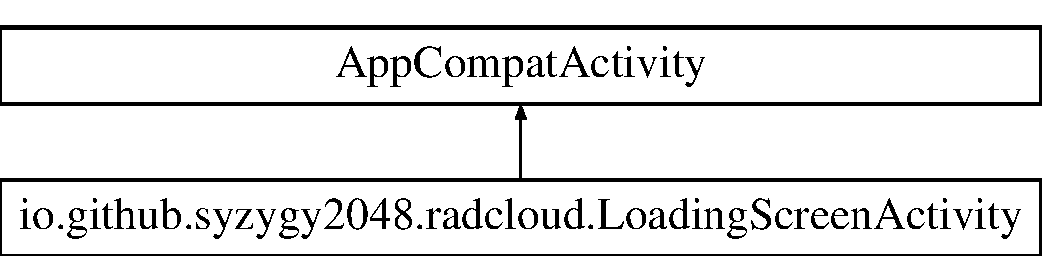
\includegraphics[height=2.000000cm]{classio_1_1github_1_1syzygy2048_1_1radcloud_1_1_loading_screen_activity}
\end{center}
\end{figure}
\subsection*{Protected Member Functions}
\begin{DoxyCompactItemize}
\item 
void \mbox{\hyperlink{classio_1_1github_1_1syzygy2048_1_1radcloud_1_1_loading_screen_activity_a54bc9c6e108e50ba62aff7cc64e812b5}{on\+Create}} (Bundle saved\+Instance\+State)
\end{DoxyCompactItemize}
\subsection*{Private Attributes}
\begin{DoxyCompactItemize}
\item 
final int \mbox{\hyperlink{classio_1_1github_1_1syzygy2048_1_1radcloud_1_1_loading_screen_activity_a8dc1db6478b13139cebca00f957738fd}{W\+A\+I\+T\+\_\+\+T\+I\+ME}} = 2500
\end{DoxyCompactItemize}


\subsection{Member Function Documentation}
\mbox{\Hypertarget{classio_1_1github_1_1syzygy2048_1_1radcloud_1_1_loading_screen_activity_a54bc9c6e108e50ba62aff7cc64e812b5}\label{classio_1_1github_1_1syzygy2048_1_1radcloud_1_1_loading_screen_activity_a54bc9c6e108e50ba62aff7cc64e812b5}} 
\index{io\+::github\+::syzygy2048\+::radcloud\+::\+Loading\+Screen\+Activity@{io\+::github\+::syzygy2048\+::radcloud\+::\+Loading\+Screen\+Activity}!on\+Create@{on\+Create}}
\index{on\+Create@{on\+Create}!io\+::github\+::syzygy2048\+::radcloud\+::\+Loading\+Screen\+Activity@{io\+::github\+::syzygy2048\+::radcloud\+::\+Loading\+Screen\+Activity}}
\subsubsection{\texorpdfstring{on\+Create()}{onCreate()}}
{\footnotesize\ttfamily void io.\+github.\+syzygy2048.\+radcloud.\+Loading\+Screen\+Activity.\+on\+Create (\begin{DoxyParamCaption}\item[{Bundle}]{saved\+Instance\+State }\end{DoxyParamCaption})\hspace{0.3cm}{\ttfamily [protected]}}

Waits until new activity is loaded already 
\begin{DoxyParams}{Parameters}
{\em saved\+Instance\+State} & \\
\hline
\end{DoxyParams}


\subsection{Member Data Documentation}
\mbox{\Hypertarget{classio_1_1github_1_1syzygy2048_1_1radcloud_1_1_loading_screen_activity_a8dc1db6478b13139cebca00f957738fd}\label{classio_1_1github_1_1syzygy2048_1_1radcloud_1_1_loading_screen_activity_a8dc1db6478b13139cebca00f957738fd}} 
\index{io\+::github\+::syzygy2048\+::radcloud\+::\+Loading\+Screen\+Activity@{io\+::github\+::syzygy2048\+::radcloud\+::\+Loading\+Screen\+Activity}!W\+A\+I\+T\+\_\+\+T\+I\+ME@{W\+A\+I\+T\+\_\+\+T\+I\+ME}}
\index{W\+A\+I\+T\+\_\+\+T\+I\+ME@{W\+A\+I\+T\+\_\+\+T\+I\+ME}!io\+::github\+::syzygy2048\+::radcloud\+::\+Loading\+Screen\+Activity@{io\+::github\+::syzygy2048\+::radcloud\+::\+Loading\+Screen\+Activity}}
\subsubsection{\texorpdfstring{W\+A\+I\+T\+\_\+\+T\+I\+ME}{WAIT\_TIME}}
{\footnotesize\ttfamily final int io.\+github.\+syzygy2048.\+radcloud.\+Loading\+Screen\+Activity.\+W\+A\+I\+T\+\_\+\+T\+I\+ME = 2500\hspace{0.3cm}{\ttfamily [private]}}

Delay on opening the new activity 

The documentation for this class was generated from the following file\+:\begin{DoxyCompactItemize}
\item 
C\+:/\+Users/rebeb/\+Documents/\+T\+U Wien/18\+S\+S/\+Info\+Vis/\+U\+E/app/src/main/java/io/github/syzygy2048/radcloud/Loading\+Screen\+Activity.\+java\end{DoxyCompactItemize}

\hypertarget{classio_1_1github_1_1syzygy2048_1_1radcloud_1_1_main_activity}{}\section{io.\+github.\+syzygy2048.\+radcloud.\+Main\+Activity Class Reference}
\label{classio_1_1github_1_1syzygy2048_1_1radcloud_1_1_main_activity}\index{io.\+github.\+syzygy2048.\+radcloud.\+Main\+Activity@{io.\+github.\+syzygy2048.\+radcloud.\+Main\+Activity}}
Inheritance diagram for io.\+github.\+syzygy2048.\+radcloud.\+Main\+Activity\+:\begin{figure}[H]
\begin{center}
\leavevmode
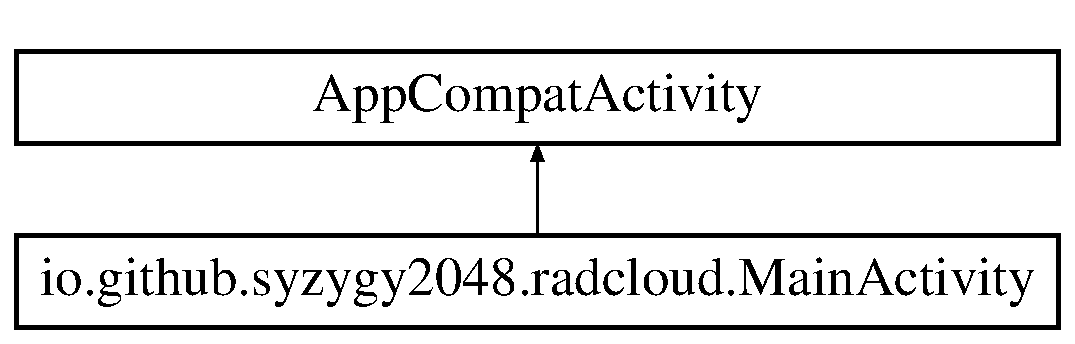
\includegraphics[height=2.000000cm]{classio_1_1github_1_1syzygy2048_1_1radcloud_1_1_main_activity}
\end{center}
\end{figure}
\subsection*{Public Member Functions}
\begin{DoxyCompactItemize}
\item 
void \mbox{\hyperlink{classio_1_1github_1_1syzygy2048_1_1radcloud_1_1_main_activity_aadc64331c63553c85bfc45ce9cee66b2}{on\+Request\+Permissions\+Result}} (int request\+Code, @Non\+Null String\mbox{[}$\,$\mbox{]} permissions, @Non\+Null int\mbox{[}$\,$\mbox{]} grant\+Results)
\end{DoxyCompactItemize}
\subsection*{Protected Member Functions}
\begin{DoxyCompactItemize}
\item 
void \mbox{\hyperlink{classio_1_1github_1_1syzygy2048_1_1radcloud_1_1_main_activity_a3f1dec2ae5371ebbd577d105c8834d74}{on\+Create}} (Bundle saved\+Instance\+State)
\item 
void \mbox{\hyperlink{classio_1_1github_1_1syzygy2048_1_1radcloud_1_1_main_activity_ad31d9aa9ec5da472c81e8b9d4e653bba}{on\+Activity\+Result}} (int request\+Code, int result\+Code, Intent data)
\end{DoxyCompactItemize}


\subsection{Detailed Description}
Entry point for the App. Let\textquotesingle{}s you select and read documents. 

\subsection{Member Function Documentation}
\mbox{\Hypertarget{classio_1_1github_1_1syzygy2048_1_1radcloud_1_1_main_activity_ad31d9aa9ec5da472c81e8b9d4e653bba}\label{classio_1_1github_1_1syzygy2048_1_1radcloud_1_1_main_activity_ad31d9aa9ec5da472c81e8b9d4e653bba}} 
\index{io\+::github\+::syzygy2048\+::radcloud\+::\+Main\+Activity@{io\+::github\+::syzygy2048\+::radcloud\+::\+Main\+Activity}!on\+Activity\+Result@{on\+Activity\+Result}}
\index{on\+Activity\+Result@{on\+Activity\+Result}!io\+::github\+::syzygy2048\+::radcloud\+::\+Main\+Activity@{io\+::github\+::syzygy2048\+::radcloud\+::\+Main\+Activity}}
\subsubsection{\texorpdfstring{on\+Activity\+Result()}{onActivityResult()}}
{\footnotesize\ttfamily void io.\+github.\+syzygy2048.\+radcloud.\+Main\+Activity.\+on\+Activity\+Result (\begin{DoxyParamCaption}\item[{int}]{request\+Code,  }\item[{int}]{result\+Code,  }\item[{Intent}]{data }\end{DoxyParamCaption})\hspace{0.3cm}{\ttfamily [protected]}}

Results of file pickers.


\begin{DoxyParams}{Parameters}
{\em request\+Code} & Request code that was used when starting the file picking. \\
\hline
{\em result\+Code} & A result indicating success of failure. \\
\hline
{\em data} & An intent containing the picked data. \\
\hline
\end{DoxyParams}
\mbox{\Hypertarget{classio_1_1github_1_1syzygy2048_1_1radcloud_1_1_main_activity_a3f1dec2ae5371ebbd577d105c8834d74}\label{classio_1_1github_1_1syzygy2048_1_1radcloud_1_1_main_activity_a3f1dec2ae5371ebbd577d105c8834d74}} 
\index{io\+::github\+::syzygy2048\+::radcloud\+::\+Main\+Activity@{io\+::github\+::syzygy2048\+::radcloud\+::\+Main\+Activity}!on\+Create@{on\+Create}}
\index{on\+Create@{on\+Create}!io\+::github\+::syzygy2048\+::radcloud\+::\+Main\+Activity@{io\+::github\+::syzygy2048\+::radcloud\+::\+Main\+Activity}}
\subsubsection{\texorpdfstring{on\+Create()}{onCreate()}}
{\footnotesize\ttfamily void io.\+github.\+syzygy2048.\+radcloud.\+Main\+Activity.\+on\+Create (\begin{DoxyParamCaption}\item[{Bundle}]{saved\+Instance\+State }\end{DoxyParamCaption})\hspace{0.3cm}{\ttfamily [protected]}}

Create UI structure and define behavior.


\begin{DoxyParams}{Parameters}
{\em saved\+Instance\+State} & -\/ activity properties \\
\hline
\end{DoxyParams}
Start file picker 
\begin{DoxyParams}{Parameters}
{\em v} & clicked button\\
\hline
\end{DoxyParams}
Start file picker 
\begin{DoxyParams}{Parameters}
{\em v} & clicked button\\
\hline
\end{DoxyParams}
Start file picker 
\begin{DoxyParams}{Parameters}
{\em v} & clicked button\\
\hline
\end{DoxyParams}
Start file picker 
\begin{DoxyParams}{Parameters}
{\em v} & clicked button\\
\hline
\end{DoxyParams}
Start file picker 
\begin{DoxyParams}{Parameters}
{\em v} & clicked button\\
\hline
\end{DoxyParams}
Start file picker 
\begin{DoxyParams}{Parameters}
{\em v} & clicked button\\
\hline
\end{DoxyParams}
Read selected files into the document manager for further processing and rendering and start \mbox{\hyperlink{classio_1_1github_1_1syzygy2048_1_1radcloud_1_1_loading_screen_activity}{Loading\+Screen\+Activity}}. 
\begin{DoxyParams}{Parameters}
{\em view} & The clicked view.\\
\hline
\end{DoxyParams}
\mbox{\Hypertarget{classio_1_1github_1_1syzygy2048_1_1radcloud_1_1_main_activity_aadc64331c63553c85bfc45ce9cee66b2}\label{classio_1_1github_1_1syzygy2048_1_1radcloud_1_1_main_activity_aadc64331c63553c85bfc45ce9cee66b2}} 
\index{io\+::github\+::syzygy2048\+::radcloud\+::\+Main\+Activity@{io\+::github\+::syzygy2048\+::radcloud\+::\+Main\+Activity}!on\+Request\+Permissions\+Result@{on\+Request\+Permissions\+Result}}
\index{on\+Request\+Permissions\+Result@{on\+Request\+Permissions\+Result}!io\+::github\+::syzygy2048\+::radcloud\+::\+Main\+Activity@{io\+::github\+::syzygy2048\+::radcloud\+::\+Main\+Activity}}
\subsubsection{\texorpdfstring{on\+Request\+Permissions\+Result()}{onRequestPermissionsResult()}}
{\footnotesize\ttfamily void io.\+github.\+syzygy2048.\+radcloud.\+Main\+Activity.\+on\+Request\+Permissions\+Result (\begin{DoxyParamCaption}\item[{int}]{request\+Code,  }\item[{@Non\+Null String \mbox{[}$\,$\mbox{]}}]{permissions,  }\item[{@Non\+Null int \mbox{[}$\,$\mbox{]}}]{grant\+Results }\end{DoxyParamCaption})}

Gives the result of a permission request. (Write External Memory)


\begin{DoxyParams}{Parameters}
{\em request\+Code} & -\/ Request code that was used when requesting the permission. \\
\hline
{\em permissions} & -\/ Array of requested permissions. \\
\hline
{\em grant\+Results} & -\/ Array of grant results. \\
\hline
\end{DoxyParams}


The documentation for this class was generated from the following file\+:\begin{DoxyCompactItemize}
\item 
C\+:/\+Users/rebeb/\+Documents/\+T\+U Wien/18\+S\+S/\+Info\+Vis/\+U\+E/app/src/main/java/io/github/syzygy2048/radcloud/Main\+Activity.\+java\end{DoxyCompactItemize}

\hypertarget{classio_1_1github_1_1syzygy2048_1_1radcloud_1_1_rad_cloud_activity}{}\section{io.\+github.\+syzygy2048.\+radcloud.\+Rad\+Cloud\+Activity Class Reference}
\label{classio_1_1github_1_1syzygy2048_1_1radcloud_1_1_rad_cloud_activity}\index{io.\+github.\+syzygy2048.\+radcloud.\+Rad\+Cloud\+Activity@{io.\+github.\+syzygy2048.\+radcloud.\+Rad\+Cloud\+Activity}}
Inheritance diagram for io.\+github.\+syzygy2048.\+radcloud.\+Rad\+Cloud\+Activity\+:\begin{figure}[H]
\begin{center}
\leavevmode
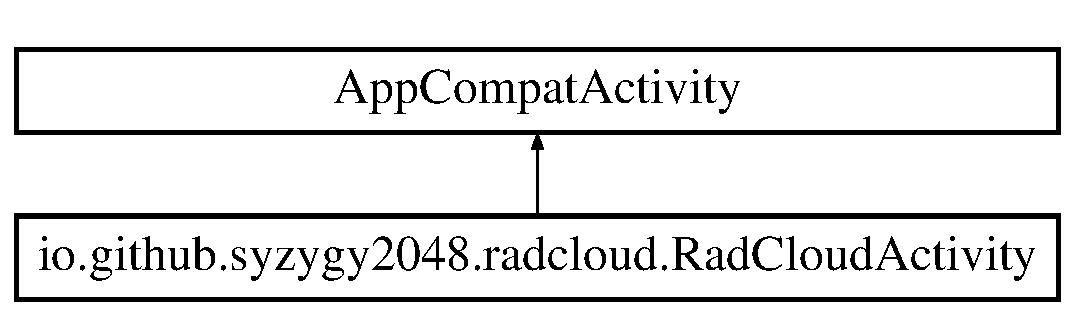
\includegraphics[height=2.000000cm]{classio_1_1github_1_1syzygy2048_1_1radcloud_1_1_rad_cloud_activity}
\end{center}
\end{figure}
\subsection*{Static Public Attributes}
\begin{DoxyCompactItemize}
\item 
static final int \mbox{\hyperlink{classio_1_1github_1_1syzygy2048_1_1radcloud_1_1_rad_cloud_activity_a64bad45183574bf4c3a0af55fe8338f3}{M\+A\+X\+I\+M\+U\+M\+\_\+\+T\+E\+X\+T\+\_\+\+S\+I\+ZE}} = 200
\end{DoxyCompactItemize}
\subsection*{Protected Member Functions}
\begin{DoxyCompactItemize}
\item 
void \mbox{\hyperlink{classio_1_1github_1_1syzygy2048_1_1radcloud_1_1_rad_cloud_activity_a3f26b57f925b135a3242d688b93c9711}{on\+Create}} (Bundle saved\+Instance\+State)
\end{DoxyCompactItemize}
\subsection*{Private Attributes}
\begin{DoxyCompactItemize}
\item 
\mbox{\Hypertarget{classio_1_1github_1_1syzygy2048_1_1radcloud_1_1_rad_cloud_activity_ab18fdc211e7be1230a828c02656d9a0e}\label{classio_1_1github_1_1syzygy2048_1_1radcloud_1_1_rad_cloud_activity_ab18fdc211e7be1230a828c02656d9a0e}} 
Image\+View {\bfseries rad\+Cloud\+View}
\end{DoxyCompactItemize}


\subsection{Detailed Description}
Fullscreen activity used to render the Rad\+Cloud. 

\subsection{Member Function Documentation}
\mbox{\Hypertarget{classio_1_1github_1_1syzygy2048_1_1radcloud_1_1_rad_cloud_activity_a3f26b57f925b135a3242d688b93c9711}\label{classio_1_1github_1_1syzygy2048_1_1radcloud_1_1_rad_cloud_activity_a3f26b57f925b135a3242d688b93c9711}} 
\index{io\+::github\+::syzygy2048\+::radcloud\+::\+Rad\+Cloud\+Activity@{io\+::github\+::syzygy2048\+::radcloud\+::\+Rad\+Cloud\+Activity}!on\+Create@{on\+Create}}
\index{on\+Create@{on\+Create}!io\+::github\+::syzygy2048\+::radcloud\+::\+Rad\+Cloud\+Activity@{io\+::github\+::syzygy2048\+::radcloud\+::\+Rad\+Cloud\+Activity}}
\subsubsection{\texorpdfstring{on\+Create()}{onCreate()}}
{\footnotesize\ttfamily void io.\+github.\+syzygy2048.\+radcloud.\+Rad\+Cloud\+Activity.\+on\+Create (\begin{DoxyParamCaption}\item[{Bundle}]{saved\+Instance\+State }\end{DoxyParamCaption})\hspace{0.3cm}{\ttfamily [protected]}}

Draws the Rad\+Cloud and displays it on screen. 
\begin{DoxyParams}{Parameters}
{\em saved\+Instance\+State} & -\/ default android behavior \\
\hline
\end{DoxyParams}


\subsection{Member Data Documentation}
\mbox{\Hypertarget{classio_1_1github_1_1syzygy2048_1_1radcloud_1_1_rad_cloud_activity_a64bad45183574bf4c3a0af55fe8338f3}\label{classio_1_1github_1_1syzygy2048_1_1radcloud_1_1_rad_cloud_activity_a64bad45183574bf4c3a0af55fe8338f3}} 
\index{io\+::github\+::syzygy2048\+::radcloud\+::\+Rad\+Cloud\+Activity@{io\+::github\+::syzygy2048\+::radcloud\+::\+Rad\+Cloud\+Activity}!M\+A\+X\+I\+M\+U\+M\+\_\+\+T\+E\+X\+T\+\_\+\+S\+I\+ZE@{M\+A\+X\+I\+M\+U\+M\+\_\+\+T\+E\+X\+T\+\_\+\+S\+I\+ZE}}
\index{M\+A\+X\+I\+M\+U\+M\+\_\+\+T\+E\+X\+T\+\_\+\+S\+I\+ZE@{M\+A\+X\+I\+M\+U\+M\+\_\+\+T\+E\+X\+T\+\_\+\+S\+I\+ZE}!io\+::github\+::syzygy2048\+::radcloud\+::\+Rad\+Cloud\+Activity@{io\+::github\+::syzygy2048\+::radcloud\+::\+Rad\+Cloud\+Activity}}
\subsubsection{\texorpdfstring{M\+A\+X\+I\+M\+U\+M\+\_\+\+T\+E\+X\+T\+\_\+\+S\+I\+ZE}{MAXIMUM\_TEXT\_SIZE}}
{\footnotesize\ttfamily final int io.\+github.\+syzygy2048.\+radcloud.\+Rad\+Cloud\+Activity.\+M\+A\+X\+I\+M\+U\+M\+\_\+\+T\+E\+X\+T\+\_\+\+S\+I\+ZE = 200\hspace{0.3cm}{\ttfamily [static]}}

The maximum size a text can have. 

The documentation for this class was generated from the following file\+:\begin{DoxyCompactItemize}
\item 
C\+:/\+Users/rebeb/\+Documents/\+T\+U Wien/18\+S\+S/\+Info\+Vis/\+U\+E/app/src/main/java/io/github/syzygy2048/radcloud/Rad\+Cloud\+Activity.\+java\end{DoxyCompactItemize}

\hypertarget{classio_1_1github_1_1syzygy2048_1_1radcloud_1_1_spiral_generator}{}\section{io.\+github.\+syzygy2048.\+radcloud.\+Spiral\+Generator Class Reference}
\label{classio_1_1github_1_1syzygy2048_1_1radcloud_1_1_spiral_generator}\index{io.\+github.\+syzygy2048.\+radcloud.\+Spiral\+Generator@{io.\+github.\+syzygy2048.\+radcloud.\+Spiral\+Generator}}
\subsection*{Static Public Member Functions}
\begin{DoxyCompactItemize}
\item 
static Document\+Manager.\+Vec2 \mbox{\hyperlink{classio_1_1github_1_1syzygy2048_1_1radcloud_1_1_spiral_generator_afecbb70e7e893866ce0bf01260734f5e}{calculate\+Spiral}} (int iteration)
\end{DoxyCompactItemize}


\subsection{Detailed Description}
This class is used to equidistant points on a spiral. Based on\+: \href{https://stackoverflow.com/questions/13894715/draw-equidistant-points-on-a-spiral}{\tt https\+://stackoverflow.\+com/questions/13894715/draw-\/equidistant-\/points-\/on-\/a-\/spiral} 

\subsection{Member Function Documentation}
\mbox{\Hypertarget{classio_1_1github_1_1syzygy2048_1_1radcloud_1_1_spiral_generator_afecbb70e7e893866ce0bf01260734f5e}\label{classio_1_1github_1_1syzygy2048_1_1radcloud_1_1_spiral_generator_afecbb70e7e893866ce0bf01260734f5e}} 
\index{io\+::github\+::syzygy2048\+::radcloud\+::\+Spiral\+Generator@{io\+::github\+::syzygy2048\+::radcloud\+::\+Spiral\+Generator}!calculate\+Spiral@{calculate\+Spiral}}
\index{calculate\+Spiral@{calculate\+Spiral}!io\+::github\+::syzygy2048\+::radcloud\+::\+Spiral\+Generator@{io\+::github\+::syzygy2048\+::radcloud\+::\+Spiral\+Generator}}
\subsubsection{\texorpdfstring{calculate\+Spiral()}{calculateSpiral()}}
{\footnotesize\ttfamily static Document\+Manager.\+Vec2 io.\+github.\+syzygy2048.\+radcloud.\+Spiral\+Generator.\+calculate\+Spiral (\begin{DoxyParamCaption}\item[{int}]{iteration }\end{DoxyParamCaption})\hspace{0.3cm}{\ttfamily [inline]}, {\ttfamily [static]}}

Calculate an return a single point on an equidistant spiral. The points are equidistant and move outwarsd along the coils from the center (0/0).


\begin{DoxyParams}{Parameters}
{\em iteration} & -\/ indicates how many points removed from the center the point should be calculated at. \\
\hline
\end{DoxyParams}
\begin{DoxyReturn}{Returns}
\mbox{\hyperlink{classio_1_1github_1_1syzygy2048_1_1radcloud_1_1_document_manager_1_1_vec2}{Document\+Manager.\+Vec2}} -\/ The x/y coordinates of the calculates point. 
\end{DoxyReturn}


The documentation for this class was generated from the following file\+:\begin{DoxyCompactItemize}
\item 
C\+:/\+Users/rebeb/\+Documents/\+T\+U Wien/18\+S\+S/\+Info\+Vis/\+U\+E/app/src/main/java/io/github/syzygy2048/radcloud/Spiral\+Generator.\+java\end{DoxyCompactItemize}

\hypertarget{classio_1_1github_1_1syzygy2048_1_1radcloud_1_1_document_manager_1_1_vec2}{}\section{io.\+github.\+syzygy2048.\+radcloud.\+Document\+Manager.\+Vec2 Class Reference}
\label{classio_1_1github_1_1syzygy2048_1_1radcloud_1_1_document_manager_1_1_vec2}\index{io.\+github.\+syzygy2048.\+radcloud.\+Document\+Manager.\+Vec2@{io.\+github.\+syzygy2048.\+radcloud.\+Document\+Manager.\+Vec2}}


\subsection{Detailed Description}
Class for a 2D vector 

The documentation for this class was generated from the following file\+:\begin{DoxyCompactItemize}
\item 
C\+:/\+Users/rebeb/\+Documents/\+T\+U Wien/18\+S\+S/\+Info\+Vis/\+U\+E/app/src/main/java/io/github/syzygy2048/radcloud/Document\+Manager.\+java\end{DoxyCompactItemize}

\hypertarget{classio_1_1github_1_1syzygy2048_1_1radcloud_1_1_word}{}\section{io.\+github.\+syzygy2048.\+radcloud.\+Word Class Reference}
\label{classio_1_1github_1_1syzygy2048_1_1radcloud_1_1_word}\index{io.\+github.\+syzygy2048.\+radcloud.\+Word@{io.\+github.\+syzygy2048.\+radcloud.\+Word}}
\subsection*{Public Member Functions}
\begin{DoxyCompactItemize}
\item 
float \mbox{\hyperlink{classio_1_1github_1_1syzygy2048_1_1radcloud_1_1_word_a650b6f0273d5d3506f011c755ceb0c2b}{get\+Maximum\+Relevance}} ()
\item 
void \mbox{\hyperlink{classio_1_1github_1_1syzygy2048_1_1radcloud_1_1_word_a8b1e2ce149323bdcabc97acd475ada03}{set\+Maximum\+Relevance}} (float \mbox{\hyperlink{classio_1_1github_1_1syzygy2048_1_1radcloud_1_1_word_aed758b7df9156075124f25815df3f045}{maximum\+Relevance}})
\item 
Hash\+Map$<$ String, Float $>$ \mbox{\hyperlink{classio_1_1github_1_1syzygy2048_1_1radcloud_1_1_word_a43d025c6b84e26e43d860e2039b038b3}{get\+Category\+Weights}} ()
\item 
void \mbox{\hyperlink{classio_1_1github_1_1syzygy2048_1_1radcloud_1_1_word_ad9cc049a275474fb0e07f6936a4f0482}{set\+Category\+Weights}} (Hash\+Map$<$ String, Float $>$ \mbox{\hyperlink{classio_1_1github_1_1syzygy2048_1_1radcloud_1_1_word_ad698485d567053d6752dbec826506744}{category\+Weights}})
\item 
Hash\+Map$<$ String, Float $>$ \mbox{\hyperlink{classio_1_1github_1_1syzygy2048_1_1radcloud_1_1_word_a2ee90d130c2dfc37098cb4e054ca0543}{get\+Placement\+Weights}} ()
\item 
void \mbox{\hyperlink{classio_1_1github_1_1syzygy2048_1_1radcloud_1_1_word_a01c894a4b416e7ec5aad897665d43760}{set\+Placement\+Weights}} (Hash\+Map$<$ String, Float $>$ \mbox{\hyperlink{classio_1_1github_1_1syzygy2048_1_1radcloud_1_1_word_a8023b6dc40adf585ad20ba73ab237bab}{placement\+Weights}})
\item 
String \mbox{\hyperlink{classio_1_1github_1_1syzygy2048_1_1radcloud_1_1_word_a7e81adc8a7bcf0b31ab23629bed42a9a}{get\+Term}} ()
\item 
Hash\+Map$<$ String, Float $>$ \mbox{\hyperlink{classio_1_1github_1_1syzygy2048_1_1radcloud_1_1_word_ae834f3cc726881ca956767761d82910b}{get\+Term\+Frequency}} ()
\item 
Hash\+Map$<$ String, Integer $>$ \mbox{\hyperlink{classio_1_1github_1_1syzygy2048_1_1radcloud_1_1_word_ad8eee7d4d1d7b307312855b069dbe5cd}{get\+Word\+Count}} ()
\item 
void \mbox{\hyperlink{classio_1_1github_1_1syzygy2048_1_1radcloud_1_1_word_af55e8190330dd775ea153fee1750176a}{set\+Term\+Frequency}} (Hash\+Map$<$ String, Float $>$ tf)
\item 
void \mbox{\hyperlink{classio_1_1github_1_1syzygy2048_1_1radcloud_1_1_word_a234e5e329ae68e4026a09ddeed7945bf}{set\+Inverse\+Document\+Frequency}} (float idf)
\item 
float \mbox{\hyperlink{classio_1_1github_1_1syzygy2048_1_1radcloud_1_1_word_a1b4a8a0ca776c16a5f2192f59f2974b3}{get\+Inverse\+Document\+Frequency}} ()
\item 
boolean \mbox{\hyperlink{classio_1_1github_1_1syzygy2048_1_1radcloud_1_1_word_ad35bce76832c85b100a4346da0f20a00}{equals}} (Object obj)
\item 
void \mbox{\hyperlink{classio_1_1github_1_1syzygy2048_1_1radcloud_1_1_word_a493351b57cf532161237dd873509f79d}{set\+Normalized\+Weights}} (Hash\+Map$<$ String, Float $>$ \mbox{\hyperlink{classio_1_1github_1_1syzygy2048_1_1radcloud_1_1_word_a73284999ac4b313793306806096f6a86}{normalized\+Weights}})
\item 
Hash\+Map$<$ String, Float $>$ \mbox{\hyperlink{classio_1_1github_1_1syzygy2048_1_1radcloud_1_1_word_aee98861b9717bf6e3a013b0d4d5bf3c4}{get\+Normalized\+Weights}} ()
\item 
void \mbox{\hyperlink{classio_1_1github_1_1syzygy2048_1_1radcloud_1_1_word_a0032169550f9764ce15473b5043e6d59}{set\+Intended\+Position}} (Document\+Manager.\+Vec2 \mbox{\hyperlink{classio_1_1github_1_1syzygy2048_1_1radcloud_1_1_word_a064f2f7f9b0e939fe3b2cfd2cc87817f}{intended\+Position}})
\item 
Document\+Manager.\+Vec2 \mbox{\hyperlink{classio_1_1github_1_1syzygy2048_1_1radcloud_1_1_word_a5e03f2a9bb4acf21a8e991b060126994}{get\+Position}} ()
\item 
void \mbox{\hyperlink{classio_1_1github_1_1syzygy2048_1_1radcloud_1_1_word_a47529581dc9d3302b054c7a33981c375}{calculate\+Bounding\+Box}} (float \mbox{\hyperlink{classio_1_1github_1_1syzygy2048_1_1radcloud_1_1_word_aed758b7df9156075124f25815df3f045}{maximum\+Relevance}})
\item 
void \mbox{\hyperlink{classio_1_1github_1_1syzygy2048_1_1radcloud_1_1_word_a3bd7b70cf654bbe3c0f6db2bfbaf0929}{calculate\+Bounding\+Box}} (Paint paint, float maximum\+Word\+Relevance)
\end{DoxyCompactItemize}
\subsection*{Private Attributes}
\begin{DoxyCompactItemize}
\item 
String \mbox{\hyperlink{classio_1_1github_1_1syzygy2048_1_1radcloud_1_1_word_a6315b33ceb56892c35cf85ba006bb404}{term}}
\item 
Hash\+Map$<$ String, Float $>$ \mbox{\hyperlink{classio_1_1github_1_1syzygy2048_1_1radcloud_1_1_word_afd48720786b3805982c8afbc8b2e182e}{term\+Frequency}} = new Hash\+Map$<$$>$()
\item 
Hash\+Map$<$ String, Integer $>$ \mbox{\hyperlink{classio_1_1github_1_1syzygy2048_1_1radcloud_1_1_word_acabb157342af2ce8233ecfa0061dfc08}{count\+By\+Document}} = new Hash\+Map$<$$>$()
\item 
float \mbox{\hyperlink{classio_1_1github_1_1syzygy2048_1_1radcloud_1_1_word_a7e900346d6a4ce49783a11c9dac7ee57}{inverse\+Document\+Frequency}}
\item 
Hash\+Map$<$ String, Float $>$ \mbox{\hyperlink{classio_1_1github_1_1syzygy2048_1_1radcloud_1_1_word_a73284999ac4b313793306806096f6a86}{normalized\+Weights}}
\item 
Hash\+Map$<$ String, Float $>$ \mbox{\hyperlink{classio_1_1github_1_1syzygy2048_1_1radcloud_1_1_word_ad698485d567053d6752dbec826506744}{category\+Weights}}
\item 
Hash\+Map$<$ String, Float $>$ \mbox{\hyperlink{classio_1_1github_1_1syzygy2048_1_1radcloud_1_1_word_a8023b6dc40adf585ad20ba73ab237bab}{placement\+Weights}}
\item 
Document\+Manager.\+Vec2 \mbox{\hyperlink{classio_1_1github_1_1syzygy2048_1_1radcloud_1_1_word_a064f2f7f9b0e939fe3b2cfd2cc87817f}{intended\+Position}}
\item 
float \mbox{\hyperlink{classio_1_1github_1_1syzygy2048_1_1radcloud_1_1_word_aed758b7df9156075124f25815df3f045}{maximum\+Relevance}}
\end{DoxyCompactItemize}


\subsection{Detailed Description}
Created by rebeb on 5/8/2018. 

\subsection{Member Function Documentation}
\mbox{\Hypertarget{classio_1_1github_1_1syzygy2048_1_1radcloud_1_1_word_a47529581dc9d3302b054c7a33981c375}\label{classio_1_1github_1_1syzygy2048_1_1radcloud_1_1_word_a47529581dc9d3302b054c7a33981c375}} 
\index{io\+::github\+::syzygy2048\+::radcloud\+::\+Word@{io\+::github\+::syzygy2048\+::radcloud\+::\+Word}!calculate\+Bounding\+Box@{calculate\+Bounding\+Box}}
\index{calculate\+Bounding\+Box@{calculate\+Bounding\+Box}!io\+::github\+::syzygy2048\+::radcloud\+::\+Word@{io\+::github\+::syzygy2048\+::radcloud\+::\+Word}}
\subsubsection{\texorpdfstring{calculate\+Bounding\+Box()}{calculateBoundingBox()}\hspace{0.1cm}{\footnotesize\ttfamily [1/2]}}
{\footnotesize\ttfamily void io.\+github.\+syzygy2048.\+radcloud.\+Word.\+calculate\+Bounding\+Box (\begin{DoxyParamCaption}\item[{float}]{maximum\+Relevance }\end{DoxyParamCaption})}

calculates the bounding box of the word 
\begin{DoxyParams}{Parameters}
{\em maximum\+Relevance} & \\
\hline
\end{DoxyParams}
\mbox{\Hypertarget{classio_1_1github_1_1syzygy2048_1_1radcloud_1_1_word_a3bd7b70cf654bbe3c0f6db2bfbaf0929}\label{classio_1_1github_1_1syzygy2048_1_1radcloud_1_1_word_a3bd7b70cf654bbe3c0f6db2bfbaf0929}} 
\index{io\+::github\+::syzygy2048\+::radcloud\+::\+Word@{io\+::github\+::syzygy2048\+::radcloud\+::\+Word}!calculate\+Bounding\+Box@{calculate\+Bounding\+Box}}
\index{calculate\+Bounding\+Box@{calculate\+Bounding\+Box}!io\+::github\+::syzygy2048\+::radcloud\+::\+Word@{io\+::github\+::syzygy2048\+::radcloud\+::\+Word}}
\subsubsection{\texorpdfstring{calculate\+Bounding\+Box()}{calculateBoundingBox()}\hspace{0.1cm}{\footnotesize\ttfamily [2/2]}}
{\footnotesize\ttfamily void io.\+github.\+syzygy2048.\+radcloud.\+Word.\+calculate\+Bounding\+Box (\begin{DoxyParamCaption}\item[{Paint}]{paint,  }\item[{float}]{maximum\+Word\+Relevance }\end{DoxyParamCaption})}

Calculates the bounding box according to word size 
\begin{DoxyParams}{Parameters}
{\em paint} & \\
\hline
{\em maximum\+Word\+Relevance} & \\
\hline
\end{DoxyParams}
\mbox{\Hypertarget{classio_1_1github_1_1syzygy2048_1_1radcloud_1_1_word_ad35bce76832c85b100a4346da0f20a00}\label{classio_1_1github_1_1syzygy2048_1_1radcloud_1_1_word_ad35bce76832c85b100a4346da0f20a00}} 
\index{io\+::github\+::syzygy2048\+::radcloud\+::\+Word@{io\+::github\+::syzygy2048\+::radcloud\+::\+Word}!equals@{equals}}
\index{equals@{equals}!io\+::github\+::syzygy2048\+::radcloud\+::\+Word@{io\+::github\+::syzygy2048\+::radcloud\+::\+Word}}
\subsubsection{\texorpdfstring{equals()}{equals()}}
{\footnotesize\ttfamily boolean io.\+github.\+syzygy2048.\+radcloud.\+Word.\+equals (\begin{DoxyParamCaption}\item[{Object}]{obj }\end{DoxyParamCaption})}

Compares two words 
\begin{DoxyParams}{Parameters}
{\em obj} & word to compare \\
\hline
\end{DoxyParams}
\begin{DoxyReturn}{Returns}

\end{DoxyReturn}
\mbox{\Hypertarget{classio_1_1github_1_1syzygy2048_1_1radcloud_1_1_word_a43d025c6b84e26e43d860e2039b038b3}\label{classio_1_1github_1_1syzygy2048_1_1radcloud_1_1_word_a43d025c6b84e26e43d860e2039b038b3}} 
\index{io\+::github\+::syzygy2048\+::radcloud\+::\+Word@{io\+::github\+::syzygy2048\+::radcloud\+::\+Word}!get\+Category\+Weights@{get\+Category\+Weights}}
\index{get\+Category\+Weights@{get\+Category\+Weights}!io\+::github\+::syzygy2048\+::radcloud\+::\+Word@{io\+::github\+::syzygy2048\+::radcloud\+::\+Word}}
\subsubsection{\texorpdfstring{get\+Category\+Weights()}{getCategoryWeights()}}
{\footnotesize\ttfamily Hash\+Map$<$String, Float$>$ io.\+github.\+syzygy2048.\+radcloud.\+Word.\+get\+Category\+Weights (\begin{DoxyParamCaption}{ }\end{DoxyParamCaption})}

getter for category weights \begin{DoxyReturn}{Returns}
category weights 
\end{DoxyReturn}
\mbox{\Hypertarget{classio_1_1github_1_1syzygy2048_1_1radcloud_1_1_word_a1b4a8a0ca776c16a5f2192f59f2974b3}\label{classio_1_1github_1_1syzygy2048_1_1radcloud_1_1_word_a1b4a8a0ca776c16a5f2192f59f2974b3}} 
\index{io\+::github\+::syzygy2048\+::radcloud\+::\+Word@{io\+::github\+::syzygy2048\+::radcloud\+::\+Word}!get\+Inverse\+Document\+Frequency@{get\+Inverse\+Document\+Frequency}}
\index{get\+Inverse\+Document\+Frequency@{get\+Inverse\+Document\+Frequency}!io\+::github\+::syzygy2048\+::radcloud\+::\+Word@{io\+::github\+::syzygy2048\+::radcloud\+::\+Word}}
\subsubsection{\texorpdfstring{get\+Inverse\+Document\+Frequency()}{getInverseDocumentFrequency()}}
{\footnotesize\ttfamily float io.\+github.\+syzygy2048.\+radcloud.\+Word.\+get\+Inverse\+Document\+Frequency (\begin{DoxyParamCaption}{ }\end{DoxyParamCaption})}

getter for inverse document ferquency \begin{DoxyReturn}{Returns}

\end{DoxyReturn}
\mbox{\Hypertarget{classio_1_1github_1_1syzygy2048_1_1radcloud_1_1_word_a650b6f0273d5d3506f011c755ceb0c2b}\label{classio_1_1github_1_1syzygy2048_1_1radcloud_1_1_word_a650b6f0273d5d3506f011c755ceb0c2b}} 
\index{io\+::github\+::syzygy2048\+::radcloud\+::\+Word@{io\+::github\+::syzygy2048\+::radcloud\+::\+Word}!get\+Maximum\+Relevance@{get\+Maximum\+Relevance}}
\index{get\+Maximum\+Relevance@{get\+Maximum\+Relevance}!io\+::github\+::syzygy2048\+::radcloud\+::\+Word@{io\+::github\+::syzygy2048\+::radcloud\+::\+Word}}
\subsubsection{\texorpdfstring{get\+Maximum\+Relevance()}{getMaximumRelevance()}}
{\footnotesize\ttfamily float io.\+github.\+syzygy2048.\+radcloud.\+Word.\+get\+Maximum\+Relevance (\begin{DoxyParamCaption}{ }\end{DoxyParamCaption})}

getter for maximum relevance \begin{DoxyReturn}{Returns}
maximum relevance 
\end{DoxyReturn}
\mbox{\Hypertarget{classio_1_1github_1_1syzygy2048_1_1radcloud_1_1_word_aee98861b9717bf6e3a013b0d4d5bf3c4}\label{classio_1_1github_1_1syzygy2048_1_1radcloud_1_1_word_aee98861b9717bf6e3a013b0d4d5bf3c4}} 
\index{io\+::github\+::syzygy2048\+::radcloud\+::\+Word@{io\+::github\+::syzygy2048\+::radcloud\+::\+Word}!get\+Normalized\+Weights@{get\+Normalized\+Weights}}
\index{get\+Normalized\+Weights@{get\+Normalized\+Weights}!io\+::github\+::syzygy2048\+::radcloud\+::\+Word@{io\+::github\+::syzygy2048\+::radcloud\+::\+Word}}
\subsubsection{\texorpdfstring{get\+Normalized\+Weights()}{getNormalizedWeights()}}
{\footnotesize\ttfamily Hash\+Map$<$String, Float$>$ io.\+github.\+syzygy2048.\+radcloud.\+Word.\+get\+Normalized\+Weights (\begin{DoxyParamCaption}{ }\end{DoxyParamCaption})}

getter for normalized weights \begin{DoxyReturn}{Returns}

\end{DoxyReturn}
\mbox{\Hypertarget{classio_1_1github_1_1syzygy2048_1_1radcloud_1_1_word_a2ee90d130c2dfc37098cb4e054ca0543}\label{classio_1_1github_1_1syzygy2048_1_1radcloud_1_1_word_a2ee90d130c2dfc37098cb4e054ca0543}} 
\index{io\+::github\+::syzygy2048\+::radcloud\+::\+Word@{io\+::github\+::syzygy2048\+::radcloud\+::\+Word}!get\+Placement\+Weights@{get\+Placement\+Weights}}
\index{get\+Placement\+Weights@{get\+Placement\+Weights}!io\+::github\+::syzygy2048\+::radcloud\+::\+Word@{io\+::github\+::syzygy2048\+::radcloud\+::\+Word}}
\subsubsection{\texorpdfstring{get\+Placement\+Weights()}{getPlacementWeights()}}
{\footnotesize\ttfamily Hash\+Map$<$String, Float$>$ io.\+github.\+syzygy2048.\+radcloud.\+Word.\+get\+Placement\+Weights (\begin{DoxyParamCaption}{ }\end{DoxyParamCaption})}

getter for placement weights \begin{DoxyReturn}{Returns}

\end{DoxyReturn}
\mbox{\Hypertarget{classio_1_1github_1_1syzygy2048_1_1radcloud_1_1_word_a5e03f2a9bb4acf21a8e991b060126994}\label{classio_1_1github_1_1syzygy2048_1_1radcloud_1_1_word_a5e03f2a9bb4acf21a8e991b060126994}} 
\index{io\+::github\+::syzygy2048\+::radcloud\+::\+Word@{io\+::github\+::syzygy2048\+::radcloud\+::\+Word}!get\+Position@{get\+Position}}
\index{get\+Position@{get\+Position}!io\+::github\+::syzygy2048\+::radcloud\+::\+Word@{io\+::github\+::syzygy2048\+::radcloud\+::\+Word}}
\subsubsection{\texorpdfstring{get\+Position()}{getPosition()}}
{\footnotesize\ttfamily Document\+Manager.\+Vec2 io.\+github.\+syzygy2048.\+radcloud.\+Word.\+get\+Position (\begin{DoxyParamCaption}{ }\end{DoxyParamCaption})}

getter for word position \begin{DoxyReturn}{Returns}

\end{DoxyReturn}
\mbox{\Hypertarget{classio_1_1github_1_1syzygy2048_1_1radcloud_1_1_word_a7e81adc8a7bcf0b31ab23629bed42a9a}\label{classio_1_1github_1_1syzygy2048_1_1radcloud_1_1_word_a7e81adc8a7bcf0b31ab23629bed42a9a}} 
\index{io\+::github\+::syzygy2048\+::radcloud\+::\+Word@{io\+::github\+::syzygy2048\+::radcloud\+::\+Word}!get\+Term@{get\+Term}}
\index{get\+Term@{get\+Term}!io\+::github\+::syzygy2048\+::radcloud\+::\+Word@{io\+::github\+::syzygy2048\+::radcloud\+::\+Word}}
\subsubsection{\texorpdfstring{get\+Term()}{getTerm()}}
{\footnotesize\ttfamily String io.\+github.\+syzygy2048.\+radcloud.\+Word.\+get\+Term (\begin{DoxyParamCaption}{ }\end{DoxyParamCaption})}

getter for term \begin{DoxyReturn}{Returns}

\end{DoxyReturn}
\mbox{\Hypertarget{classio_1_1github_1_1syzygy2048_1_1radcloud_1_1_word_ae834f3cc726881ca956767761d82910b}\label{classio_1_1github_1_1syzygy2048_1_1radcloud_1_1_word_ae834f3cc726881ca956767761d82910b}} 
\index{io\+::github\+::syzygy2048\+::radcloud\+::\+Word@{io\+::github\+::syzygy2048\+::radcloud\+::\+Word}!get\+Term\+Frequency@{get\+Term\+Frequency}}
\index{get\+Term\+Frequency@{get\+Term\+Frequency}!io\+::github\+::syzygy2048\+::radcloud\+::\+Word@{io\+::github\+::syzygy2048\+::radcloud\+::\+Word}}
\subsubsection{\texorpdfstring{get\+Term\+Frequency()}{getTermFrequency()}}
{\footnotesize\ttfamily Hash\+Map$<$String, Float$>$ io.\+github.\+syzygy2048.\+radcloud.\+Word.\+get\+Term\+Frequency (\begin{DoxyParamCaption}{ }\end{DoxyParamCaption})}

getter for term frequency \begin{DoxyReturn}{Returns}

\end{DoxyReturn}
\mbox{\Hypertarget{classio_1_1github_1_1syzygy2048_1_1radcloud_1_1_word_ad8eee7d4d1d7b307312855b069dbe5cd}\label{classio_1_1github_1_1syzygy2048_1_1radcloud_1_1_word_ad8eee7d4d1d7b307312855b069dbe5cd}} 
\index{io\+::github\+::syzygy2048\+::radcloud\+::\+Word@{io\+::github\+::syzygy2048\+::radcloud\+::\+Word}!get\+Word\+Count@{get\+Word\+Count}}
\index{get\+Word\+Count@{get\+Word\+Count}!io\+::github\+::syzygy2048\+::radcloud\+::\+Word@{io\+::github\+::syzygy2048\+::radcloud\+::\+Word}}
\subsubsection{\texorpdfstring{get\+Word\+Count()}{getWordCount()}}
{\footnotesize\ttfamily Hash\+Map$<$String, Integer$>$ io.\+github.\+syzygy2048.\+radcloud.\+Word.\+get\+Word\+Count (\begin{DoxyParamCaption}{ }\end{DoxyParamCaption})}

getter for word occurances \begin{DoxyReturn}{Returns}

\end{DoxyReturn}
\mbox{\Hypertarget{classio_1_1github_1_1syzygy2048_1_1radcloud_1_1_word_ad9cc049a275474fb0e07f6936a4f0482}\label{classio_1_1github_1_1syzygy2048_1_1radcloud_1_1_word_ad9cc049a275474fb0e07f6936a4f0482}} 
\index{io\+::github\+::syzygy2048\+::radcloud\+::\+Word@{io\+::github\+::syzygy2048\+::radcloud\+::\+Word}!set\+Category\+Weights@{set\+Category\+Weights}}
\index{set\+Category\+Weights@{set\+Category\+Weights}!io\+::github\+::syzygy2048\+::radcloud\+::\+Word@{io\+::github\+::syzygy2048\+::radcloud\+::\+Word}}
\subsubsection{\texorpdfstring{set\+Category\+Weights()}{setCategoryWeights()}}
{\footnotesize\ttfamily void io.\+github.\+syzygy2048.\+radcloud.\+Word.\+set\+Category\+Weights (\begin{DoxyParamCaption}\item[{Hash\+Map$<$ String, Float $>$}]{category\+Weights }\end{DoxyParamCaption})}

setter for category weights 
\begin{DoxyParams}{Parameters}
{\em category\+Weights} & \\
\hline
\end{DoxyParams}
\mbox{\Hypertarget{classio_1_1github_1_1syzygy2048_1_1radcloud_1_1_word_a0032169550f9764ce15473b5043e6d59}\label{classio_1_1github_1_1syzygy2048_1_1radcloud_1_1_word_a0032169550f9764ce15473b5043e6d59}} 
\index{io\+::github\+::syzygy2048\+::radcloud\+::\+Word@{io\+::github\+::syzygy2048\+::radcloud\+::\+Word}!set\+Intended\+Position@{set\+Intended\+Position}}
\index{set\+Intended\+Position@{set\+Intended\+Position}!io\+::github\+::syzygy2048\+::radcloud\+::\+Word@{io\+::github\+::syzygy2048\+::radcloud\+::\+Word}}
\subsubsection{\texorpdfstring{set\+Intended\+Position()}{setIntendedPosition()}}
{\footnotesize\ttfamily void io.\+github.\+syzygy2048.\+radcloud.\+Word.\+set\+Intended\+Position (\begin{DoxyParamCaption}\item[{Document\+Manager.\+Vec2}]{intended\+Position }\end{DoxyParamCaption})}

setter for intended position 
\begin{DoxyParams}{Parameters}
{\em intended\+Position} & \\
\hline
\end{DoxyParams}
\mbox{\Hypertarget{classio_1_1github_1_1syzygy2048_1_1radcloud_1_1_word_a234e5e329ae68e4026a09ddeed7945bf}\label{classio_1_1github_1_1syzygy2048_1_1radcloud_1_1_word_a234e5e329ae68e4026a09ddeed7945bf}} 
\index{io\+::github\+::syzygy2048\+::radcloud\+::\+Word@{io\+::github\+::syzygy2048\+::radcloud\+::\+Word}!set\+Inverse\+Document\+Frequency@{set\+Inverse\+Document\+Frequency}}
\index{set\+Inverse\+Document\+Frequency@{set\+Inverse\+Document\+Frequency}!io\+::github\+::syzygy2048\+::radcloud\+::\+Word@{io\+::github\+::syzygy2048\+::radcloud\+::\+Word}}
\subsubsection{\texorpdfstring{set\+Inverse\+Document\+Frequency()}{setInverseDocumentFrequency()}}
{\footnotesize\ttfamily void io.\+github.\+syzygy2048.\+radcloud.\+Word.\+set\+Inverse\+Document\+Frequency (\begin{DoxyParamCaption}\item[{float}]{idf }\end{DoxyParamCaption})}

setter for inverse document frequency 
\begin{DoxyParams}{Parameters}
{\em idf} & \\
\hline
\end{DoxyParams}
\mbox{\Hypertarget{classio_1_1github_1_1syzygy2048_1_1radcloud_1_1_word_a8b1e2ce149323bdcabc97acd475ada03}\label{classio_1_1github_1_1syzygy2048_1_1radcloud_1_1_word_a8b1e2ce149323bdcabc97acd475ada03}} 
\index{io\+::github\+::syzygy2048\+::radcloud\+::\+Word@{io\+::github\+::syzygy2048\+::radcloud\+::\+Word}!set\+Maximum\+Relevance@{set\+Maximum\+Relevance}}
\index{set\+Maximum\+Relevance@{set\+Maximum\+Relevance}!io\+::github\+::syzygy2048\+::radcloud\+::\+Word@{io\+::github\+::syzygy2048\+::radcloud\+::\+Word}}
\subsubsection{\texorpdfstring{set\+Maximum\+Relevance()}{setMaximumRelevance()}}
{\footnotesize\ttfamily void io.\+github.\+syzygy2048.\+radcloud.\+Word.\+set\+Maximum\+Relevance (\begin{DoxyParamCaption}\item[{float}]{maximum\+Relevance }\end{DoxyParamCaption})}

setter for maximum relevance 
\begin{DoxyParams}{Parameters}
{\em maximum\+Relevance} & \\
\hline
\end{DoxyParams}
\mbox{\Hypertarget{classio_1_1github_1_1syzygy2048_1_1radcloud_1_1_word_a493351b57cf532161237dd873509f79d}\label{classio_1_1github_1_1syzygy2048_1_1radcloud_1_1_word_a493351b57cf532161237dd873509f79d}} 
\index{io\+::github\+::syzygy2048\+::radcloud\+::\+Word@{io\+::github\+::syzygy2048\+::radcloud\+::\+Word}!set\+Normalized\+Weights@{set\+Normalized\+Weights}}
\index{set\+Normalized\+Weights@{set\+Normalized\+Weights}!io\+::github\+::syzygy2048\+::radcloud\+::\+Word@{io\+::github\+::syzygy2048\+::radcloud\+::\+Word}}
\subsubsection{\texorpdfstring{set\+Normalized\+Weights()}{setNormalizedWeights()}}
{\footnotesize\ttfamily void io.\+github.\+syzygy2048.\+radcloud.\+Word.\+set\+Normalized\+Weights (\begin{DoxyParamCaption}\item[{Hash\+Map$<$ String, Float $>$}]{normalized\+Weights }\end{DoxyParamCaption})}

setter for normalized weights 
\begin{DoxyParams}{Parameters}
{\em normalized\+Weights} & \\
\hline
\end{DoxyParams}
\mbox{\Hypertarget{classio_1_1github_1_1syzygy2048_1_1radcloud_1_1_word_a01c894a4b416e7ec5aad897665d43760}\label{classio_1_1github_1_1syzygy2048_1_1radcloud_1_1_word_a01c894a4b416e7ec5aad897665d43760}} 
\index{io\+::github\+::syzygy2048\+::radcloud\+::\+Word@{io\+::github\+::syzygy2048\+::radcloud\+::\+Word}!set\+Placement\+Weights@{set\+Placement\+Weights}}
\index{set\+Placement\+Weights@{set\+Placement\+Weights}!io\+::github\+::syzygy2048\+::radcloud\+::\+Word@{io\+::github\+::syzygy2048\+::radcloud\+::\+Word}}
\subsubsection{\texorpdfstring{set\+Placement\+Weights()}{setPlacementWeights()}}
{\footnotesize\ttfamily void io.\+github.\+syzygy2048.\+radcloud.\+Word.\+set\+Placement\+Weights (\begin{DoxyParamCaption}\item[{Hash\+Map$<$ String, Float $>$}]{placement\+Weights }\end{DoxyParamCaption})}

setter for placment weights 
\begin{DoxyParams}{Parameters}
{\em placement\+Weights} & \\
\hline
\end{DoxyParams}
\mbox{\Hypertarget{classio_1_1github_1_1syzygy2048_1_1radcloud_1_1_word_af55e8190330dd775ea153fee1750176a}\label{classio_1_1github_1_1syzygy2048_1_1radcloud_1_1_word_af55e8190330dd775ea153fee1750176a}} 
\index{io\+::github\+::syzygy2048\+::radcloud\+::\+Word@{io\+::github\+::syzygy2048\+::radcloud\+::\+Word}!set\+Term\+Frequency@{set\+Term\+Frequency}}
\index{set\+Term\+Frequency@{set\+Term\+Frequency}!io\+::github\+::syzygy2048\+::radcloud\+::\+Word@{io\+::github\+::syzygy2048\+::radcloud\+::\+Word}}
\subsubsection{\texorpdfstring{set\+Term\+Frequency()}{setTermFrequency()}}
{\footnotesize\ttfamily void io.\+github.\+syzygy2048.\+radcloud.\+Word.\+set\+Term\+Frequency (\begin{DoxyParamCaption}\item[{Hash\+Map$<$ String, Float $>$}]{tf }\end{DoxyParamCaption})}

setter for term frequency 
\begin{DoxyParams}{Parameters}
{\em tf} & \\
\hline
\end{DoxyParams}


\subsection{Member Data Documentation}
\mbox{\Hypertarget{classio_1_1github_1_1syzygy2048_1_1radcloud_1_1_word_ad698485d567053d6752dbec826506744}\label{classio_1_1github_1_1syzygy2048_1_1radcloud_1_1_word_ad698485d567053d6752dbec826506744}} 
\index{io\+::github\+::syzygy2048\+::radcloud\+::\+Word@{io\+::github\+::syzygy2048\+::radcloud\+::\+Word}!category\+Weights@{category\+Weights}}
\index{category\+Weights@{category\+Weights}!io\+::github\+::syzygy2048\+::radcloud\+::\+Word@{io\+::github\+::syzygy2048\+::radcloud\+::\+Word}}
\subsubsection{\texorpdfstring{category\+Weights}{categoryWeights}}
{\footnotesize\ttfamily Hash\+Map$<$String, Float$>$ io.\+github.\+syzygy2048.\+radcloud.\+Word.\+category\+Weights\hspace{0.3cm}{\ttfamily [private]}}

Category weights for each document \mbox{\Hypertarget{classio_1_1github_1_1syzygy2048_1_1radcloud_1_1_word_acabb157342af2ce8233ecfa0061dfc08}\label{classio_1_1github_1_1syzygy2048_1_1radcloud_1_1_word_acabb157342af2ce8233ecfa0061dfc08}} 
\index{io\+::github\+::syzygy2048\+::radcloud\+::\+Word@{io\+::github\+::syzygy2048\+::radcloud\+::\+Word}!count\+By\+Document@{count\+By\+Document}}
\index{count\+By\+Document@{count\+By\+Document}!io\+::github\+::syzygy2048\+::radcloud\+::\+Word@{io\+::github\+::syzygy2048\+::radcloud\+::\+Word}}
\subsubsection{\texorpdfstring{count\+By\+Document}{countByDocument}}
{\footnotesize\ttfamily Hash\+Map$<$String, Integer$>$ io.\+github.\+syzygy2048.\+radcloud.\+Word.\+count\+By\+Document = new Hash\+Map$<$$>$()\hspace{0.3cm}{\ttfamily [private]}}

Number of occurrences in each document \mbox{\Hypertarget{classio_1_1github_1_1syzygy2048_1_1radcloud_1_1_word_a064f2f7f9b0e939fe3b2cfd2cc87817f}\label{classio_1_1github_1_1syzygy2048_1_1radcloud_1_1_word_a064f2f7f9b0e939fe3b2cfd2cc87817f}} 
\index{io\+::github\+::syzygy2048\+::radcloud\+::\+Word@{io\+::github\+::syzygy2048\+::radcloud\+::\+Word}!intended\+Position@{intended\+Position}}
\index{intended\+Position@{intended\+Position}!io\+::github\+::syzygy2048\+::radcloud\+::\+Word@{io\+::github\+::syzygy2048\+::radcloud\+::\+Word}}
\subsubsection{\texorpdfstring{intended\+Position}{intendedPosition}}
{\footnotesize\ttfamily Document\+Manager.\+Vec2 io.\+github.\+syzygy2048.\+radcloud.\+Word.\+intended\+Position\hspace{0.3cm}{\ttfamily [private]}}

Original position of word \mbox{\Hypertarget{classio_1_1github_1_1syzygy2048_1_1radcloud_1_1_word_a7e900346d6a4ce49783a11c9dac7ee57}\label{classio_1_1github_1_1syzygy2048_1_1radcloud_1_1_word_a7e900346d6a4ce49783a11c9dac7ee57}} 
\index{io\+::github\+::syzygy2048\+::radcloud\+::\+Word@{io\+::github\+::syzygy2048\+::radcloud\+::\+Word}!inverse\+Document\+Frequency@{inverse\+Document\+Frequency}}
\index{inverse\+Document\+Frequency@{inverse\+Document\+Frequency}!io\+::github\+::syzygy2048\+::radcloud\+::\+Word@{io\+::github\+::syzygy2048\+::radcloud\+::\+Word}}
\subsubsection{\texorpdfstring{inverse\+Document\+Frequency}{inverseDocumentFrequency}}
{\footnotesize\ttfamily float io.\+github.\+syzygy2048.\+radcloud.\+Word.\+inverse\+Document\+Frequency\hspace{0.3cm}{\ttfamily [private]}}

inverse document frequency of the word \mbox{\Hypertarget{classio_1_1github_1_1syzygy2048_1_1radcloud_1_1_word_aed758b7df9156075124f25815df3f045}\label{classio_1_1github_1_1syzygy2048_1_1radcloud_1_1_word_aed758b7df9156075124f25815df3f045}} 
\index{io\+::github\+::syzygy2048\+::radcloud\+::\+Word@{io\+::github\+::syzygy2048\+::radcloud\+::\+Word}!maximum\+Relevance@{maximum\+Relevance}}
\index{maximum\+Relevance@{maximum\+Relevance}!io\+::github\+::syzygy2048\+::radcloud\+::\+Word@{io\+::github\+::syzygy2048\+::radcloud\+::\+Word}}
\subsubsection{\texorpdfstring{maximum\+Relevance}{maximumRelevance}}
{\footnotesize\ttfamily float io.\+github.\+syzygy2048.\+radcloud.\+Word.\+maximum\+Relevance\hspace{0.3cm}{\ttfamily [private]}}

maximum achieved relevance of the word \mbox{\Hypertarget{classio_1_1github_1_1syzygy2048_1_1radcloud_1_1_word_a73284999ac4b313793306806096f6a86}\label{classio_1_1github_1_1syzygy2048_1_1radcloud_1_1_word_a73284999ac4b313793306806096f6a86}} 
\index{io\+::github\+::syzygy2048\+::radcloud\+::\+Word@{io\+::github\+::syzygy2048\+::radcloud\+::\+Word}!normalized\+Weights@{normalized\+Weights}}
\index{normalized\+Weights@{normalized\+Weights}!io\+::github\+::syzygy2048\+::radcloud\+::\+Word@{io\+::github\+::syzygy2048\+::radcloud\+::\+Word}}
\subsubsection{\texorpdfstring{normalized\+Weights}{normalizedWeights}}
{\footnotesize\ttfamily Hash\+Map$<$String, Float$>$ io.\+github.\+syzygy2048.\+radcloud.\+Word.\+normalized\+Weights\hspace{0.3cm}{\ttfamily [private]}}

Normalized weight for each document \mbox{\Hypertarget{classio_1_1github_1_1syzygy2048_1_1radcloud_1_1_word_a8023b6dc40adf585ad20ba73ab237bab}\label{classio_1_1github_1_1syzygy2048_1_1radcloud_1_1_word_a8023b6dc40adf585ad20ba73ab237bab}} 
\index{io\+::github\+::syzygy2048\+::radcloud\+::\+Word@{io\+::github\+::syzygy2048\+::radcloud\+::\+Word}!placement\+Weights@{placement\+Weights}}
\index{placement\+Weights@{placement\+Weights}!io\+::github\+::syzygy2048\+::radcloud\+::\+Word@{io\+::github\+::syzygy2048\+::radcloud\+::\+Word}}
\subsubsection{\texorpdfstring{placement\+Weights}{placementWeights}}
{\footnotesize\ttfamily Hash\+Map$<$String, Float$>$ io.\+github.\+syzygy2048.\+radcloud.\+Word.\+placement\+Weights\hspace{0.3cm}{\ttfamily [private]}}

Placement weights for each word. \mbox{\Hypertarget{classio_1_1github_1_1syzygy2048_1_1radcloud_1_1_word_a6315b33ceb56892c35cf85ba006bb404}\label{classio_1_1github_1_1syzygy2048_1_1radcloud_1_1_word_a6315b33ceb56892c35cf85ba006bb404}} 
\index{io\+::github\+::syzygy2048\+::radcloud\+::\+Word@{io\+::github\+::syzygy2048\+::radcloud\+::\+Word}!term@{term}}
\index{term@{term}!io\+::github\+::syzygy2048\+::radcloud\+::\+Word@{io\+::github\+::syzygy2048\+::radcloud\+::\+Word}}
\subsubsection{\texorpdfstring{term}{term}}
{\footnotesize\ttfamily String io.\+github.\+syzygy2048.\+radcloud.\+Word.\+term\hspace{0.3cm}{\ttfamily [private]}}

Term \mbox{\Hypertarget{classio_1_1github_1_1syzygy2048_1_1radcloud_1_1_word_afd48720786b3805982c8afbc8b2e182e}\label{classio_1_1github_1_1syzygy2048_1_1radcloud_1_1_word_afd48720786b3805982c8afbc8b2e182e}} 
\index{io\+::github\+::syzygy2048\+::radcloud\+::\+Word@{io\+::github\+::syzygy2048\+::radcloud\+::\+Word}!term\+Frequency@{term\+Frequency}}
\index{term\+Frequency@{term\+Frequency}!io\+::github\+::syzygy2048\+::radcloud\+::\+Word@{io\+::github\+::syzygy2048\+::radcloud\+::\+Word}}
\subsubsection{\texorpdfstring{term\+Frequency}{termFrequency}}
{\footnotesize\ttfamily Hash\+Map$<$String, Float$>$ io.\+github.\+syzygy2048.\+radcloud.\+Word.\+term\+Frequency = new Hash\+Map$<$$>$()\hspace{0.3cm}{\ttfamily [private]}}

Term frequency of word in the documents 

The documentation for this class was generated from the following file\+:\begin{DoxyCompactItemize}
\item 
C\+:/\+Users/rebeb/\+Documents/\+T\+U Wien/18\+S\+S/\+Info\+Vis/\+U\+E/app/src/main/java/io/github/syzygy2048/radcloud/Word.\+java\end{DoxyCompactItemize}

%--- End generated contents ---

% Index
\backmatter
\newpage
\phantomsection
\clearemptydoublepage
\addcontentsline{toc}{chapter}{Index}
\printindex

\end{document}
